\part{Introduction}
\label{introduction}

\chapter{What is Sociocracy 3.0?}
\label{whatissociocracy3.0}

Sociocracy 3.0 (also known as S3) is a \textbf{framework of patterns for collaboration in organizations} that wish to grow more \textbf{effective, agile and resilient}.

It be applied in organizations of \textbf{any size,} from small start-ups to large international networks and nationwide, multi-agency collaboration.

S3 contains patterns ready to use for many different aspects of collaboration, including patterns that enable organizations to discover and develop new patterns according to their needs.

The patterns in S3 form a pattern language, i.e. while each pattern can be applied independently, patterns mutually reinforce each other, because they are all based on the same set of principles (see the \emph{Seven Principles} at the end of the introduction).

S3 patterns facilitate positive transformation for individuals, teams and whole organizations by enabling people to..:

\begin{itemize}
\item {\ldots}\textbf{dynamically steer and evolve} their organizations.

\item {\ldots}commit to agreements and account for the consequences

\item {\ldots}learn, transform and grow

\item {\ldots}incrementally process available information into \textbf{continuous improvement of products, processes and skills}*.

\item {\ldots} make the best use of the skills already present

\item {\ldots} grow flexible organizational structures in support of effective flow of information.

\item {\ldots}take an \textbf{open, iterative approach to adoption} that meets organizations where they are and enables them to move forward at their own pace.

\item {\ldots}draw on the \emph{collective intelligence} of the group.

\item {\ldots}develop creative strategies that are “\textbf{good enough for now}” and “\textbf{safe enough to try}”.

\end{itemize}

The focus of this handbook is mostly on S3 in the context of organizations. The patterns themselves are valuable to any group of people who wish to collaborate effectively, including communities, municipalities, families, and even one-to-one relationships.

\chapter{A Brief History of Sociocracy from 1851 to today}
\label{abriefhistoryofsociocracyfrom1851totoday}

\textbf{What’s in a word?}

\begin{itemize}
\item \emph{socio-} from Latin \emph{socius} - companion, friend

\item \emph{-cracy} from Ancient Greek krátos - “power, rule”

\item different to the rule of the \emph{demos} (i.e. the general mass of people with voting privileges)

\end{itemize}

\begin{figure}[htbp]
\centering
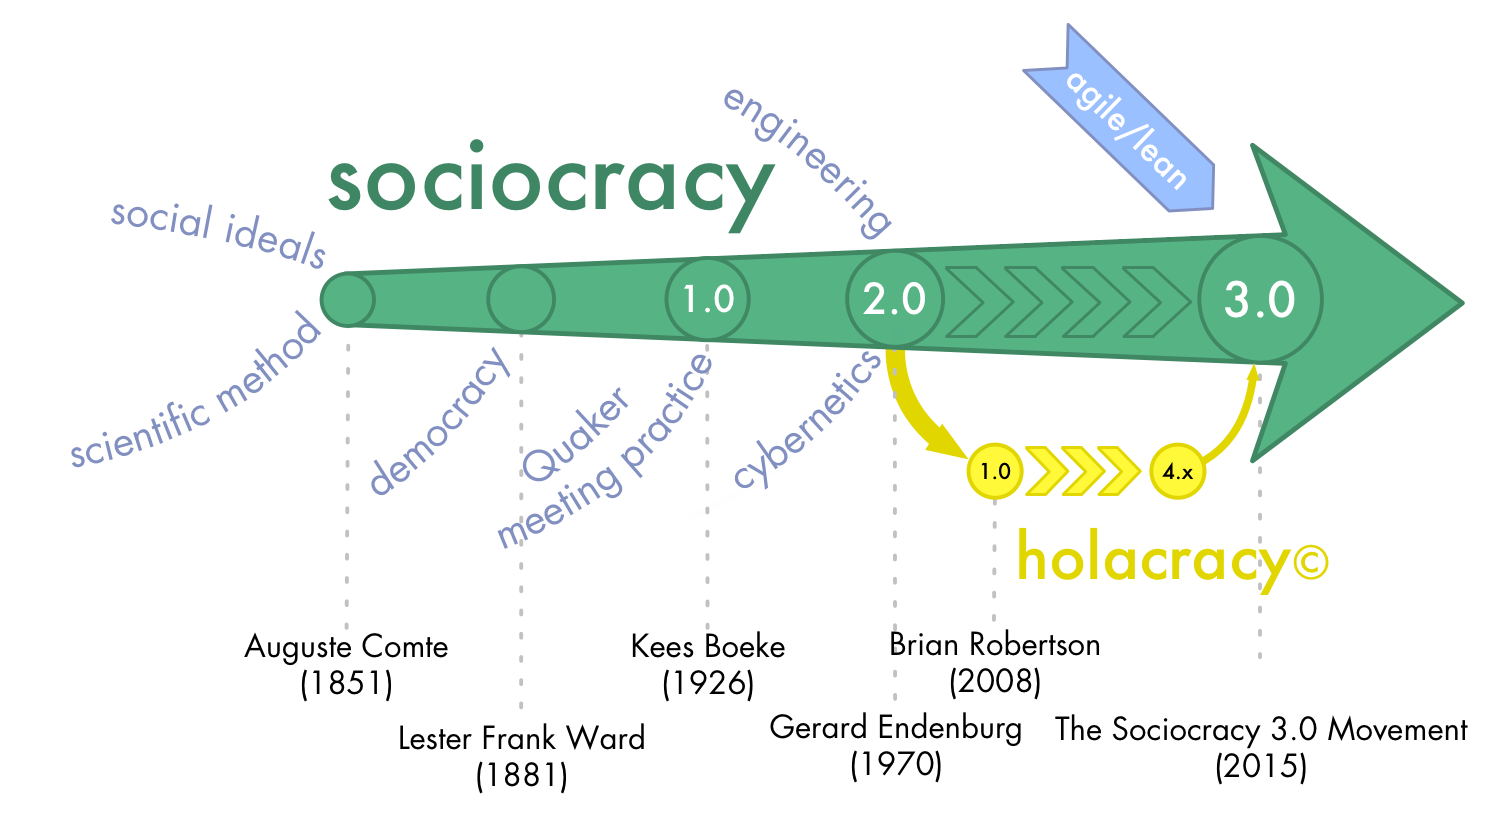
\includegraphics[keepaspectratio,width=\textwidth,height=0.75\textheight]{img/general/history.png}
\end{figure}

\begin{itemize}
\item 1851 – Auguste Comte

\begin{itemize}
\item Scientific method applied to society

\item Sociocracy is “\emph{the social order of the future}” - not yet achievable but inevitable!

\end{itemize}

\item 1881 – Lester Frank Ward

\begin{itemize}
\item redefined the term Sociocracy to describe the rule of the people with relationships with each other

\end{itemize}

\item 1926 --1954 - Kees Boeke

\begin{itemize}
\item Established the first sociocracy in his residential school (based on Quaker consensus principles)

\item Book “\emph{Sociocracy: Democracy as it might be}” (1945)

\end{itemize}

\item 1970's - Gerard Endenburg

\begin{itemize}
\item Student in Kees Boeke’s school

\item Integrated principles from Engineering and Cybernetics

\item In his company Endenburg Electrotechniek he evolved “\emph{The Sociocratic Circle-Organization Method}” (later becoming ``\emph{The Sociocratic Method}'')

\end{itemize}

\item 1978 - Sociocratisch Centrum Utrecht

\begin{itemize}
\item created to promote ``\emph{The Sociocratic Method}''

\end{itemize}

\item 1994 - New law in the Netherlands

\begin{itemize}
\item Sociocratic organizations are no longer required to have a worker’s council

\end{itemize}

\item 2000 - emergence of a now wide-spread grassroots movement

\item 2007 - \emph{We the People}

\begin{itemize}
\item John Buck \slash  Sharon Villines make Sociocracy accessible to the English-speaking world

\end{itemize}

\item 2014 The Sociocracy 3.0 Movement is born

\end{itemize}

\chapter{The S3 Movement}
\label{thes3movement}

The S3 Movement is a \textbf{distributed network consultants and trainers} from a variety of fields, who{\ldots}

\begin{itemize}
\item {\ldots}dedicate their time to developing and evolving S3 to make it \textbf{available and applicable to as many organizations as possible}.

\item {\ldots}provide resources under a \textbf{Creative Commons Free Culture License} to learn, practice and teach Sociocracy 3.0.

\item {\ldots}share a deep appreciation for the transformational potential of S3 to help organizations and their members thrive.

\end{itemize}

\chapter{Why ``Sociocracy 3.0''}
\label{whysociocracy3.0}

\textbf{Respect to the lineage of Sociocracy, and a step forward:}

\begin{itemize}
\item an approach towards organizational change that meets organizations where they are

\item integrated with lean and agile thinking

\item new ways to evolve organizational structure

\item patterns for all aspects of collaboration, not just for governance

\end{itemize}

\section{Design Goals}
\label{designgoals}

\begin{figure}[htbp]
\centering
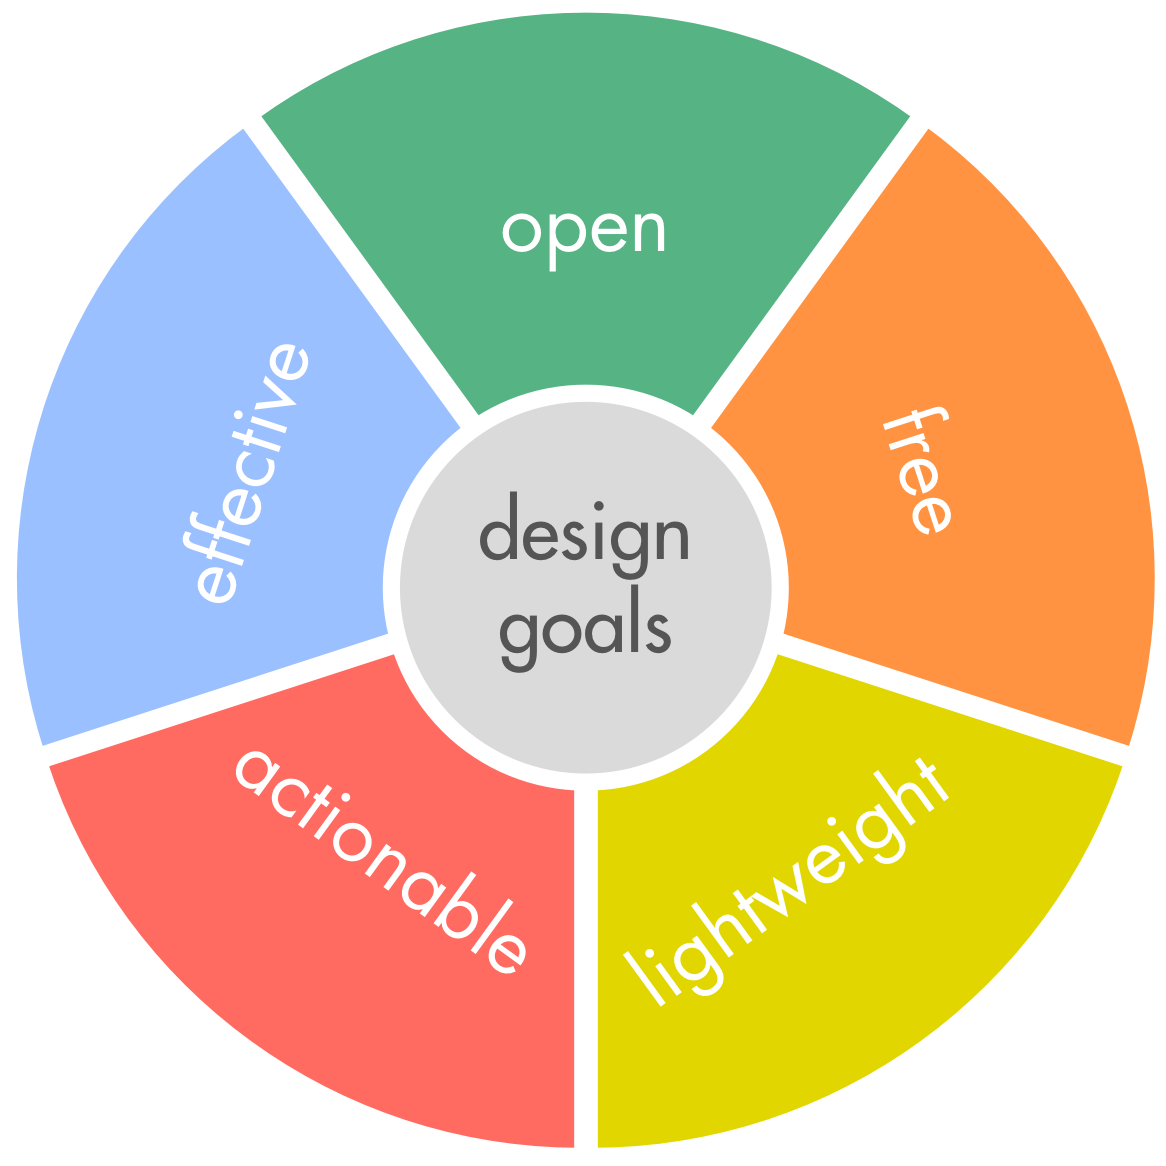
\includegraphics[keepaspectratio,width=\textwidth,height=0.75\textheight]{img/general/design-goals.png}
\end{figure}

\textbf{Open}: Principle-based and modular patterns make it easy to choose and adapt according to context

\begin{itemize}
\item do with it what you want

\item take just what you need

\item remix, extend and adapt it as you like

\end{itemize}

\textbf{Free}: Un-centralized distribution and a Commons license eliminates barriers to entry:

\begin{itemize}
\item free and accessible resources

\item no hidden fees

\item no certifications

\item no small print

\end{itemize}

\textbf{Effective}: Principles and patterns have been tried and tested in many organizations, often for decades.

\begin{itemize}
\item need-driven

\item value-driven

\item customer\slash user focus

\end{itemize}

\textbf{Actionable}: There's something any organization can use right now, regardless of their unique context. S3 contains lots of ideas anyone can try out within their area of influence.

\begin{itemize}
\item patterns for individuals

\item patterns for groups

\item patterns for organizations

\end{itemize}

\textbf{Lightweight}: Just the essentials: common-sense practices, bare-bone processes:

\begin{itemize}
\item free of stuff that gets in the way

\item no busywork or unnecessary bureaucracy

\end{itemize}

\{\{seven-principles.md\}\}

\chapter{Patterns}
\label{patterns}

A \textbf{pattern} is a template for successfully navigating a specific context.

S3 patterns are discovered through observing many organizations as they solve problems, innovate, and respond to opportunities. Patterns may need to be adapted and evolved to suit differing contexts and needs.

The more than 60 patterns on S3 are organized in 7 pattern groups.

\begin{figure}[htbp]
\centering
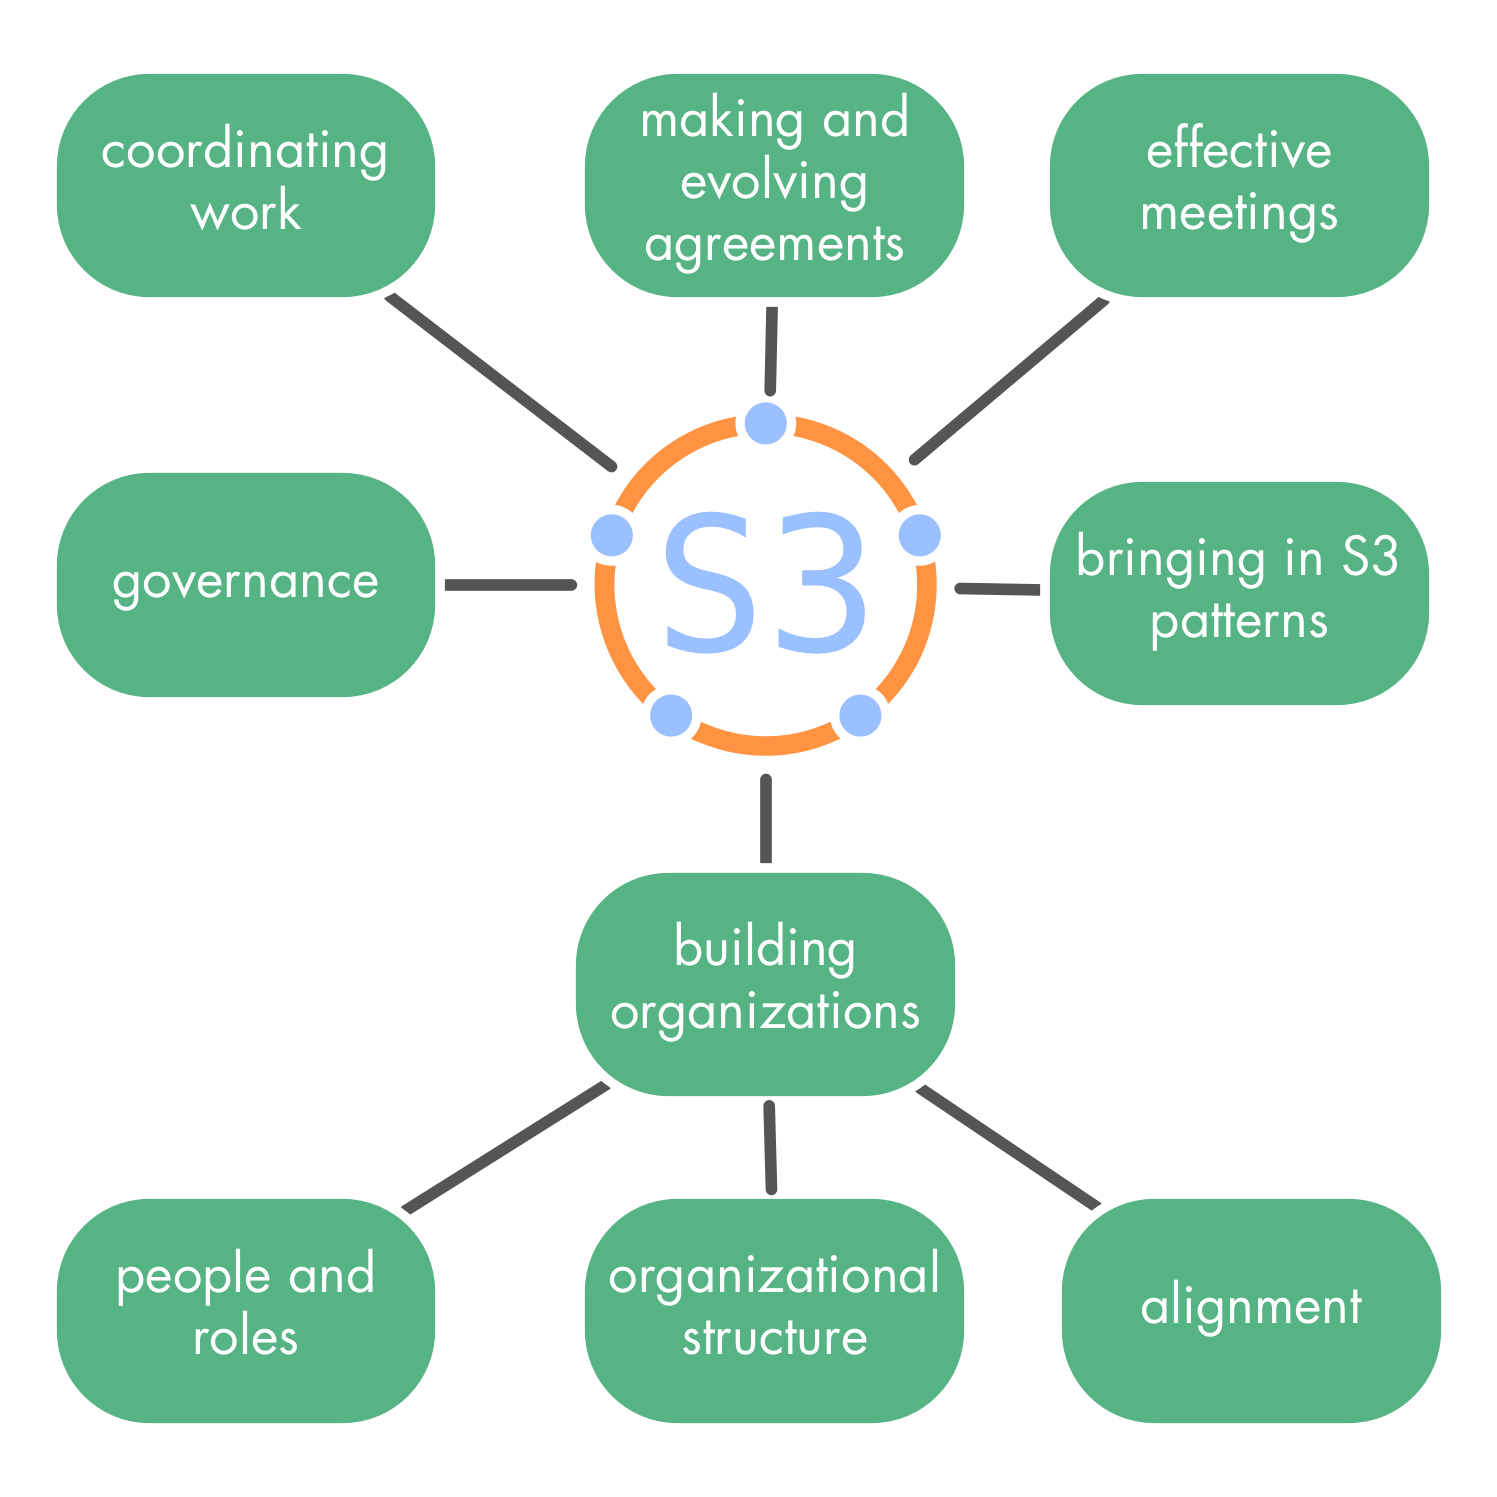
\includegraphics[keepaspectratio,width=\textwidth,height=0.75\textheight]{img/general/s3-pattern-groups.png}
\end{figure}

\part{The Patterns}
\label{thepatterns}

\chapter{Making And Evolving Agreements}
\label{makingandevolvingagreements}

The way we make, keep and evolve agreements largely determine both the effectiveness of collaboration and the happiness of an organization's members.

S3 contains patterns to cover you from identifying the motive for your actions and agreements (Driver), to co-creation of and commitment to an agreement (Proposal Forming and Consent Decision Making), to evaluating and evolving agreements (e.g. Evaluation Criteria, Intended Outcome, Deliverables).

{\ldots}

\section{Agreements}
\label{agreements}

We respond to drivers through agreements.

\textbf{Definition:} \emph{A agreement is an agreed upon guideline, pattern, process or protocol designed to guide the flow of value.}

\begin{itemize}
\item agreements are created in order to satisfy drivers

\item agreements are the \textbf{accountability of the circle} that created them

\item each agreement includes \textbf{evaluation criteria} and is subject to \textbf{regular review}

\begin{itemize}
\item review dates are specific to each agreement

\item agreements are reviewed in context to its driver

\end{itemize}

\end{itemize}

\begin{figure}[htbp]
\centering
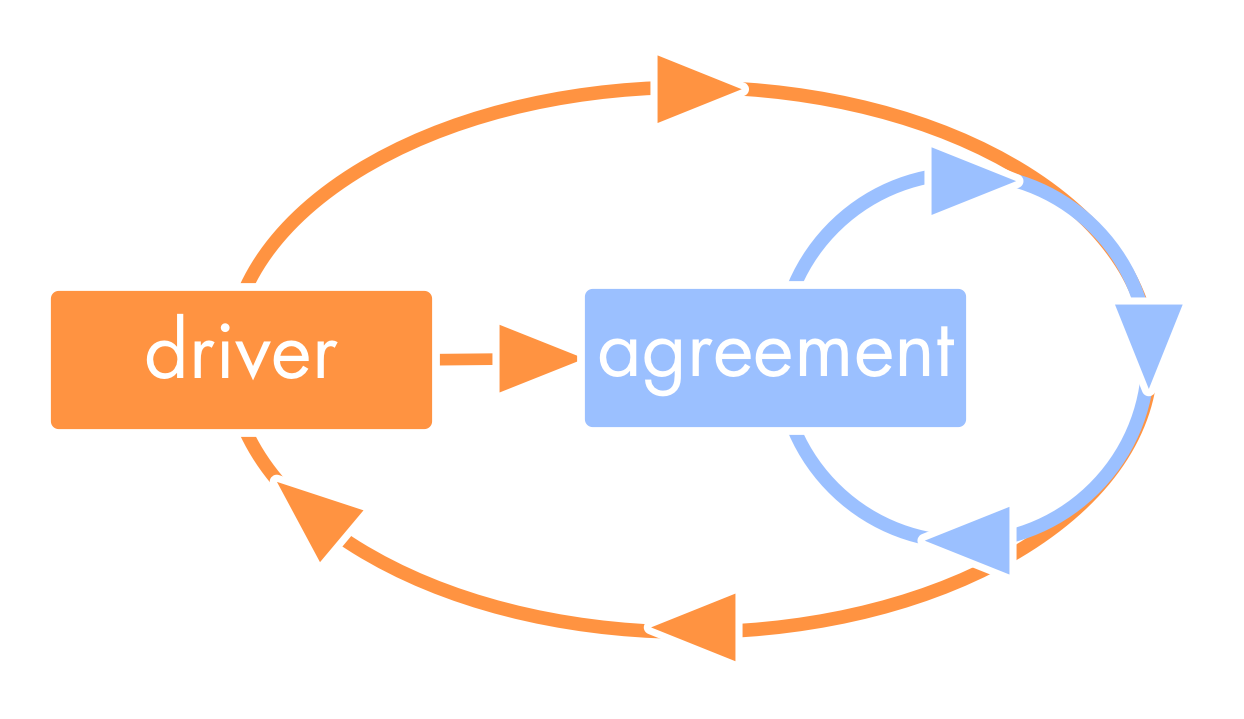
\includegraphics[keepaspectratio,width=\textwidth,height=0.75\textheight]{img/tension-driver-domain/driver-agreement-improvement.png}
\end{figure}

\subsection{Template for Agreements}
\label{templateforagreements}

\begin{figure}[htbp]
\centering
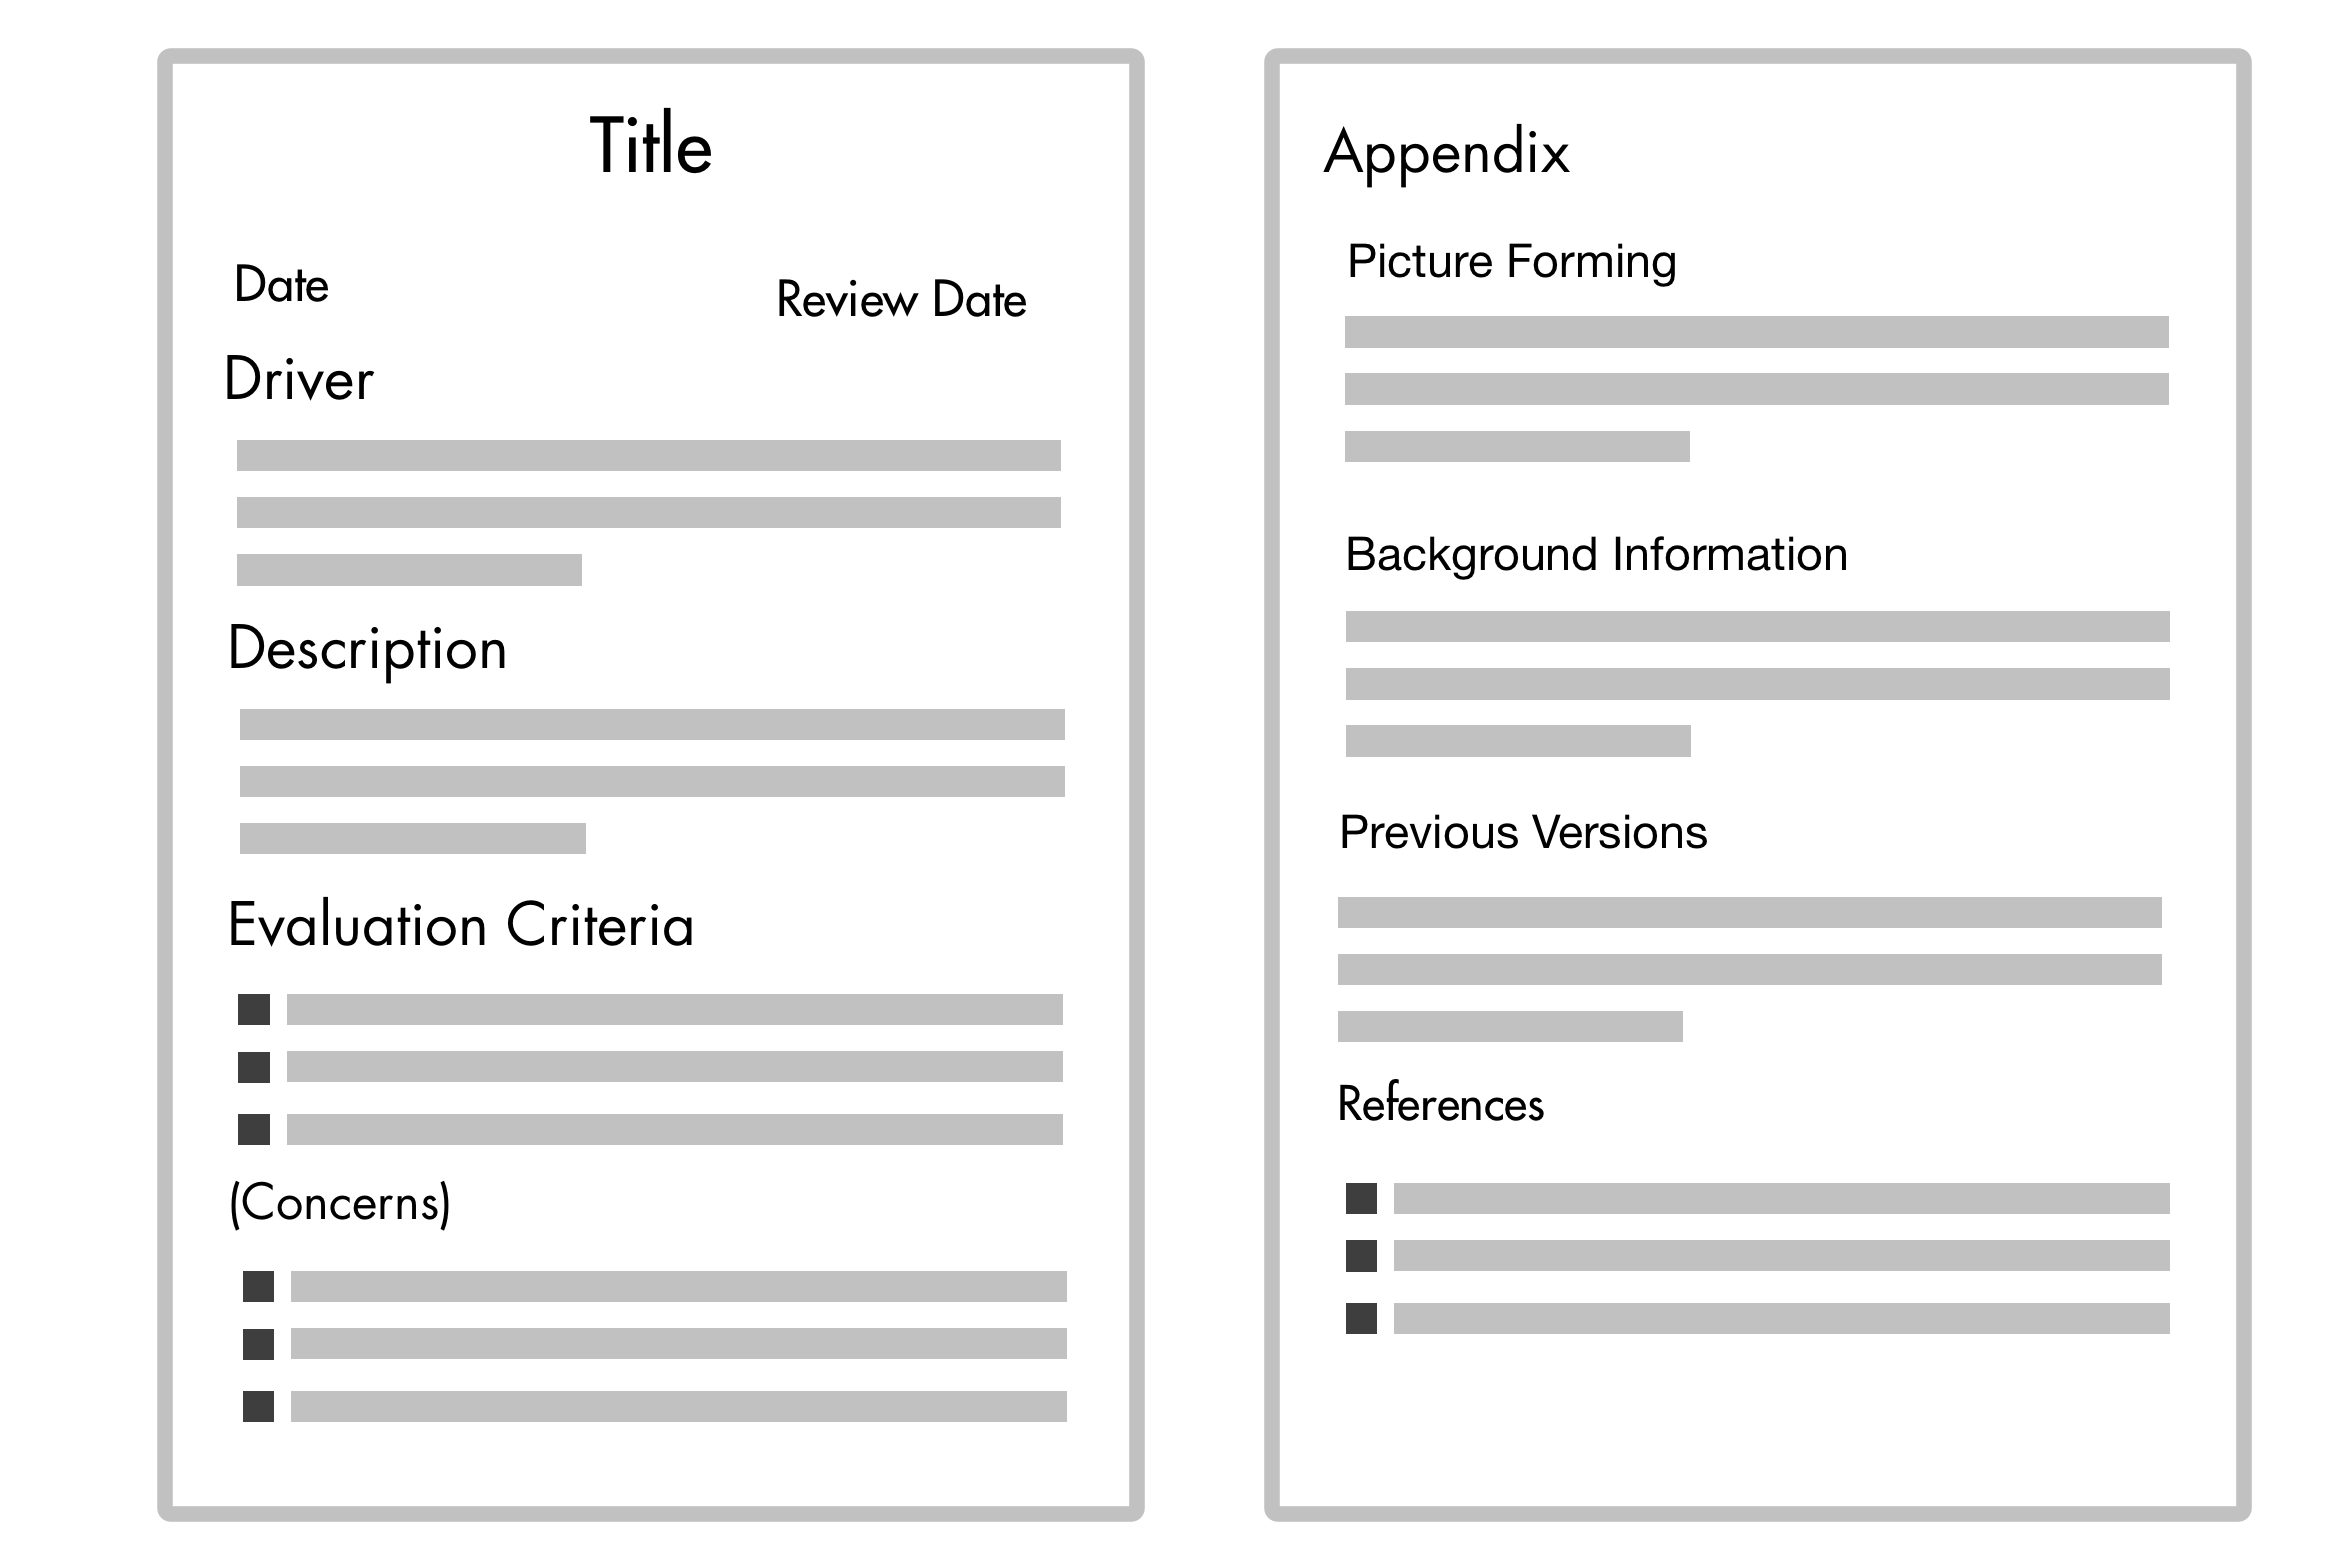
\includegraphics[keepaspectratio,width=\textwidth,height=0.75\textheight]{img/agreements/agreement-template.png}
\end{figure}

\section{Circle}
\label{circle}

A circle{\ldots}

\begin{itemize}
\item {\ldots}is the basic building block of an organization

\item {\ldots}is a group of people gathered around a driver (permanent or temporary)

\item {\ldots}makes all agreements by consent

\item {\ldots}is accountable for its own development

\end{itemize}

\textbf{Definition:} \emph{A circle is a semi-autonomous, self-organizing and self-governing group of people gathering around a driver.}

\begin{figure}[htbp]
\centering
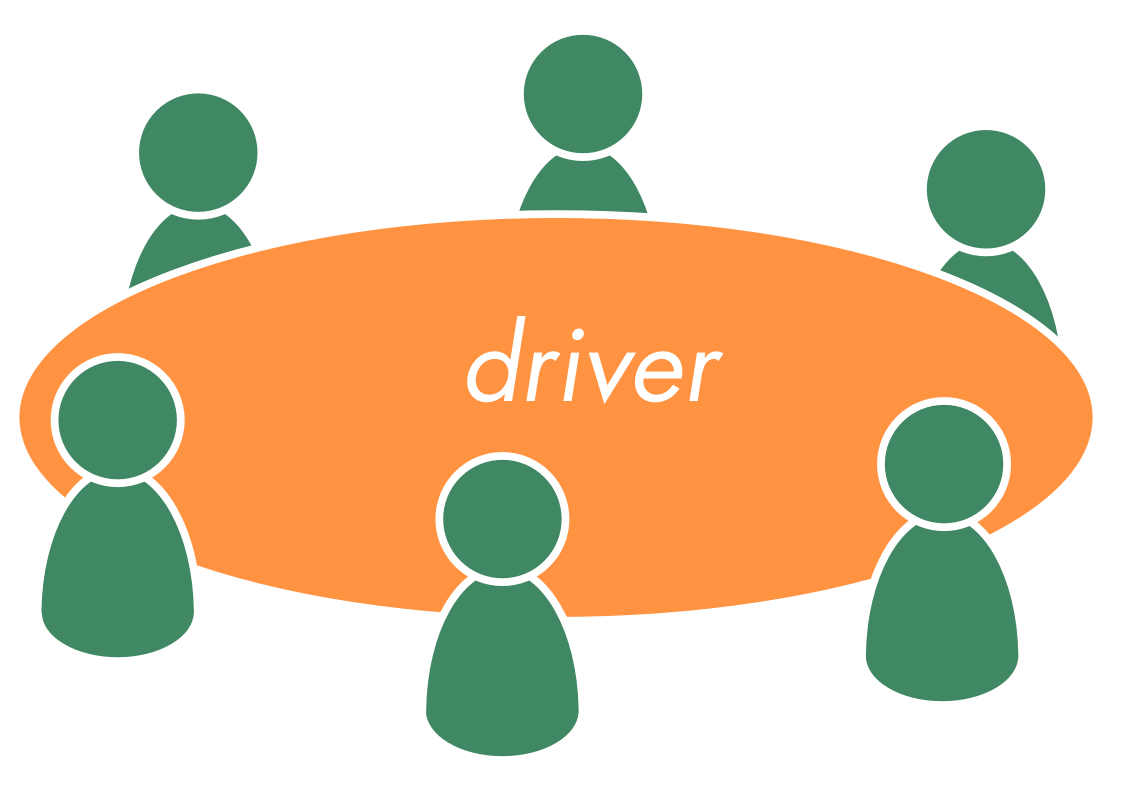
\includegraphics[keepaspectratio,width=\textwidth,height=0.75\textheight]{img/circle/circle-driver.png}
\end{figure}

\begin{itemize}
\item {\ldots}\textbf{semi-autonomous}:

\begin{itemize}
\item each has a unique driver and can create value independently

\end{itemize}

\item {\ldots}\textbf{self-organizing}:

\begin{itemize}
\item independent in organizing day-to-day-work

\end{itemize}

\item {\ldots}\textbf{self-governing}:

\begin{itemize}
\item independent in creating strategy and agreements

\end{itemize}

\end{itemize}

\section{Consent Decision Making}
\label{consentdecisionmaking}

\begin{itemize}
\item Consent is the absence of objections

\begin{itemize}
\item everyone affected by a decision can ``live with it''

\item consent is not consensus with unanimity

\end{itemize}

\item Consent is used to make and evolve all agreements in a circle

\item Objections stop proposals becoming agreements

\item Withholding objections could harm the aims of a group or organization

\item Being able to raise objections at any time means that proposals only need to be \emph{good enough for now, safe enough to try}

\item Every agreement has a review date

\end{itemize}

Consent Decision Making{\ldots}

\begin{itemize}
\item is a facilitated decision making process

\item deliberately harvests reasoned objections in order to integrate the wisdom they contain in proposals or existing agreements

\item helps balance equivalence and effectiveness

\item experienced groups can move quickly through the stages of Consent Decision Making

\end{itemize}

\subsection{Harvesting Objections to Capture Emergent Wisdom}
\label{harvestingobjectionstocaptureemergentwisdom}

\begin{figure}[htbp]
\centering
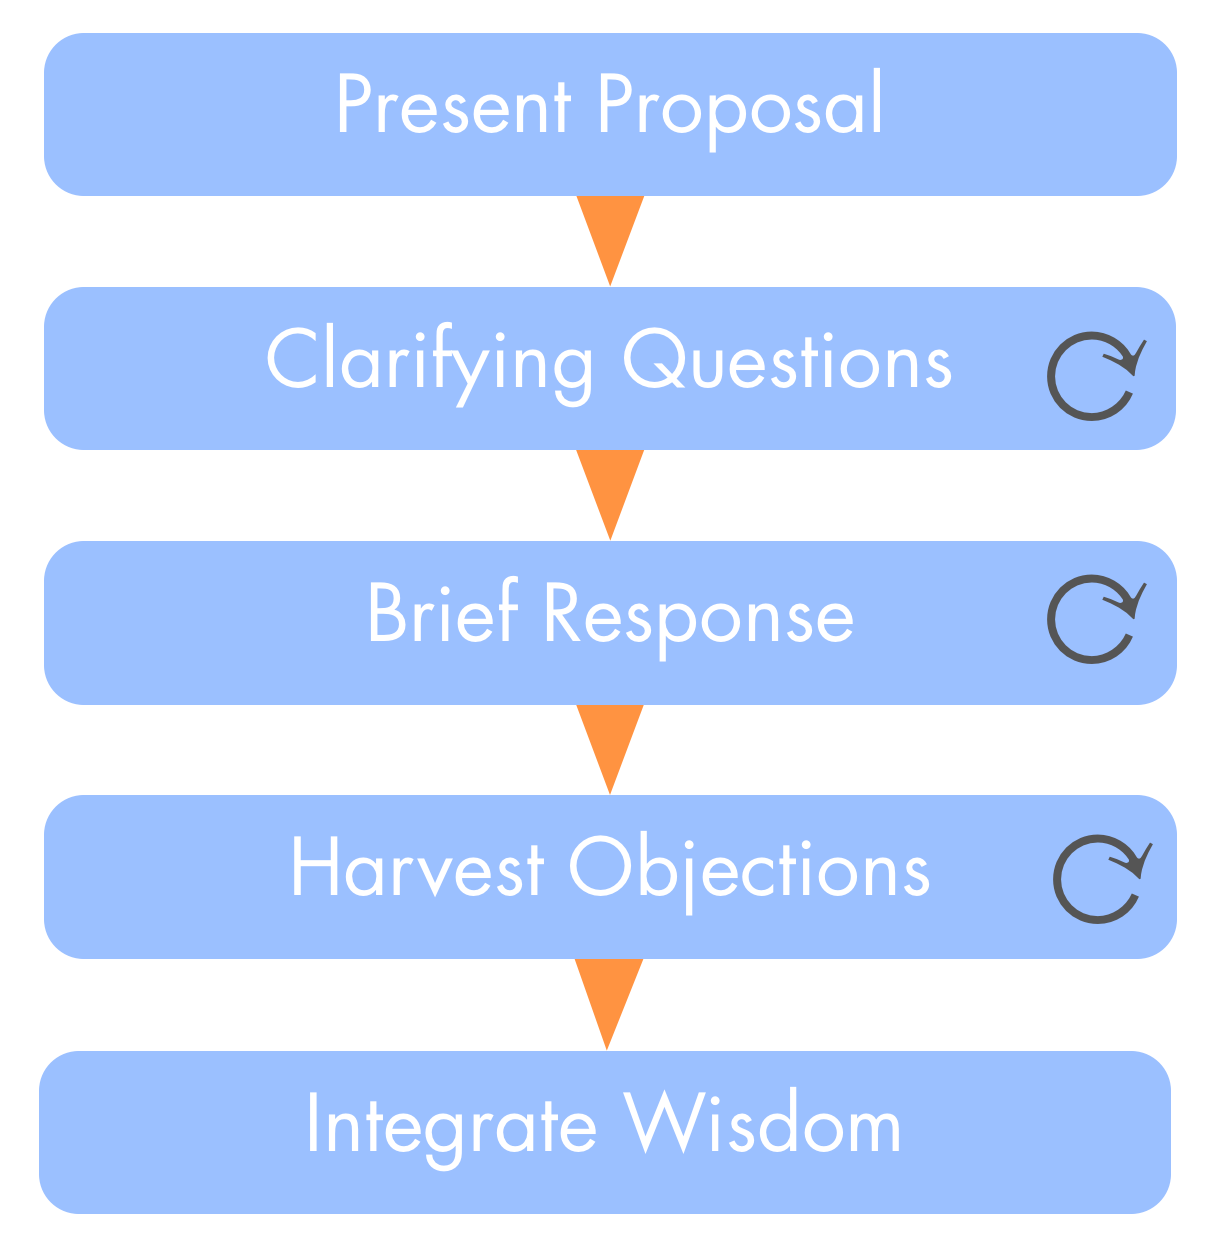
\includegraphics[keepaspectratio,width=\textwidth,height=0.75\textheight]{img/agreements/cdm-condensed.png}
\end{figure}

\section{Deliverables}
\label{deliverables}

A \textbf{deliverable} is something which is provided as a result of an agreement, usually framed as a product or a service. Deliverables can be defined for organizational strategy, circle strategy, \emph{development plans}, \emph{role descriptions}, or any other \emph{agreement}.

Since a deliverable is part of an agreement, make sure the amount of detail is reasonable - sufficient to allow for shared understanding, but not too much. Consider the context in which and by whom this description will be referred to. Think about the significance of the deliverable, and how long this description needs to be referred to.

For example simple task which will be implemented in the next week needs less written detail than continuously reviewing updates for a large product for compliance with several complicated national standards.

Reference other documents when helpful or necessary, e.g. contracts, previous projects, specifications, drafts, or other agreements.

\section{Driver}
\label{driver}

The \textbf{driver} is the reason and the motivation for action in a specific situation: the needs a team or organization identifies and chooses to address, and the conditions relevant to understanding these needs.

\{$>$$>$ older version: A \textbf{driver} is what motivates us into action in a specific situation: the \textbf{needs} we perceive, and the \textbf{conditions} from which these needs arise. $<$$<$\}

A driver can apply to an individual, or describe \textbf{collective motivation for a group}. Developing shared understanding of drivers fosters \textbf{alignment towards the motive} instead of towards our assumptions about the future. The response to a driver always involves the \textbf{adaptation of an existing agreement, or creation of a new one}, including:

\begin{itemize}
\item changing the plan: adding a task or project

\item adaptation or creation of a role

\item creation of a new circle

\end{itemize}

However, sometimes we may decide against responding to a driver, because there is more important things to tend to.

\subsubsection{Needs and Conditions}
\label{needsandconditions}

A \textbf{need} is the lack of something that is necessary (required?) or important

Needs are identified when analyzing a situations, and may related to the organization itself, its members, stakeholders, customers or the environment.
Needs can be objective (physical) or subjective (psychological), and may be controversial on a social level. An organization's values may help resolving controversies

Some examples for needs, from more abstract needs to personal needs:

\begin{itemize}
\item revenue, profit, shareholder value, capital

\item customer value

\item autonomy, mastery, purpose

\item connection, collaboration, recognition

\item sustenance, happiness

\end{itemize}

Each need emerges through one or several conditions. In order to understand a driver, we need to identify relevant and important conditions for each need, and describe them, usually as facts or observations.

Over time, we will develop better understanding of a driver, and, as the needs and conditions change, update the driver's description.

We review a review whenever we review a strategies or agreements which respond to that driver. In a driver review we discover new or changed needs and conditions, sometimes the driver no longer falls into our domain, or is no longer relevant.

\subsection{Drivers and Lean Thinking}
\label{driversandleanthinking}

\subsubsection{Value and Waste}
\label{valueandwaste}

Lean Thinking is centered around the ideas of value and waste, both can easily be defined in relation to a driver:

\begin{itemize}
\item \textbf{value} is the importance, worth or usefulness of something for responding to a driver.

\item \textbf{waste} is anything not necessary (or essential) for - or standing in the way of - effective response to a driver.

\end{itemize}

In this context, value is \textbf{not} an \textbf{inherent} property as it only exists in relation to a driver. This is why value is not necessarily expressed in currency or time, but it often can be quantified by identifying metrics related to the needs or conditions contained in a driver.

Adopting the concept of value and waste makes many tools and ideas from \textbf{lean production} and \textbf{lean software development} available to support organizations running on Sociocracy 3.0:

\begin{itemize}
\item value stream mapping

\item various strategies for eliminating waste

\item the Kanban Method

\end{itemize}

\subsubsection{Waste and Continuous Improvement}
\label{wasteandcontinuousimprovement}

\begin{figure}[htbp]
\centering
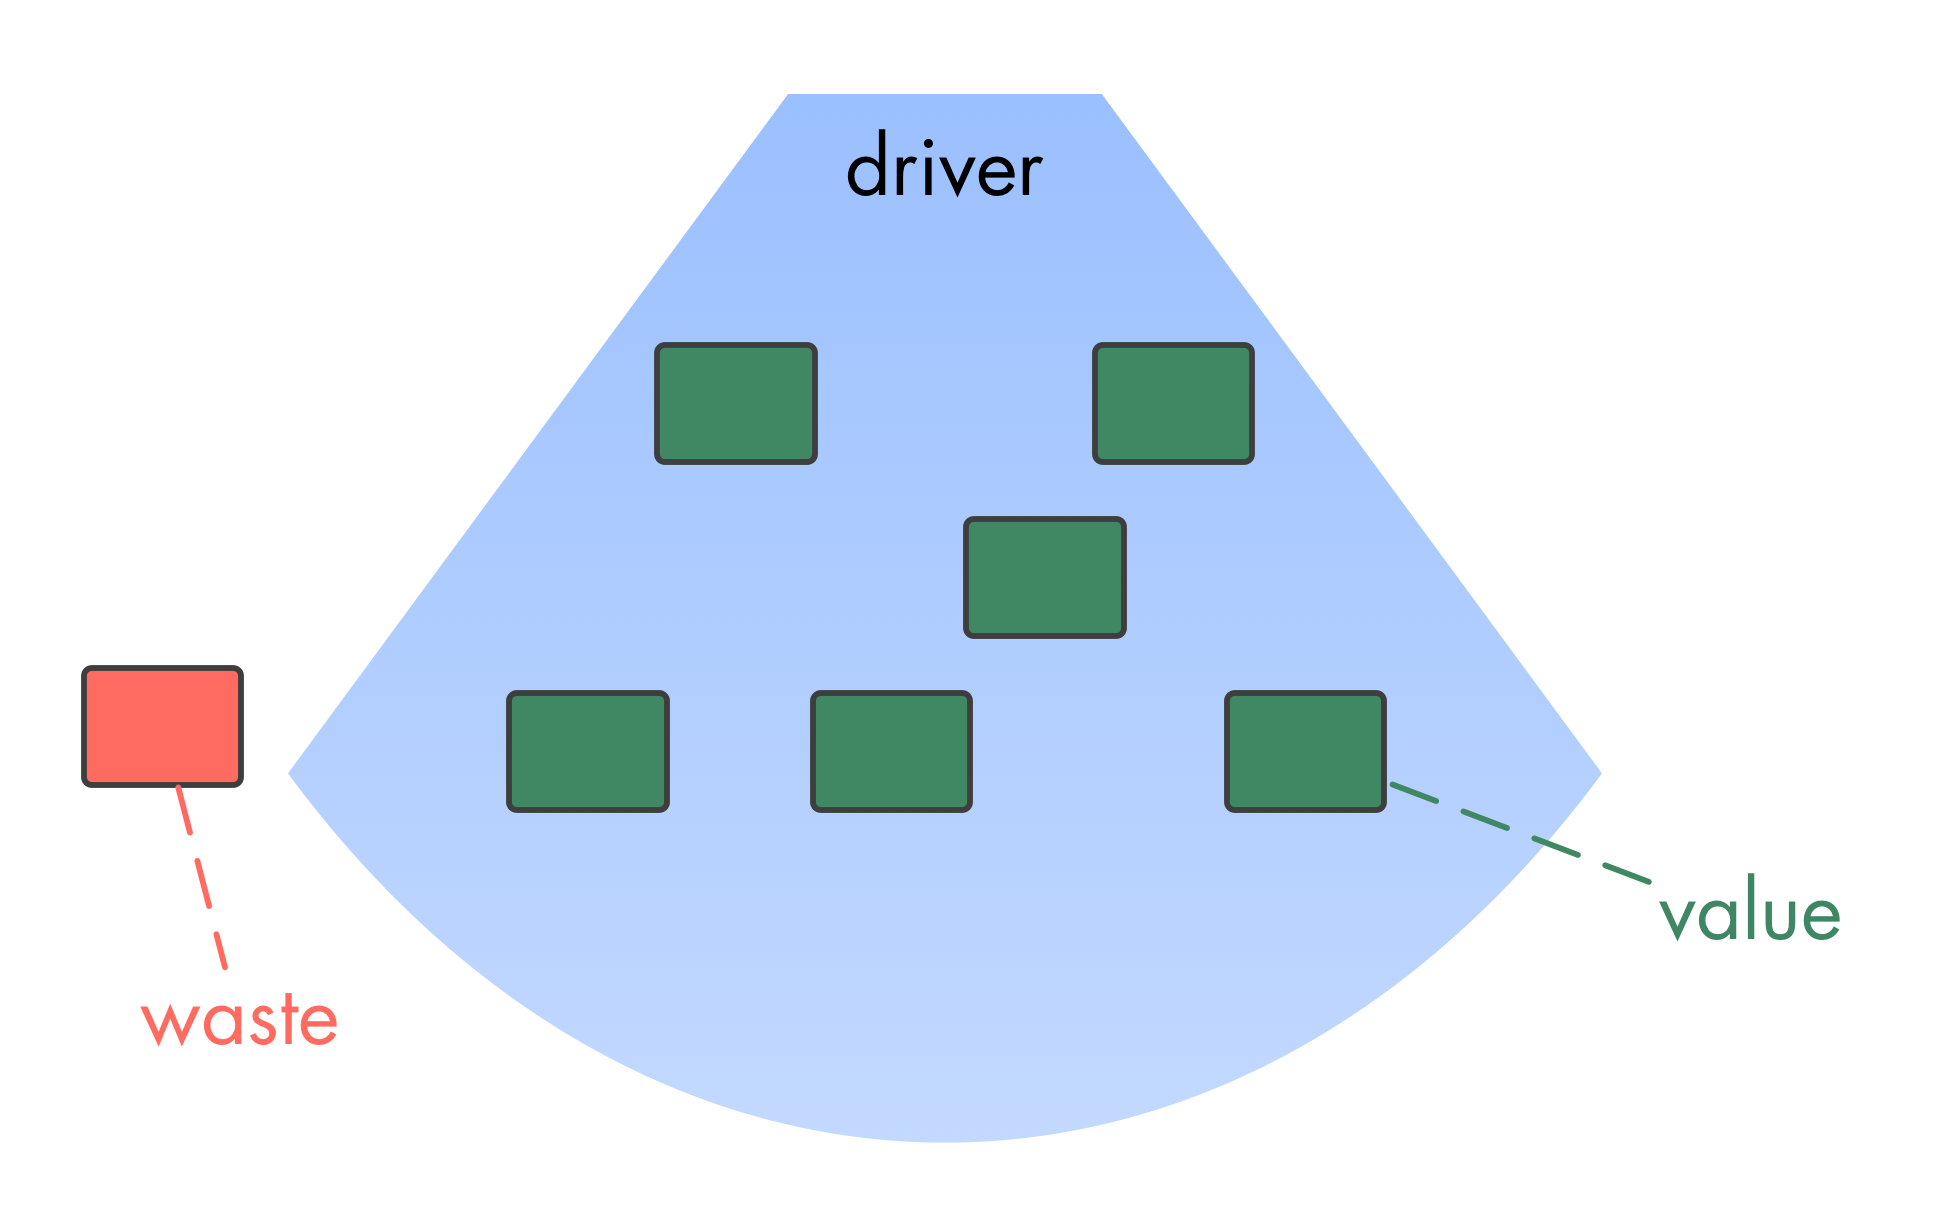
\includegraphics[keepaspectratio,width=\textwidth,height=0.75\textheight]{img/workflow-and-value/drivers-value-waste.png}
\caption{Identifying Waste}
\end{figure}

Waste exist in many different forms and on different levels of abstraction, e.g. in tasks, agreements, work processes, organizational structure or mental models. Waste makes itself known as tensions, learning learning to identify waste is a long journey, but along the way we also discover wisdom that helps us evolve our understanding of our drivers.

Establishing a process for ongoing elimination of waste enables the natural evolution of an organization towards greater effectiveness, optimizing the flow of value through an organization. As a side effect, the organization will so naturally adapt to changes in the environment.

\section{Evaluate Agreements}
\label{evaluateagreements}

A pattern for ensuring agreements remain effective.

\textbf{Motivation for this pattern:} To keep an organization's or team's body of agreements effective in the face of emerging knowledge and changes in context, each agreement needs to be periodically reviewed and updated.

\textbf{Agreements}\footnote{in some organizations these agreements are referred to as a ``policy'').} guide action and behavior. They are created as a response to a specific situation that affects an organization or team.

Team and organization wide agreements are kept up-to-date with what is happening, what is learned, and how expectations compare to actual outcomes.

\subsection{Indicators for this pattern}
\label{indicatorsforthispattern}

\textbf{Conditions:}

\begin{itemize}
\item existing agreements don't make sense any more (out of date, slow, rigid, ineffective)

\item lack of clarity about why things are done in certain ways and what outcomes an agreement is meant to have

\item lack of opportunities taken to integrate new learning and improve

\end{itemize}

\textbf{Needs:}

\begin{itemize}
\item adapting to changes in the inner and outer environment of the organization

\item improve and evolve agreements previously made

\item integrate learning from new experiences

\end{itemize}

\subsection{The Details}
\label{thedetails}

Changes in context can make an agreement less effective or even obsolete. Putting an agreement into action often reveals new ways an agreement can be improved.

Organizations or teams periodically evaluate their agreements, usually in periodical meetings, or even a dedicated workshop to review a complex agreement (e.g. an organization's values or strategy).

Evaluating agreements has \textbf{four basic steps}:

\begin{enumerate}
\item preparation

\item hear reports (optional)

\item the actual review

\item addressing any consequences

\end{enumerate}

\subsubsection{Step 1 - Preparation}
\label{step1-preparation}

Preparing for the review helps to keep it brief and effective.

Inform everyone affected of the upcoming review and make sure they have access to documents describing the agreement and its iterations, and if applicable, data relating to evaluation criteria and metrics.

Ensure all documents related to the agreement are up to date, and reports are prepared (see next step).

\subsubsection{Step 2 - Hear Reports}
\label{step2-hearreports}

For more complex agreements its useful to have a temporary ``owner'' who is familiar with the agreement and its effects. They review the evaluation criteria and other data and prepare a short report.

In some cases it may require several people to prepare and present a report.

The report is presented immediately before the actual review.

\subsubsection{Step 3 - The Review}
\label{step3-thereview}

The review itself is often split in two parts:

\begin{itemize}
\item review of the motive for the agreement

\item review of the agreement itself

\end{itemize}

\paragraph{Review the motive}
\label{reviewthemotive}

In order to prime the group about the context, it's a good idea to first review the motive for creating the agreement, i.e. needs or requirements the agreement should address, and the conditions or context in which the needs or requirements were identified.

If an agreement does not contain a description of the motive, this may be a good time to collaborate on describing it.

Helpful questions to review the motive include:

\begin{itemize}
\item \emph{Is the description of the motive still accurate, or does it need to change?} (e.g. because we changed the conditions, learned something, or discovered something else is needed)

\item \emph{Is this situation still relevant for the organization or this team?}

\end{itemize}

\textbf{Sometimes the review ends here}, because:

\begin{itemize}
\item the authority to respond to the situation falls to someone else: Pass it to relevant team or individual

\item the motive for agreement no longer exists or ceased to be relevant: Close the agreement

\end{itemize}

In both cases, address any consequences (Step 4).

\paragraph{Review the agreement}
\label{reviewtheagreement}

Review the agreement itself in its latest form by asking these questions:

\emph{Considering any reports heard, the updated understanding of conditions and needs and what is known today:}

\begin{itemize}
\item \emph{Is the agreement still good enough for now and safe enough to try?}

\item \emph{Do you see any reason why NOT to continue with this agreement in its current form?}

\item \emph{Are there any concerns about this agreement?}

\end{itemize}

Depending on the answers to these questions there are several possible outcomes:

\begin{enumerate}
\item keep the agreement without change

\item use what's learned to update the agreement on the spot, or, for more substantial changes, schedule a separate session for the update

\item drop the agreement

\end{enumerate}

In all cases, consider recording answers and concerns for future evaluations, and \textbf{agree on a next review date.}

\subsubsection{Step 4 - Addressing any consequences}
\label{step4-addressinganyconsequences}

After the review, ensure consequences of any decisions are dealt with.

This may include:

\begin{itemize}
\item assigning tasks

\item recording the latest version of the agreement

\item updating other agreements affected by decisions made

\item sharing results with those affected by the decision

\item scheduling further pending decisions if required

\end{itemize}

\subsubsection{Considerations for an effective review process}
\label{considerationsforaneffectivereviewprocess}

Use the idea of \textbf{falsification} instead of merely focusing on what would make an agreement a success. Describe what would need to happen to consider that it failed. This information can be used to describe the intended outcome, and to define criteria for evaluation.

Adjust the review cadence according to the stability of the agreement.

Consider having an early review when people affected by the agreement raise concerns or explain reasons why continuing without change may not be effective, or how changing the agreement could improve effectiveness.

\subsection{Related patterns}
\label{relatedpatterns}

Agreements are evaluated in \emph{Governance Meetings} by the \emph{Circle} that created them.

The description of an agreement can include the \emph{Driver} it responds to, the \emph{Agreement} itself, any \emph{Intended Outcomes} and \emph{Evaluation Criteria}.

In Step 2 people review the \emph{Driver} of an agreement.

In Step 4 \emph{Consent Decision Making} can be used to test the agreement.

If the circle decides a new agreement is needed, its members might use \emph{Proposal Forming} to come up with one.

\section{Evaluation Criteria}
\label{evaluationcriteria}

Evaluation criteria help you understand whether or not an agreement has the desired effect.

Make them simple and unambiguous so you avoid discussing opinions when reviewing your agreements: Go for ``the number of items sent back from the customer for re-work should have dropped from 10 per week to 5 or less by January 10th'' instead of ``Quality is improved..''

One very effective way of defining Evaluation Criteria is as \emph{actionable metrics}, i.e. a set of measurements which you can continuously refer to to see whether you're on the right track. Actionable metrics make it easy to spot deviations from your intended outcome, and to take action accordingly. Consider this example: you have a steady trickle of new users for your website, and you want to increase popularity of your site. If you track number of website users per day, the graph will rise even without your new agreements being effective. However, tracking new users per day will give you a much clearer picture, if this metric is increasing, you know you're on the right track, and if it's shrinking, you know that you need to get together and take action.

\begin{figure}[htbp]
\centering
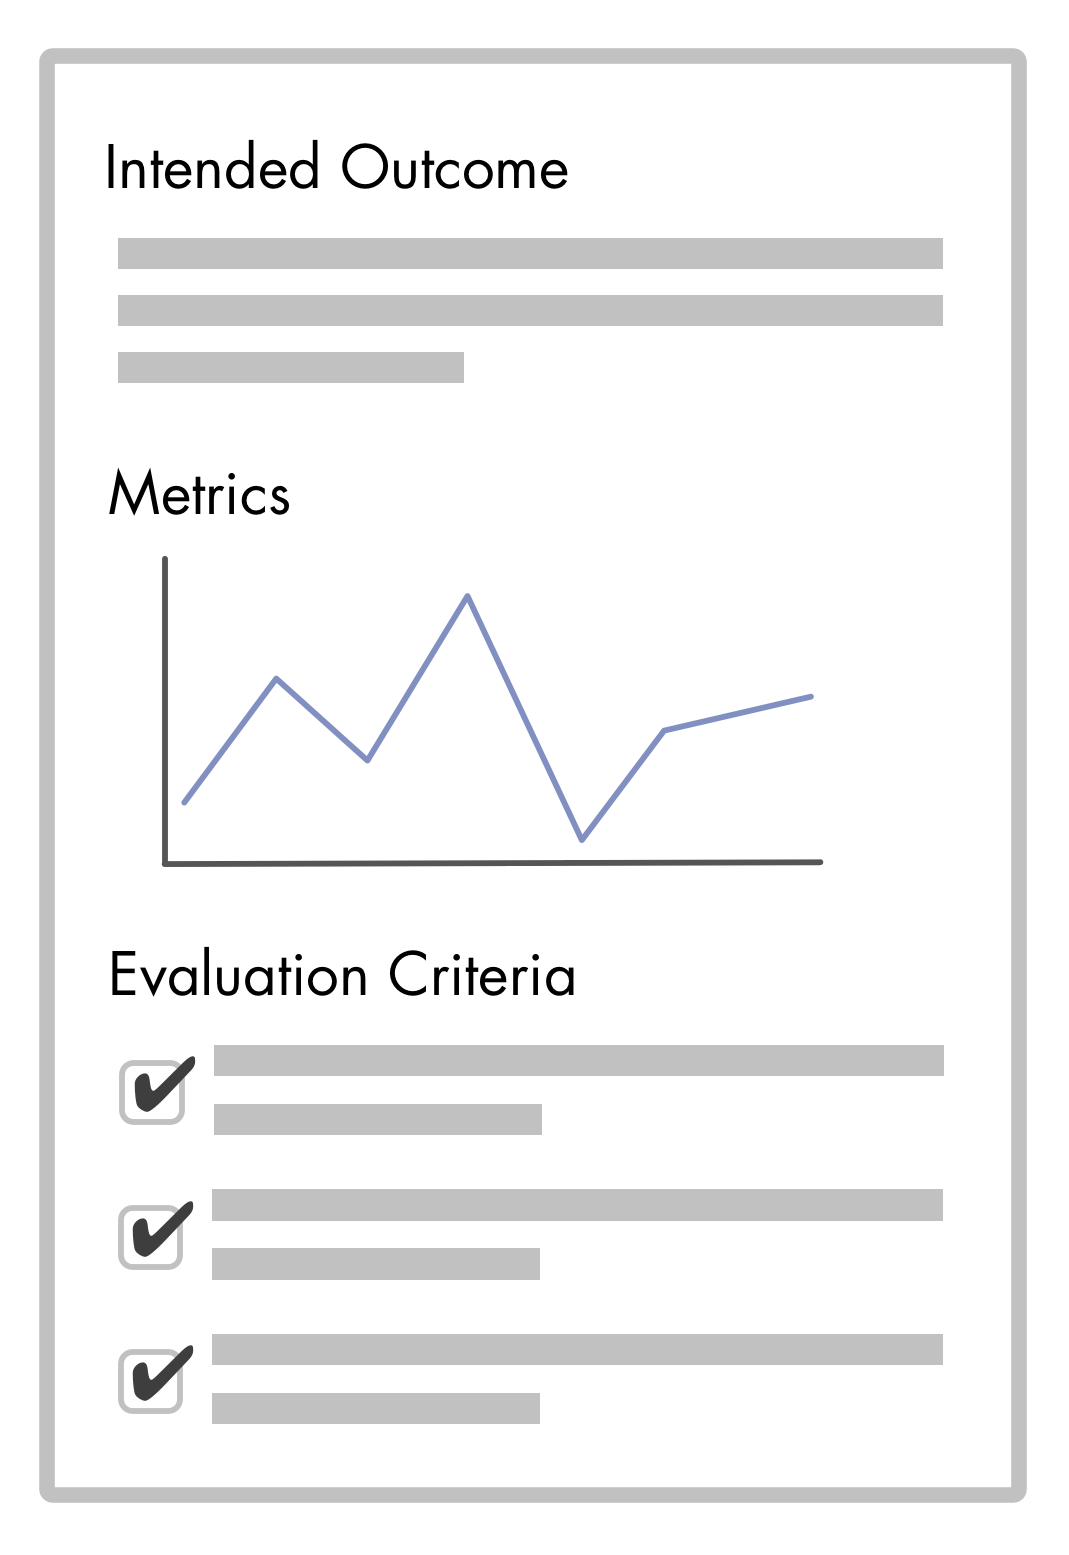
\includegraphics[keepaspectratio,width=\textwidth,height=0.75\textheight]{img/agreements/outcome-and-criteria.png}
\end{figure}

\section{Intended Outcome}
\label{intendedoutcome}

The \emph{Indended Outcome} is a brief description of what we expect to happen as the result of an agreement or strategy. It's a good idea to also include specific \emph{Evaluation Criteria} to enable an effective review of the strategy or agreement.

\begin{figure}[htbp]
\centering
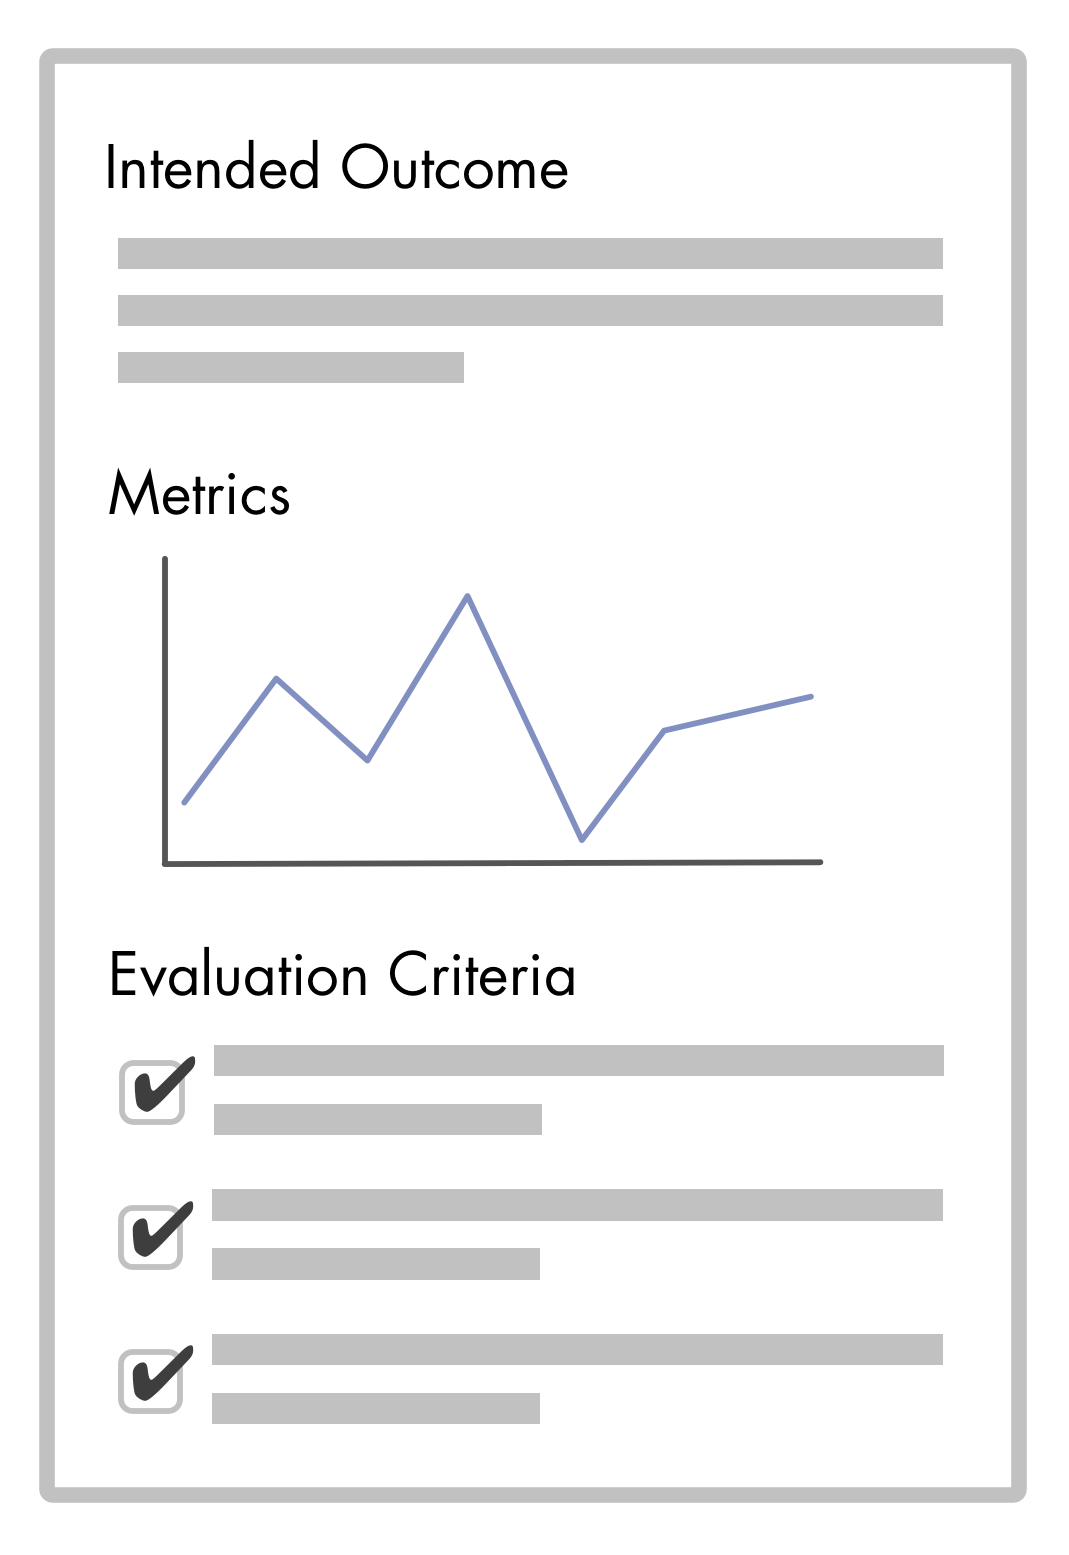
\includegraphics[keepaspectratio,width=\textwidth,height=0.75\textheight]{img/agreements/outcome-and-criteria.png}
\end{figure}

\section{Objections}
\label{objections}

\textbf{Definition:} \emph{An objection is a reason why doing what is proposed stands in the way of (more) effective satisfaction of an existing driver.}

In sociocracy we deliberately seek objections as they reveal
wisdom that can be used to improve proposals and agreements.

Objections{\ldots}

\begin{itemize}
\item {\ldots}are gifts

\item {\ldots}reveal wisdom seeking expression into the consciousness of a circle

\item {\ldots}reveal opportunities or impediments

\item {\ldots}emerge through individuals and belong to the whole circle

\item we love objections in sociocracy

\end{itemize}

\subsection{Questions That Help to Validate Objections}
\label{questionsthathelptovalidateobjections}

\begin{itemize}
\item Does the objection relate to this specific proposal or agreement?

\item Does this objection reveal how a (proposed or existing) \textbf{agreement}{\ldots}

\begin{itemize}
\item {\ldots}jeopardizes the satisfaction of a driver?

\item {\ldots}is in conflict with the organization's values?

\item {\ldots}prevents or diminishes someone's contribution to satisfying a driver?

\item {\ldots}can be improved significantly?

\end{itemize}

\end{itemize}

\section{Concerns{\ldots}}
\label{concerns...}

\begin{itemize}
\item {\ldots}are not objections

\item {\ldots}don't stop us from making agreements

\item {\ldots}often contain wisdom

\item {\ldots}can be recorded in the logbook

\begin{itemize}
\item {\ldots}to further evolve agreements

\item {\ldots}to set evaluation criteria (including review date)

\end{itemize}

\end{itemize}

\section{Proposal Forming}
\label{proposalforming}

Proposal Forming{\ldots}

\begin{itemize}
\item {\ldots}is similar to condensed design thinking process

\item {\ldots}taps the collective intelligence of a group

\item {\ldots}involves people in co-creating agreements

\item {\ldots}fosters accountability and a sense of ownership

\end{itemize}

\begin{figure}[htbp]
\centering
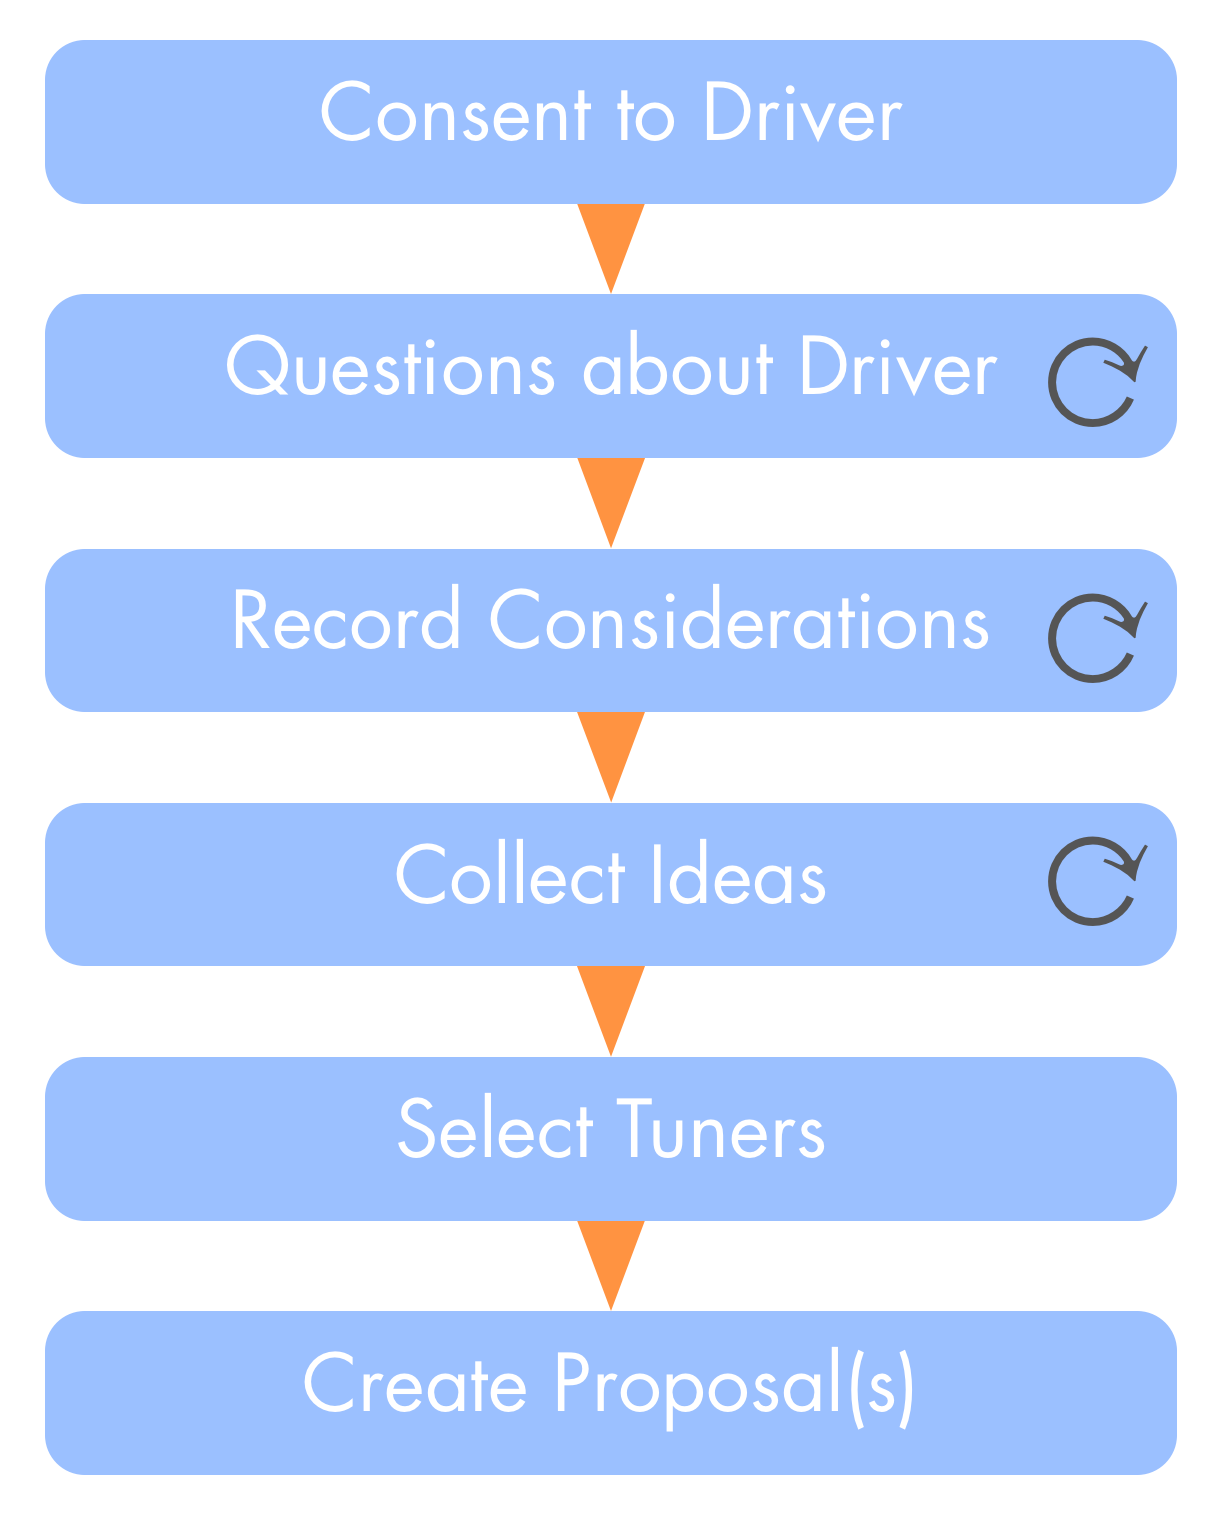
\includegraphics[keepaspectratio,width=\textwidth,height=0.75\textheight]{img/agreements/proposal-forming-medium.png}
\caption{Co-Creating a Response to a Drivers}
\end{figure}

\subsection{Proposal Forming Process}
\label{proposalformingprocess}

\begin{enumerate}
\item \textbf{Identify} the driver

\item \textbf{Consider}: Collect considerations as questions that reveal the scope of the issue

\item \textbf{Create}: Gather ingredients\slash ideas for solutions

\item \textbf{Refine}: Design a proposal from some or all of the ingredients

\item \textbf{Review}: process with consent decision making

\end{enumerate}

\section{Qualifying Drivers}
\label{qualifyingdrivers}

A pattern for{\ldots}

\textbf{Driver:}

Summary

\section{In a General Context}
\label{inageneralcontext}

\begin{itemize}
\item depending on our sensitivity, we might discover many different drivers

\item some of the drivers we identify are not in our domain

\item some drivers are more important than others

\item discussing every driver with the circle may be not effective

\item we need to make a conscious choice which drivers respond to, where to respond to them, and to discuss in the circle in the first place

\end{itemize}

We consider why, how and when to respond to a stimulus, instead of defaulting to action.

\begin{quote}

\emph{Between stimulus and response there is a space. In that space is our power to choose our response. In our response lies our growth and our freedom.} (Viktor E. Frankl)
\end{quote}

The individual sensing a tension is accountable for understanding the driver and making a decision on how to proceed, whether do drop it or refer the driver to a domain (a circle or a role). In that domain, we again make a decision whether or not to act on the driver.

\subsection{Individual Process}
\label{individualprocess}

\begin{itemize}
\item understand and describe driver

\begin{itemize}
\item what's happening and what's needed. relate each need to the conditions relevant for its existence

\end{itemize}

\item Can you identify the domain (circle or role) to address this driver?

\begin{itemize}
\item No: decide where to refer the driver to, or drop it.

\item Yes: refer driver to circle or role (e.g. add it to Governance Backlog)

\end{itemize}

\end{itemize}

\subsection{Circle or Role Process}
\label{circleorroleprocess}

\begin{itemize}
\item understand the driver

\begin{itemize}
\item refine and consent to driver description

\item Would responding to driver improve flow of value in this domain?

\begin{itemize}
\item Yes: Is it important to act on this now?

\begin{itemize}
\item Yes: decide what to do, and do it.

\item No: Drop it, put it in backlog, or schedule it for review?

\end{itemize}

\item No: Might responding to driver improve flow of value in another domain?

\begin{itemize}
\item Yes: refer driver to that domain

\item No: Drop it

\end{itemize}

\end{itemize}

\end{itemize}

\end{itemize}

\section{Resolve Objections}
\label{resolveobjections}

\textbf{Driver}:

\begin{itemize}
\item making decisions by consent invites objections

\item need: use the wisdom contained in objections to evolve a proposal

\end{itemize}

\subsection{Methods for Resolving Objections}
\label{methodsforresolvingobjections}

\begin{itemize}
\item ask proposal owner

\item ask member with objection to amend proposal

\item facilitator amends proposal

\item ``how would you solve this'' – round

\item brief dialogue – 2 or 3 people

\item brief group discussion

\item refer to proposal forming

\item drop the proposal

\item re-work – send back to higher \slash  lower circle

\item form a temporary circle to review, research, revise

\end{itemize}

\section{Strategy}
\label{strategy}

A \textbf{strategy} is the generic approach we choose to address a problem or a driver.

When facing a complex problem or driver, we usually don't know what will be the best way of responding to it. In order to reduce uncertainty, we first decide which general approach - our \emph{strategy} - sounds most convincing.

A strategy is implemented through breaking it down into a series of decisions (or agreements) supporting the strategy. Along the way we need to discover both how to effectively execute on the strategy and the strategy's overall effectiveness.

In this context, all decisions we make are experiments, and how we slice our experiments, and in which order we run them affects how fast we learn - generally we would favor small experiments over large ones, and start with those which promise to reduce uncertainty or risk the most.

We can specifically design experiments so they support learning about creating a better experiment next time, and help us decide whether or not to persevere with the strategy.

As soon as we discover that the strategy is not effective or successful, we need to ``pivot'', i.e. use what we learned from our experiments to adjust the strategy or create a new one.

\section{Those Affected Decide}
\label{thoseaffecteddecide}

{\ldots}

\chapter{Governance}
\label{governance}

Governance is the process of creating and evolving agreements in response to drivers.

\section{Navigation Backlog}
\label{navigationbacklog}

The Navigation Backlog is the place where agenda items for the Navigation meeting are collected and prioritized. It is accessible for everyone in the circle, and members can highlight items to be included in the next Navigation Meeting. The final agenda is agreed upon at the beginning of the meeting.

The backlog can easily be maintained on a wall with sticky notes, or in digital tools like Google Spreadsheets, Trello, task managers for teams or agile backlog apps.

\section{Governance Meeting}
\label{governancemeeting}

Circles meet at regular intervals to create and evolve agreements in response to drivers.

\begin{itemize}
\item usually \ensuremath{\sim}60 min

\item regular cadence, usually 2--4 weeks

\end{itemize}

\subsection{Navigation Meeting Structure}
\label{navigationmeetingstructure}

\begin{itemize}
\item Opening Round

\begin{itemize}
\item attune to one another and to the driver the circle serves

\end{itemize}

\item Administrative Matters

\begin{itemize}
\item consent to last minutes, dates, consent to agenda

\end{itemize}

\item Agenda Items

\begin{itemize}
\item Short Reports

\item Processing Tensions

\item Proposal Forming and Consent to Proposals

\item Review of Agreements, Strategy and Driver

\item Defining Roles and Selecting People for Roles

\item Consent to Role Improvement Plans

\end{itemize}

\item Closing Round

\begin{itemize}
\item evaluation of meeting and results, future agenda items

\end{itemize}

\end{itemize}

\section{Navigating via tension}
\label{navigatingviatension}

\textbf{Definition}: \emph{A tension is the subjective experience of contradiction between reality and that which we desire or anticipate.}

\begin{itemize}
\item individuals act as sensors (nerve endings) for the organization

\item tension is experienced whenever our perception of our environment is in conflict with:

\begin{itemize}
\item that which we desire or had anticipated

\item our values (and principles)

\end{itemize}

\item problems, challenges, and feelings of unease are all tensions

\end{itemize}

\begin{figure}[htbp]
\centering
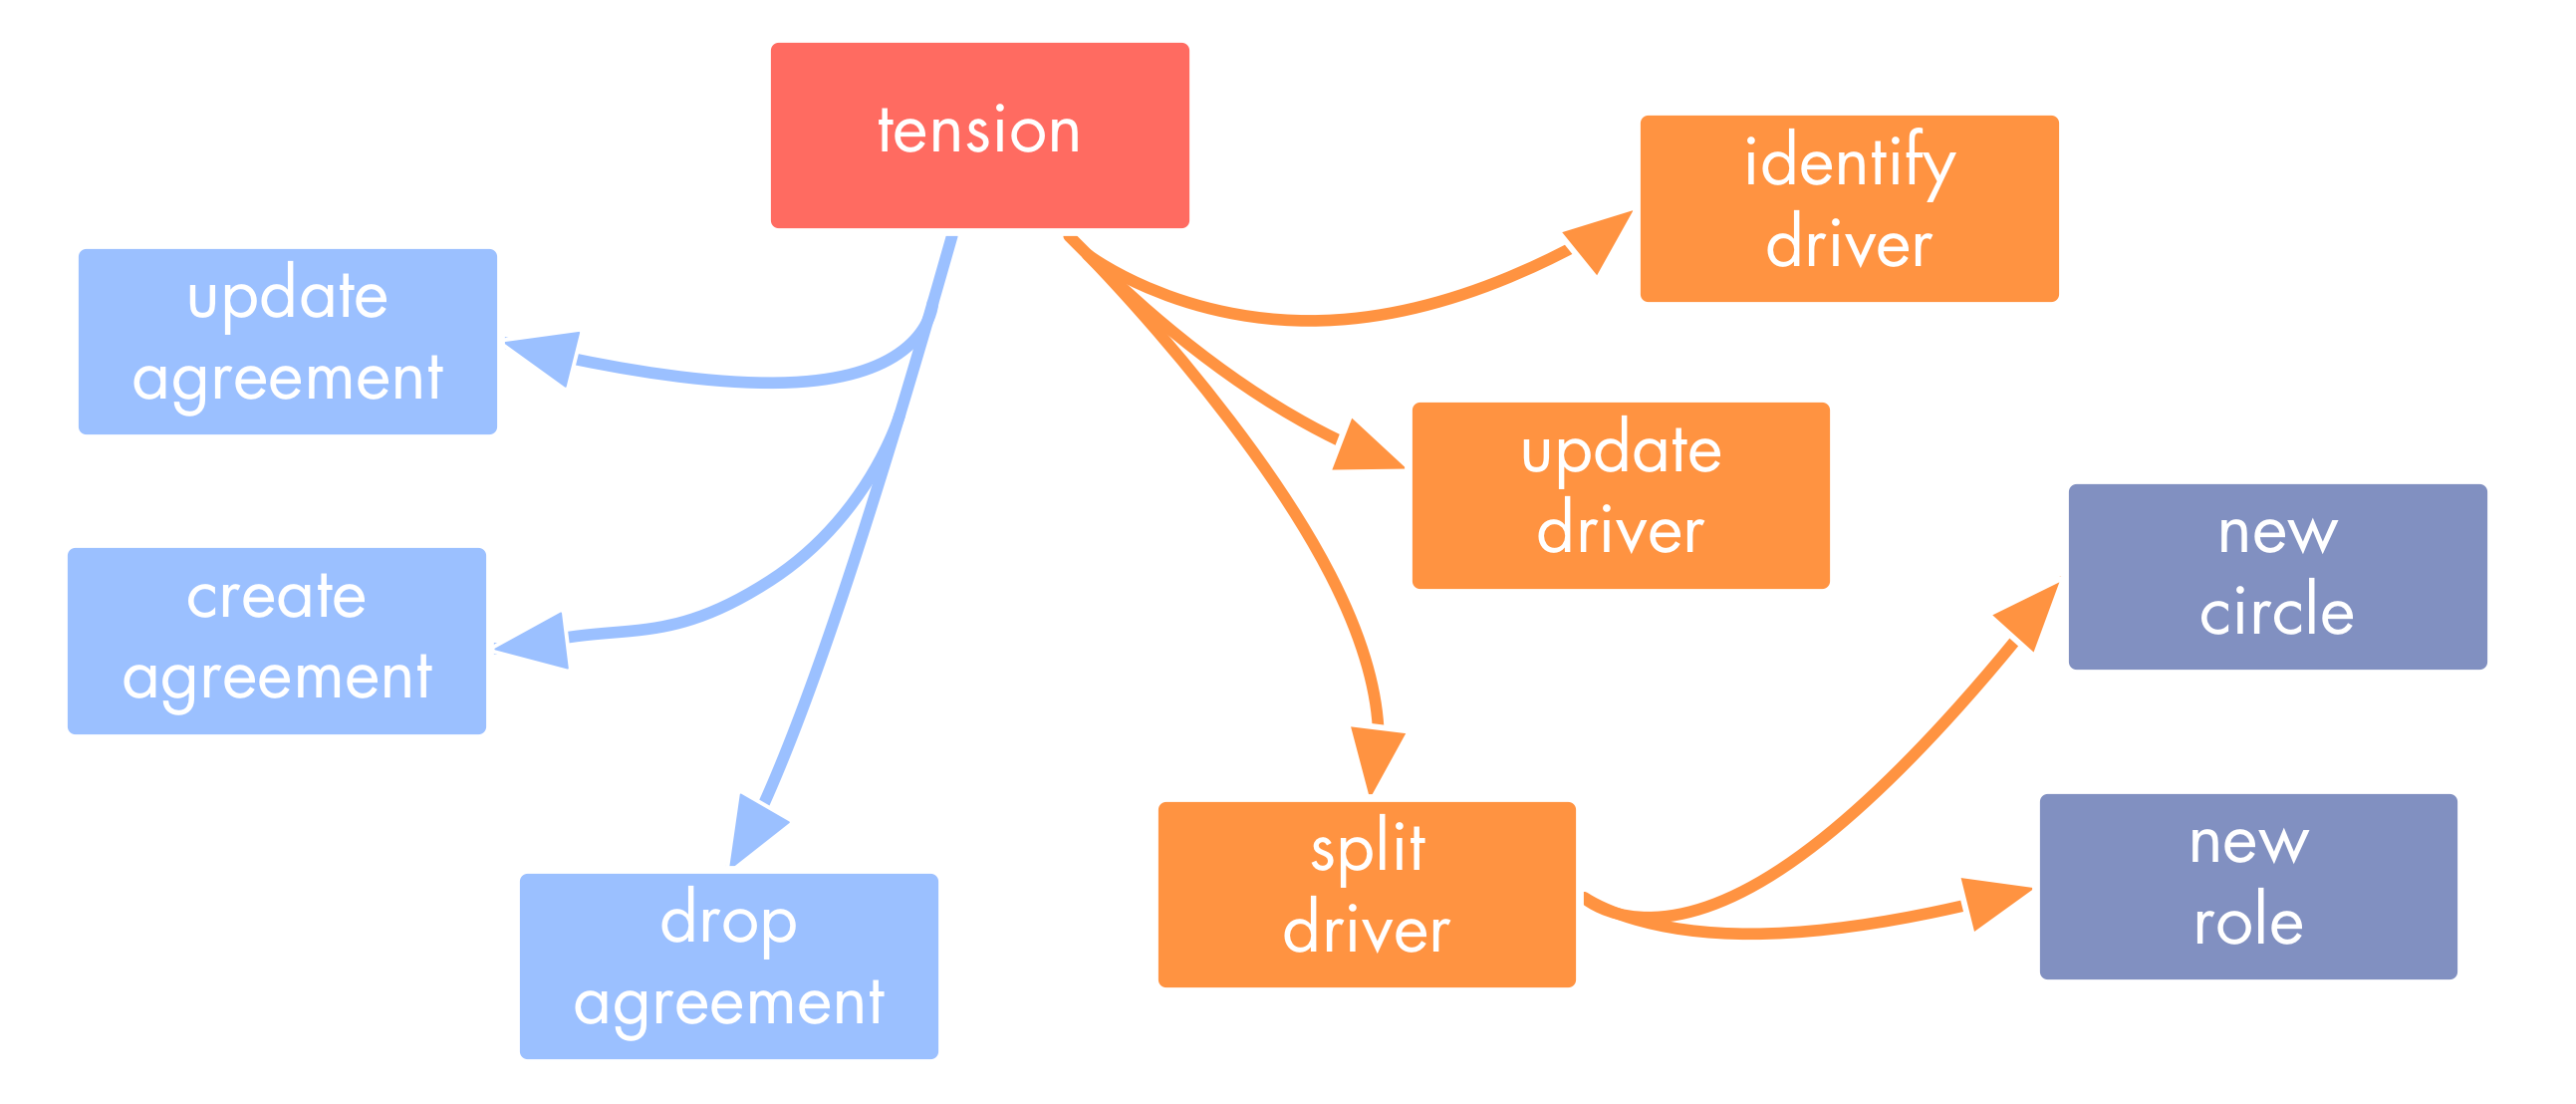
\includegraphics[keepaspectratio,width=\textwidth,height=0.75\textheight]{img/tension-driver-domain/navigate-via-tensions.png}
\end{figure}

\subsection{From Tension to Driver}
\label{fromtensiontodriver}

\begin{itemize}
\item investigating tension leads to the discovery of drivers

\item to identify a possible driver behind a tension we:

\begin{itemize}
\item \textbf{describe} the current reality

\item \textbf{identify} the needs we associate with that reality

\end{itemize}

\item in the process, we resolve some tensions as \textbf{misunderstandings}

\item we validate drivers

\begin{itemize}
\item some tensions are \textbf{outside the domain} we can address

\end{itemize}

\end{itemize}

\chapter{Effective Meetings}
\label{effectivemeetings}

Effective meetings are a cornerstone of effective collaboration and continuous improvement. S3 contains patterns to support you with different aspects of meetings, from preparation (Logbook, Secretary) to the meeting itself (S3 Facilitator, Meeting Facilitation, Rounds, Evaluate Meetings) and beyond (Logbook Keeper and Logbook).

\section{S3 Facilitator}
\label{s3facilitator}

\begin{figure}[htbp]
\centering
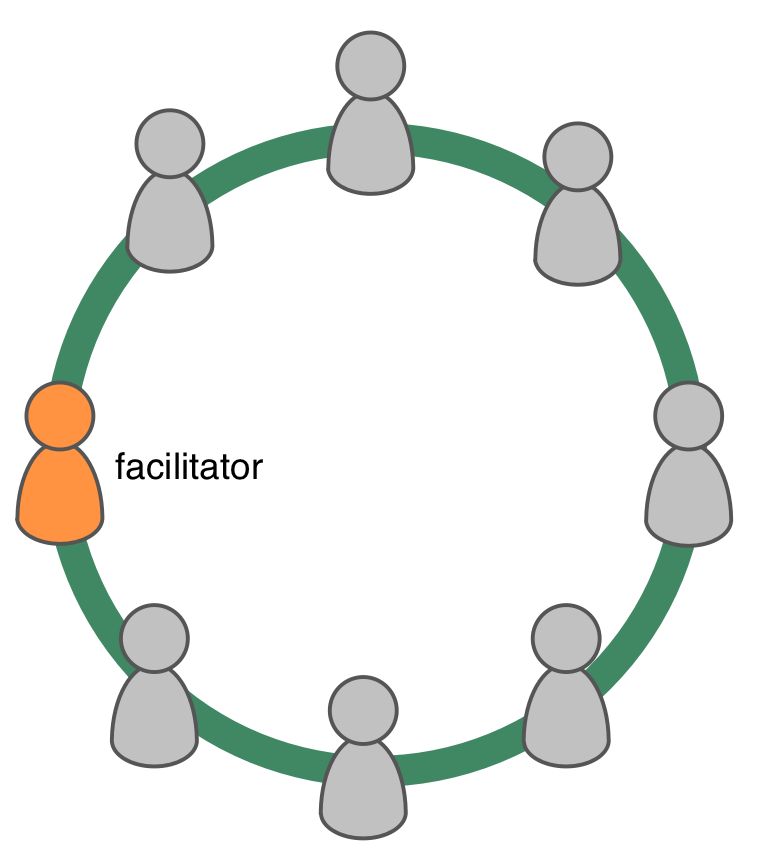
\includegraphics[keepaspectratio,width=\textwidth,height=0.75\textheight]{img/circle/facilitator.png}
\end{figure}

\section{Artful Participation}
\label{artfulparticipation}

A commitment to developing helpful interactions and effective collaboration.

\textbf{Motivation for this pattern}: People wishing to collaborate effectively benefit from identifying, understanding and developing the necessary skills to engage with each other, and with their chosen practices, processes and all agreements they make.

\textbf{Artful participation} is the commitment of an individual to participate in a proactive, coherent and elegant way in all aspects of collaboration in teams and organizations they are a part of.

\subsection{Indicators for using this pattern}
\label{indicatorsforusingthispattern}

\subsubsection{Conditions:}
\label{conditions:}

\begin{itemize}
\item People disengaged or not fully engaged

\item People unsure how to contribute

\item Ineffective participation, despite explicit agreements * Dysfunctional communication

\end{itemize}

\subsubsection{Needs:}
\label{needs:}

\begin{itemize}
\item Effective collaboration

\item Engagement

\item People accountable for their agreements and actions

\item Helpful interactions

\end{itemize}

\subsection{The Details}
\label{thedetails}

Being accountable is a learned skill and while making an agreement may be (relatively) easy, keeping up with the implications is hard: many agreements require discovering necessary skills and developing them.

Intentional commitment to agreements amplifies learning, and the more participants learn about how to support agreements, the more they learn about the agreements themselves.

Intentional effort of participants to support each other makes stronger teams and full engagement makes happy people, better agreements, and closer collaboration.

\subsubsection{Elements of Artful Participation}
\label{elementsofartfulparticipation}

A brief guide for what makes collaboration effective, and how to develop accountability for agreements:

Artful participation is a individual commitment to…

\begin{itemize}
\item actively keeping and following-up on all agreements made, in the best way possible, given the circumstances

\item consciously balancing personal needs with those of a team and the organization as a whole

\item developing the necessary skills to do so

\item supporting others in doing the same

\end{itemize}

Whenever the individual discovers impediments or obstacles to their contribution or to existing agreements, which they can't resolve on their own, they bring them to the attention of everyone involved in the agreement to resolve the problem together.

Although anyone can commit to artful participation on their own, the effect is much greater when a full team or even an entire organization embraces artful participation together.

\subsubsection{Some questions to help with artful participation:}
\label{somequestionstohelpwithartfulparticipation:}

\begin{itemize}
\item How will I support myself and others in participating more artfully?

\item Where are my interactions with others not particularly helpful or effective?

\item Which are the agreements I find hard to keep or contribute to? What can I do to change that?

\item What are skills that would support me in artful participation?

\item What would artful participation mean in relation to{\ldots}

\begin{itemize}
\item {\ldots} my daily activities

\item {\ldots}collaboration and interaction with others?

\item {\ldots}the organization? {\ldots}our clients?

\item {\ldots}the wider environment?

\end{itemize}

\end{itemize}

\subsection{Related Patterns}
\label{relatedpatterns}

\begin{itemize}
\item \emph{Adopt the Seven Principles} provides a powerful guiding framework around artful participation

\item \emph{Agree on Values} supports a team align on their chosen values, which provides both focus and guide for artful participation

\item \emph{Be the Change} is another pattern to support an individual in bringing S3 to their team or organization

\item \emph{Effectiveness Review} provides feedback on one's participation in a role

\item \emph{Meeting Evaluation} supports learning about a group's participation after a meeting

\item Understanding the concept of \emph{Objections} helps to decide when the team needs to evolve an agreement

\item \emph{Qualifying Drivers} is a proactive way of understanding things before bringing them to the team

\end{itemize}

\section{Logbook}
\label{logbook}

\begin{itemize}
\item Organization:

\begin{itemize}
\item driver, strategy

\item organizational values

\item organizational structure

\item agreements

\end{itemize}

\item Circle:

\begin{itemize}
\item driver, strategy

\item agreements

\item role definitions and role improvement plans

\end{itemize}

\item Personal logbooks

\begin{itemize}
\item role descriptions

\item tasks

\item personal strategy and personal policy

\end{itemize}

\end{itemize}

\section{Logbook Keeper}
\label{logbookkeeper}

{\ldots}

\section{Meeting Evaluation}
\label{meetingevaluation}

\begin{figure}[htbp]
\centering
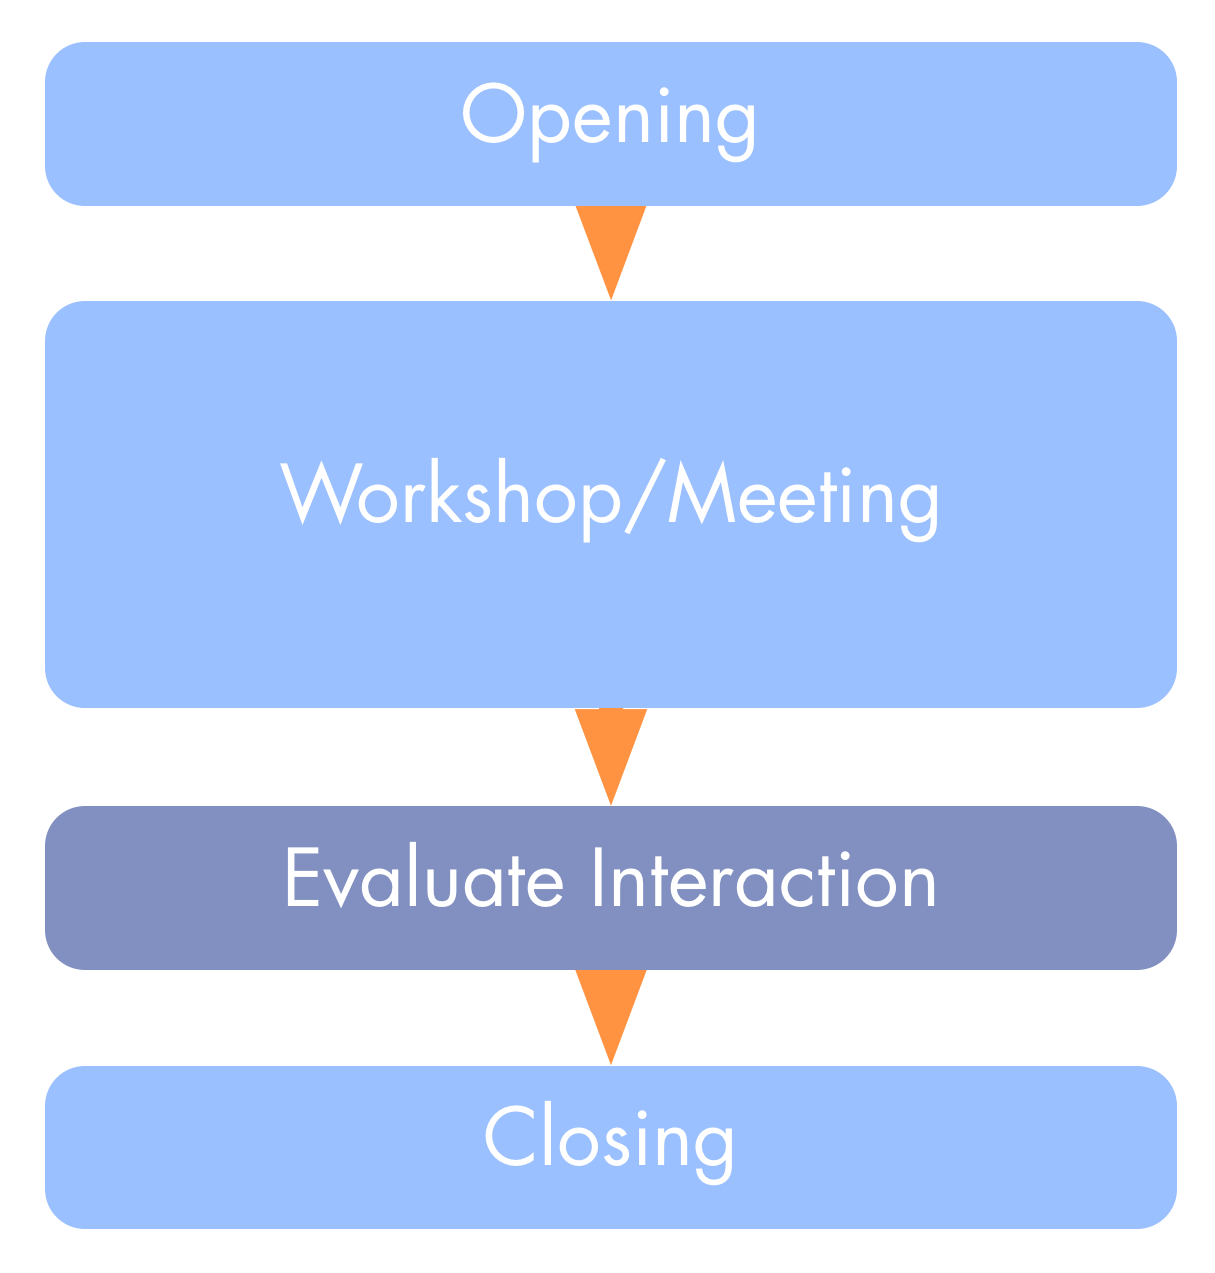
\includegraphics[keepaspectratio,width=\textwidth,height=0.75\textheight]{img/meetings/evaluate-interactions.png}
\end{figure}

\section{Meeting Facilitation}
\label{meetingfacilitation}

When we meet, we want to develop shared understanding, exchange information, learn, and co-create responses to the driver of the meeting. Facilitation keeps meetings and workshops crisp, joyful and effective by

\begin{itemize}
\item giving everyone a voice and thus enabling different perspectives

\item selecting activities to support the development of shared understanding, learning, and solutions

\item supporting the group by mirroring and visualizing what is happening

\item helping the group navigate the agenda in the time available

\end{itemize}

As a facilitator, you would:

\begin{itemize}
\item prepare for the meeting

\begin{itemize}
\item prepare room and materials

\item design the workshop, select activities and interactions for the different phases of the workshop:

\begin{itemize}
\item opening the workshop, ground rules

\item understand driver\slash intended outcome

\item activities to generate insight and develop shared understanding

\item selecting what topics to work on

\item make decisions \slash  action planning

\item evaluate the outcome and learn for the next workshop

\item closing

\end{itemize}

\end{itemize}

\item during the workshop

\begin{itemize}
\item time-box workshop and each activity

\item document process and results in real time

\item navigate the workshop

\end{itemize}

\item after the workshop

\begin{itemize}
\item take photographs of all the artifacts created and share with the group

\end{itemize}

\end{itemize}

\section{Meeting Host}
\label{meetinghost}

{\ldots}

\section{Rounds}
\label{rounds}

A group facilitation technique to maintain equivalence.

\begin{enumerate}
\item Pick a random person to start

\begin{itemize}
\item begin with a different person each time to maintain equivalence

\end{itemize}

\item Go around the circle, give everyone the chance to speak

\end{enumerate}

There's a number of ways that experienced groups can fast track certain rounds.

\begin{figure}[htbp]
\centering
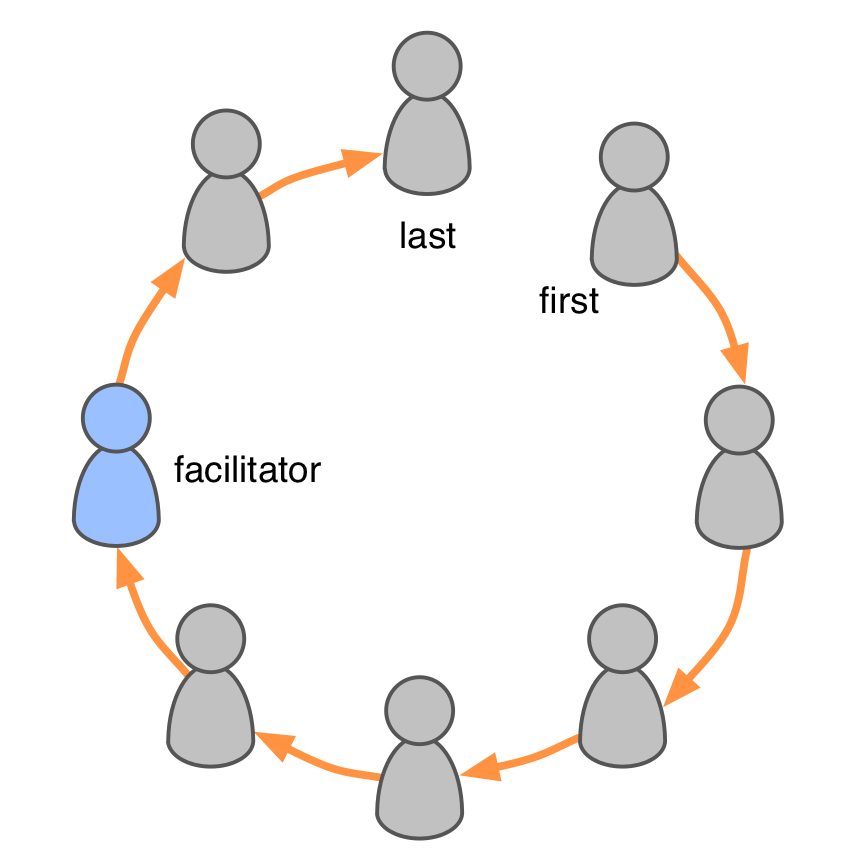
\includegraphics[keepaspectratio,width=\textwidth,height=0.75\textheight]{img/circle/rounds.png}
\end{figure}

\chapter{Coordinating Work}
\label{coordinatingwork}

S3 specifically addresses self-organization through a collection of patterns for coordinating work that go beyond the role of a coordinator or a simple operations meeting.

\section{Coordination Meeting}
\label{coordinationmeeting}

{\ldots}

\section{Coordinator Role}
\label{coordinatorrole}

{\ldots}

\section{Daily Standup}
\label{dailystandup}

A pattern for enabling self-organization.

\{$>$$>$ removed ``in daily activity'', as the standup also enables self-organization beyond daily activity -- Bernhard $<$$<$\}

\textbf{Motivation for this pattern:} Teams need to coordinate work, identify impediments and opportunities, and adapt processes according to changing context.

The \textbf{daily standup} is a short, daily meeting where a team coordinates daily work and identifies impediments and opportunities to improve their work process.

\{$>$$>$ fixed a lot of style: line breaks within paragraphs, line breaks between elements of a list, lists elements beginning with dash and tab instead of asterisk and blank. Other than that, no changes in the text. -- Bernhard $<$$<$\}

\subsection{The details}
\label{thedetails}

For the daily standup, the team gathers around a task board every day at the same time, and makes decisions about how to move forward with their work items.

It's helpful to appoint a facilitator to keep the meeting on task and within time (if possible under 15 minutes).

The facilitator facilitates quick decisions on the spot and identifies discussions and decisions requiring more time, to be scheduled after the standup, or added to a backlog to process later.

Daily standups enable teams to

\begin{itemize}
\item make quick decisions about work using the knowledge of the whole team

\item rapidly identify impediments and respond as needed

\item accelerate learning

\item improve their work processes as required

\end{itemize}

There are two common patterns for daily standups, one is \textbf{value focussed}, the other one is \textbf{people-focused}.

\subsubsection{Value-focused standup}
\label{value-focusedstandup}

The \emph{value-focused standup} helps a team focus on effectively collaborating on the most valuable work items.

In this approach, the facilitator points out the most valuable work item on the board (often the one closest to the upper right corner of the board), and asks the team members: \textbf{``How can we move this item forward?''}

Team members can volunteer to contribute to that work item, and then the facilitator moves to the next item, and so on, until the circle members cannot pull in more work for the day.

Impediments or blocked items can be discussed during or after the standup.

\subsubsection{People-focused standup}
\label{people-focusedstandup}

Team members answer three questions in a round:

\begin{itemize}
\item What did you do yesterday?

\item What are you going to do today?

\item What stands in your way?

\end{itemize}

The facilitator supports people to be brief and to the point, making a note of all impediments mentioned in order to make sure they are addressed - either by scheduling brief discussions after the standup, or by adding them to a backlog.

The \emph{people focused standup} is helpful when each team member mostly works in their own silo and tasks are not commonly shared.

Team members are constantly up to date with the state of the team's work and get the opportunity for contributing to other people's tasks when there's a bottleneck.

Over time this approach might translate into improvements for closer collaboration, with a team finally adopting the \emph{value-focused standup} (above).

\subsubsection{Iterations or Continuous Flow}
\label{iterationsorcontinuousflow}

Teams working on products often use an iterative approach, planning work in regular intervals lasting for a certain period of time (the iteration). Other teams work from a prioritized backlog and hold planning sessions as needed. Teams delivering ongoing services often work without explicit planning.

The daily standup can be combined with any of these approaches and can benefit all types of work process.

\begin{figure}[htbp]
\centering
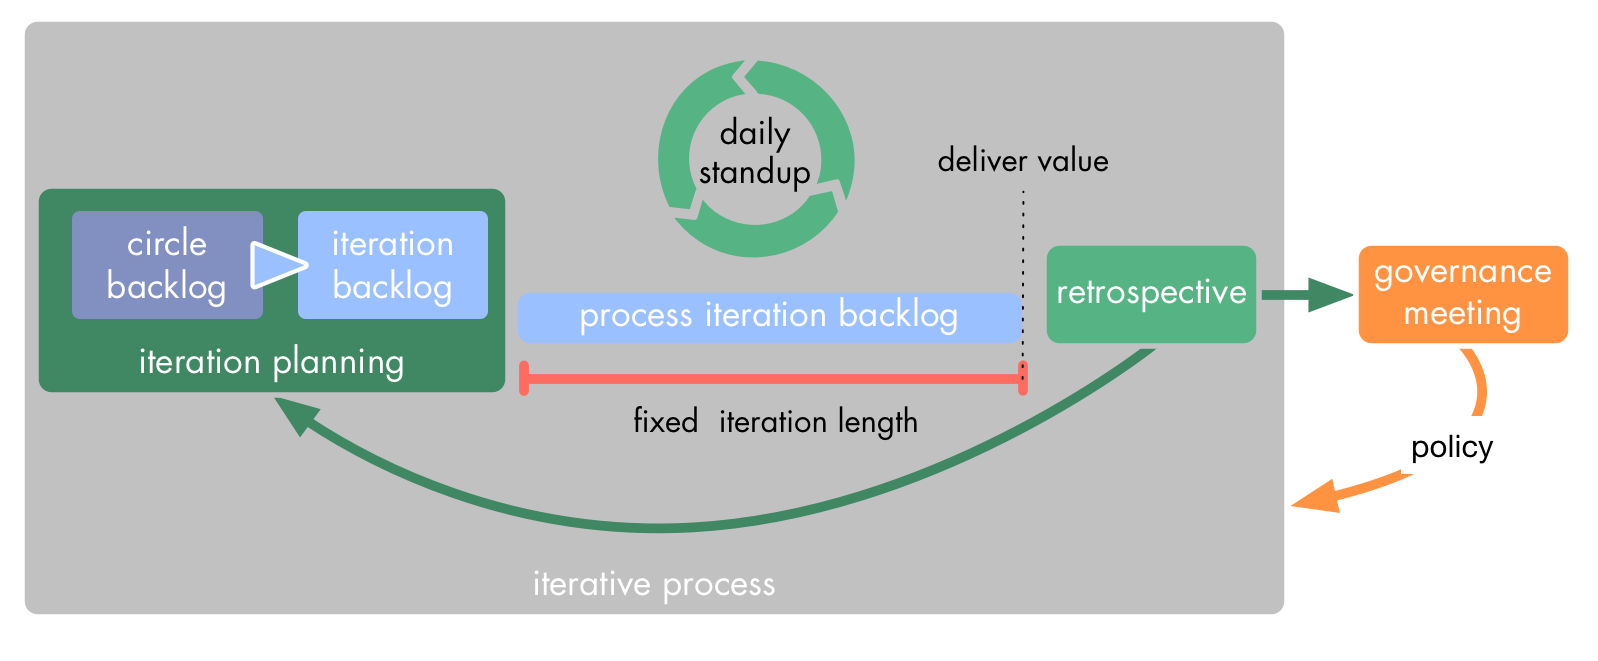
\includegraphics[keepaspectratio,width=\textwidth,height=0.75\textheight]{img/meetings/iterations.png}
\caption{Daily Standup and Continuous Flow}
\end{figure}

\begin{figure}[htbp]
\centering
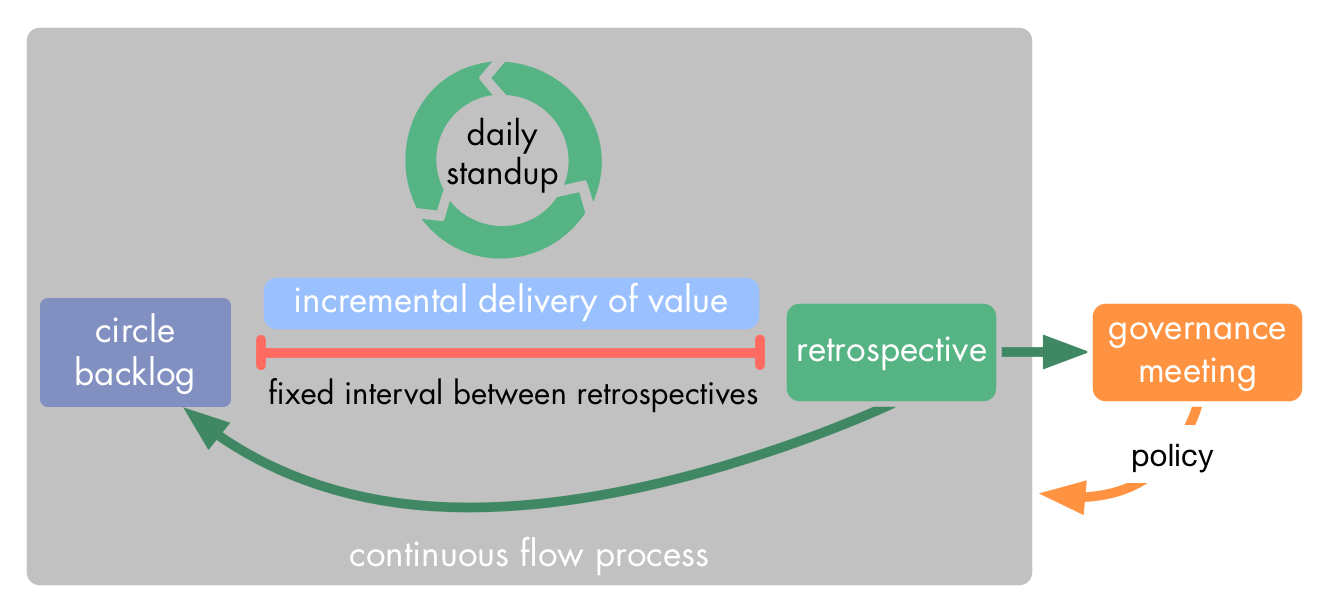
\includegraphics[keepaspectratio,width=\textwidth,height=0.75\textheight]{img/meetings/continuous-flow.png}
\caption{Daily Standup and Iterations}
\end{figure}

\subsection{Related Patterns}
\label{relatedpatterns}

\emph{Coordinating work} - Another way to coordinate daily activity is through assigning the function of coordination to the \emph{Coordinator Role}, \emph{Coordination Circle}.

\emph{Coordination meeting} for synchronizing, organizing and aligning daily workflow within and across teams.

\emph{Organizing in Circles} of semi-autonomous teams

Some content from daily standups inform the \emph{Planning and review meetings}

Work items can be visualized (\emph{Visualize Work}) in a \emph{Prioritized Backlog}, and can be dealt with through a \emph{Pull System for Work}.

\section{Planning And Review Meetings}
\label{planningandreviewmeetings}

When working on products or larger projects that will take weeks or even months to finish, it's often helpful to break them down into smaller parts in order to effectively manage both work itself and expectations of stakeholders.

These parts are commonly called \emph{milestones}, which usually take more than an month to achieve, and whose duration usually extends until work is finished, or \emph{iterations}, which are fixed in duration (usually 1--4 weeks), unfinished items are handed over to the next iteration.

At the beginning of the milestone or iteration there is a \emph{planning meeting} where the circle decides on the timeframe and on how much work to pull in for that period. It's helpful to timebox the meeting to just a few hours, and prepare a prioritized product or project backlog with the topmost items already estimated by the circle.

During the planning session, value, risk and dependencies between work items are discussed, work items are estimated, and, if time allows, broken down into small tasks that can be executed independently. For a successful milestone or iteration, circles often identify a theme, topic or goal, and select work items accordingly.

In the \emph{review meeting} at the end of the iteration or milestone, the circle inspect the results,
sometimes bringing in external stakeholders, the output of the review meeting is fed back into the next planning meeting.

\begin{figure}[htbp]
\centering
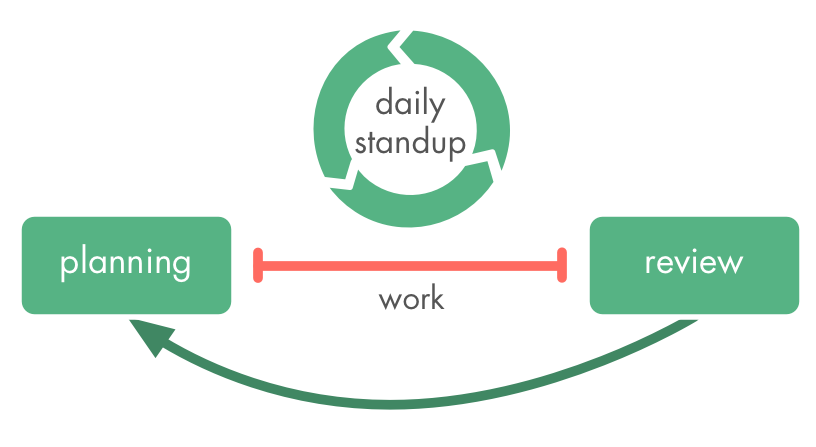
\includegraphics[keepaspectratio,width=\textwidth,height=0.75\textheight]{img/meetings/planning-review-standup.png}
\end{figure}

\section{Prioritized Backlog}
\label{prioritizedbacklog}

When work extends a certain complexity, we need way of identifying what to focus on now, and what can be dealt with later, and at the same time being sure nothing slips to the cracks.

One way to do this is through maintaining a \emph{Prioritized Backlog}, a list of all the uncompleted work and other matters needing to be dealt with need, the most important bits on top. That it's easy to pull in new work when there's capacity: simply take the topmost item you're confident you can work on.

\subsection{Benefits}
\label{benefits}

There's multiple benefits to a prioritized backlog:

\begin{itemize}
\item when pulling in work, we know that we need to pull from the top of the backlog, so the choice is easy and frictionless

\item when we see that we are repeatedly unable to pull from the top, this is a strong indicator of a need to reorganize work processes, development of new skills, and maybe even a new mindset

\item agreeing on work items and prioritization is helpful for developing shared understanding about what needs to be done and how to best approach it

\item prioritization enables us to optimize the value we create by working on the most important things first

\item also, priorization helps reduce the cost of change by enabling just-in-time specification, we only talk about the details of what needs to be done when we're close to actually starting work, so we can avoid discussing detail of less important or less urgent work items which might change again before we can even begin working on it.

\end{itemize}

\subsection{Implementation}
\label{implementation}

For collocated circles a backlog can be crated with sticky notes on a wall, or with index cards (A5 or A5 recommended) and magnets on a whiteboard. There's also many ways of implementing a digital backlog, from Excel or Google Spreadsheets, to generic tools like digital whiteboards or task planning systems, to dedicated backlog tools. It's a good idea to use the simplest tool that does the job for you. Often the minute details about work items do not need to be tracked in the backlog, if necessary we can use a reference number or a link to point us to another location, e.g. a Google Document, a Trello card, or in page in a Wiki.

Things you need to track in the backlog:

\begin{itemize}
\item a \textbf{unique reference numbe}r for each work item, so you can reference the item in other documents or systems

\item a \textbf{title or short description} of the work item

\item the \textbf{order of work items}

\item \textbf{dependencies}: other work items this item is dependent on or related to

\item a \textbf{due date}, e.g. delivery date agreed on with an external party, or a date where the work item will begin to lose value rapidly (e.g. two weeks before christmas for a christmas special). Many items do not have a due date.

\item (optional) a measure for \textbf{value}

\item (optional) a measure for \textbf{investment} (often an estimate of time or complexity)

\end{itemize}

\subsection{Limitations}
\label{limitations}

Priorization requires making tough choices, and some teams are not yet ready to make them: if a team repeatedly considers two or more items as being ``of equal importance'', and can not agree on a default order for these cases, the backlog will fall short on helping the team deliver the most valuable items first.

\section{Pull-System For Work}
\label{pull-systemforwork}

In a pull-system, people or circles pull in new work when they find they have capacity. The opposite would be a push-system, where work items are assigned from a third party.

A pull-system will shift from optimization of capacity - which makes an organization vulnerable to the effects of unforeseen circumstances - towards optimization for throughput, building resilience and organizational agility.

A pull system fosters self-organization, because those who do the work make the call when to build the fence and when to chase the cattle. Since the system is no longer optimized for running on full capacity, people are free to use the now available ``slack time'' for investments in infrastructure, evolution of work processes, and building new skills.

\subsection{Creating a Pull-System}
\label{creatingapull-system}

In order to create a pull-system, both trust and transparency are necessary to empower everyone to be able to contribute effectively. This does not only affect those doing the actual work, who now need access to all information they need to make the right choices when pulling in work, but also ``external'' stakeholders or customers, who now, instead of pushing work items, need to learn a different way of communicating their requirements, and who might also need transparency about the state of work items and projects.

S3 contains many patterns to help with that, here's a selection:

\begin{itemize}
\item \emph{Those Affected Decide} to hand over responsibility for work process to the ones doing the work

\item \emph{Consent Decision Making} and \emph{Proposal Forming}: to use all information available for effectively creating and evolving the agreements which guide pulling in work, such as priorities, plans, contracts etc.

\item \emph{Visualize Work} makes available the information what needs to be done and what is the current state of work

\item in the \emph{Daily Standup}, a team or circle can collaborate on pulling in work

\item a \emph{Prioritized Backlog} makes the choice about which work items to pull in much easier, as do \emph{Planning and Review Meetings}

\end{itemize}

\subsection{Limitations}
\label{limitations}

In a low-trust environment, it will be difficult to establish a pull system, as a pull-system requires trust, first in the ability of people to pull in work items appropriate to the context at hand, and second in the ability and willingness of people to use slack time productively, to the benefit of the organization. What is often overlooked is that also the people need to build trust that a pull-system is not merely a new way for setting up competition.

In these circumstances, trust can be built through first implementing the patterns \emph{Those Affected Decide}, which brings those who used to push work together with those who now will pull, and learn to understand each other's perspective while creating agreements as peers. This is best done in combination with \emph{Proposal Forming} and \emph{Consent Decision Making}.

\section{Retrospective}
\label{retrospective}

\textbf{Reflect on a longer period of work and improve agreements.}

\begin{itemize}
\item \ensuremath{\sim}60 min

\item cadence, usually 2--4 weeks

\item helps seeing the bigger picture, and identifying more complex types of waste

\item What can we learn from the last iteration of work?

\item Are our tools still sharp enough?

\item Are we still going in the right direction?

\end{itemize}

\textbf{Building in continuous improvement of process:}

\begin{itemize}
\item goal: reflection on the past to guide process improvement

\item output: proposals for agreements, tensions, drivers or tasks

\item facilitated meeting (\ensuremath{\sim}1hr)

\item regular intervals (1--4 weeks)

\item adapt to situation and context:

\begin{itemize}
\item 5 phases with many different patterns for each phase

\end{itemize}

\end{itemize}

\subsection{A time to reflect on process improvement}
\label{atimetoreflectonprocessimprovement}

\begin{figure}[htbp]
\centering
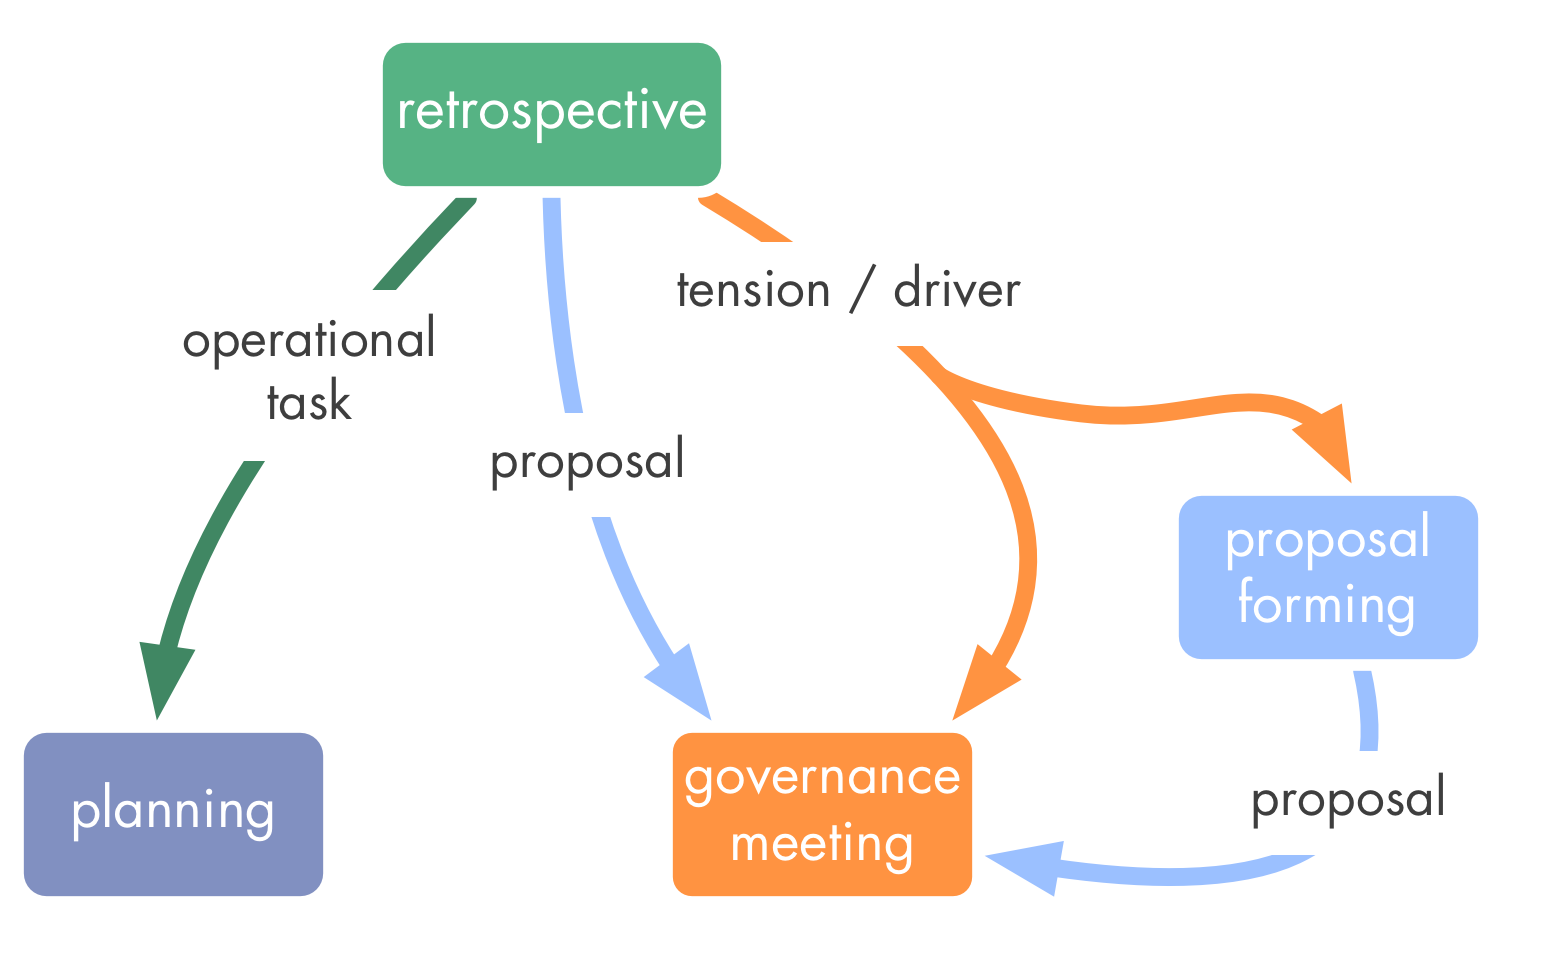
\includegraphics[keepaspectratio,width=\textwidth,height=0.75\textheight]{img/meetings/retrospective.png}
\end{figure}

\subsection{5 Phases of a Retrospective Meeting}
\label{5phasesofaretrospectivemeeting}

\begin{enumerate}
\item Set the Stage

\item Gather Data

\item Generate Insights

\item Decide What to Do

\item Close the Retrospective

\end{enumerate}

Activities for each phase can be found at \href{http://www.plans-for-retrospectives.com/}{plans-for-retrospectives.com}\footnote{\href{http://www.plans-for-retrospectives.com/}{http:/\slash www.plans-for-retrospectives.com\slash }}

\begin{figure}[htbp]
\centering
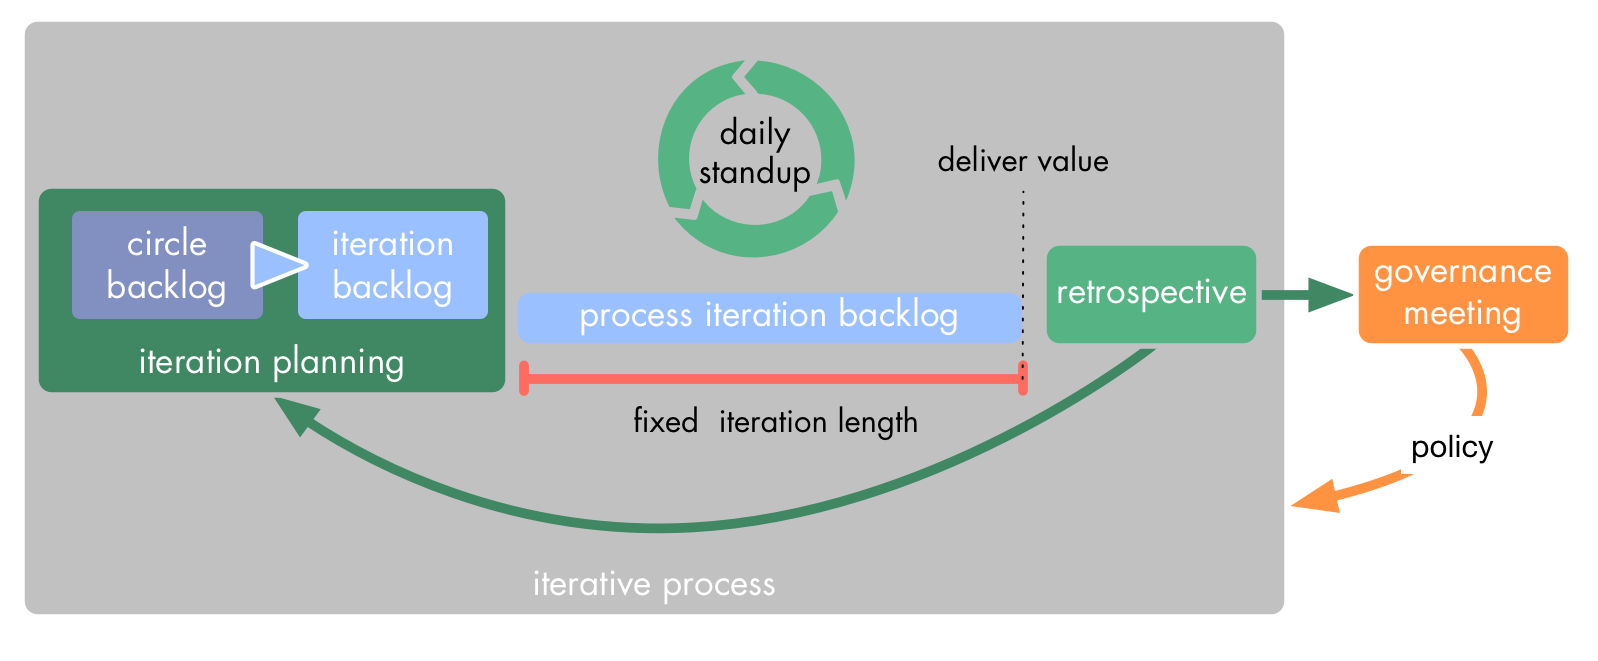
\includegraphics[keepaspectratio,width=\textwidth,height=0.75\textheight]{img/meetings/iterations.png}
\caption{Retrospective and Continuous Flow}
\end{figure}

\begin{figure}[htbp]
\centering
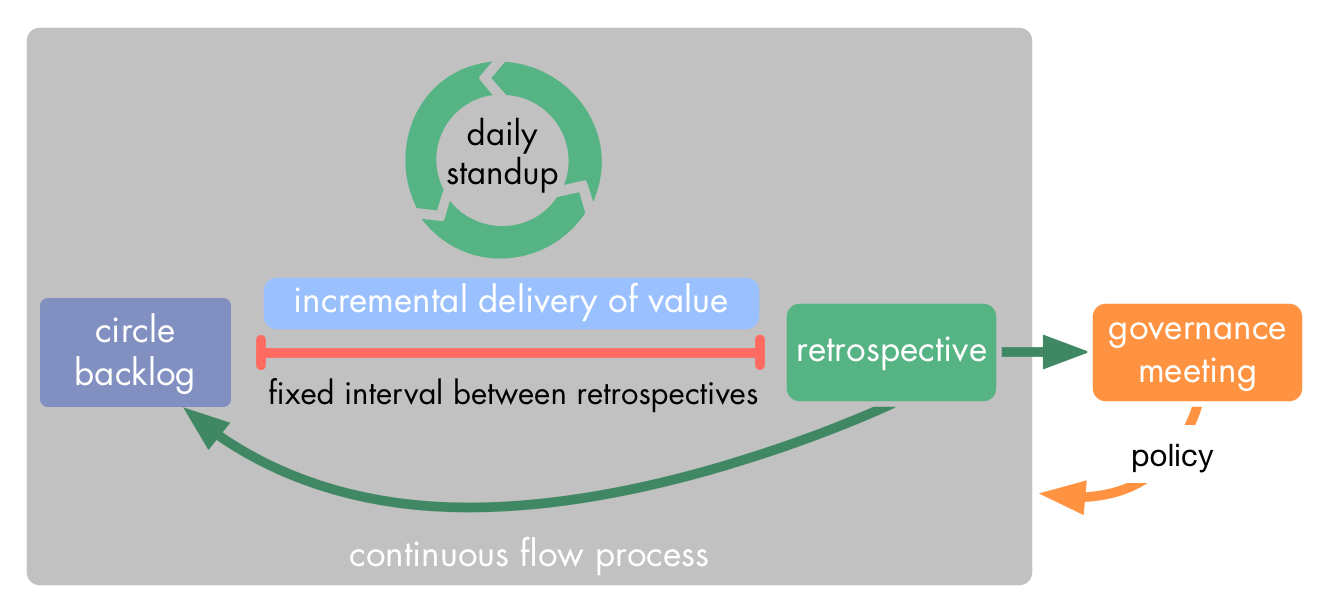
\includegraphics[keepaspectratio,width=\textwidth,height=0.75\textheight]{img/meetings/continuous-flow.png}
\caption{Retrospective and Iterations}
\end{figure}

\section{Visualize Work}
\label{visualizework}

In order to empower a circle for self-organization, we need to make transparent both the agreed upon work process and the state of all work items currently in planning, in progress or completed transparent. Only if all work items are visible to all circle members, people can pull in work when they have capacity, instead of work being pushed by a coordinator.

Collocated teams can do this with post-its on a wall, or with index cards and magnets on a white board. Distributed teams can use an ever increasing number of apps available for this use case , from generic tools like Google Spreadsheets or digital whiteboards, to task management systems for teams (e.g. Asana, Todoist) or dedicated apps for task boards (Trello, Kanbanery, Leankit). Many teams use both a digital system and a card wall, and synchronize them once a day, commonly around the daily standup.

When visualizing work, first try to identify what different types of work items you have, e.g. customer request, project tasks, reporting tasks, rework. Decide whether or not it is necessary to distinguish between these types of work items, and how you are going to make that visible on your board, will you use colors, or symbols, or highlights? Are there different priorities, expedite items that take priority, and if so, how do you express ?

Then figure out what stages these work items go through, like ``to do'', ``in progress'', ``review'' and ``done''. At this stage, simply visualize what you're doing already, don't make any changes to your process. You might end up with a very simple layout, or something rather complicated. Implement the layout in the system you thinks makes the most sense for you now, on a wall, or with software.

If you have any agreements guiding your workflow, e.g. which items have priority over others, or what is necessary for an item to move forward, quality standards and the like, it's a good idea to make them visible next to your board, so you can get together and review, discuss and update these agreements to improve the flow of items through your board.

\chapter{Building Organizations}
\label{buildingorganizations}

Patterns for growing an organization along the principles behind S3. In the addition to the patterns in this sections there's also two subsections: Patterns for People and Roles, and patterns for Organizational Structure.

\section{Align Flow}
\label{alignflow}

\subsection{Flow of Value}
\label{flowofvalue}

\begin{itemize}
\item flow of value is guided by agreements (explicit and implicit), and assumptions

\item work in progress is considered waste as it ties up resources

\item continuous flow of value prevents accumulation of waste

\begin{itemize}
\item it also makes for shorter feedback loops and amplifies learning

\end{itemize}

\end{itemize}

\subsection{Flow of Value and Flow of Information}
\label{flowofvalueandflowofinformation}

\begin{figure}[htbp]
\centering
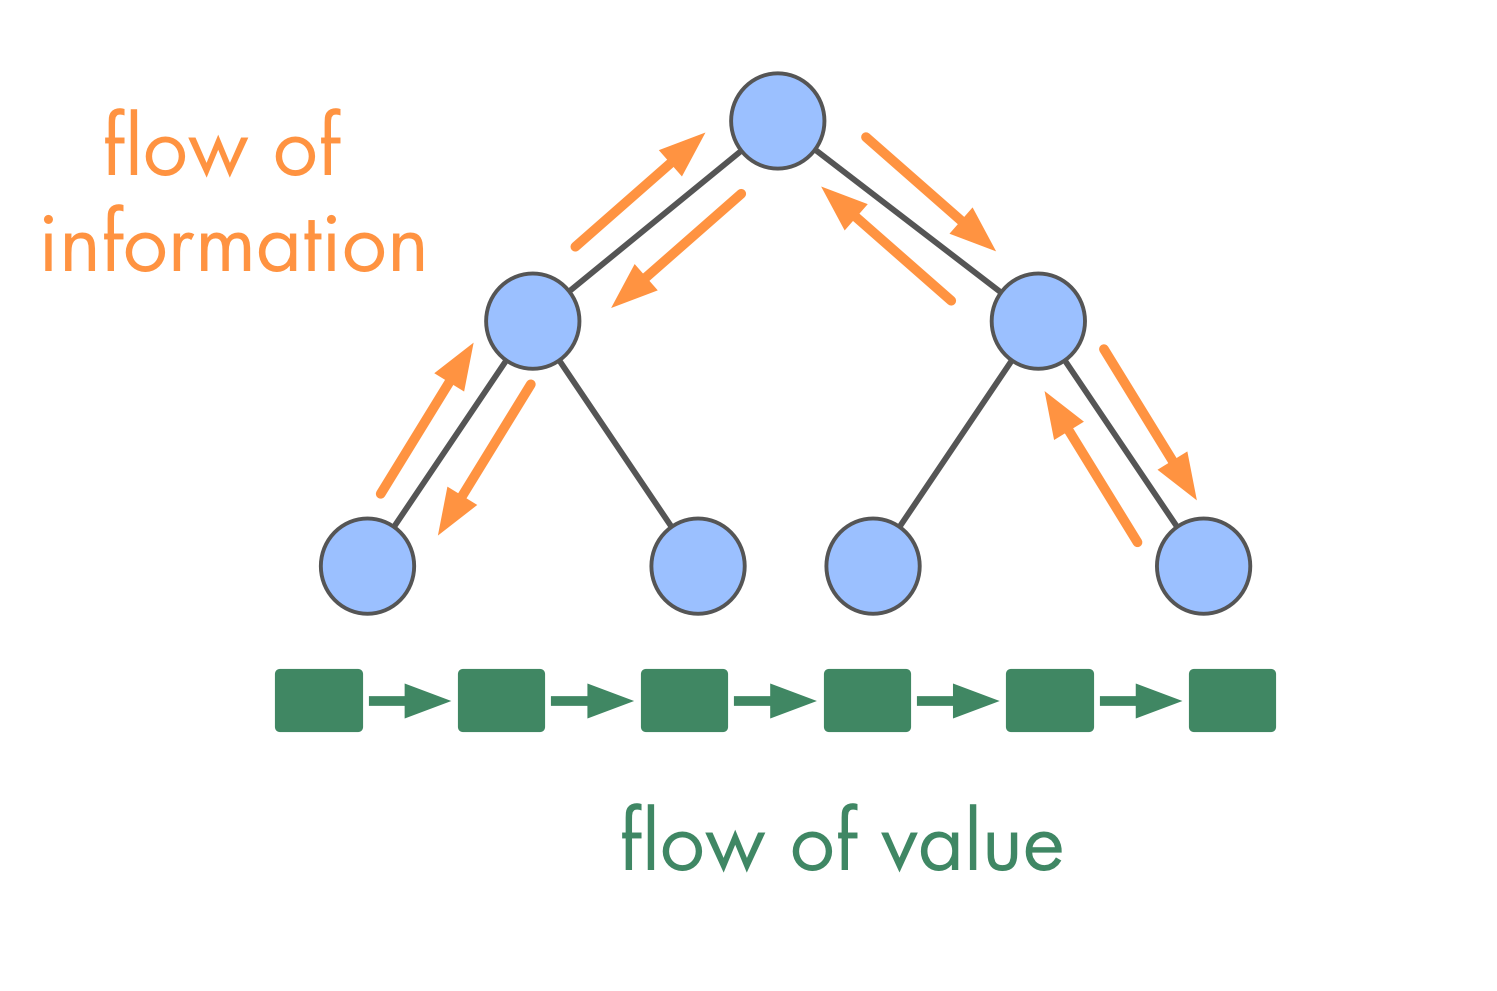
\includegraphics[keepaspectratio,width=\textwidth,height=0.75\textheight]{img/workflow-and-value/types-of-flow.png}
\end{figure}

\begin{itemize}
\item in an effective organization, the \textbf{flow of information and influence supports the continuous flow of value}

\item alignment is achieved and maintained through continuous improvement of agreements

\end{itemize}

\section{Open Systems}
\label{opensystems}

{\ldots}

\section{Organize in nested domains}
\label{organizeinnesteddomains}

{\ldots}

\chapter{People and Roles}
\label{peopleandroles}

\begin{figure}[htbp]
\centering
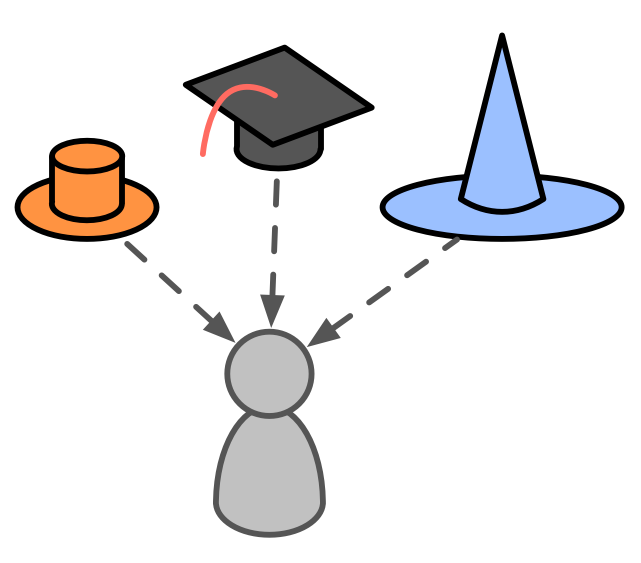
\includegraphics[keepaspectratio,width=\textwidth,height=0.75\textheight]{img/people-and-roles/roles.png}
\end{figure}

\section{People, Functions and Roles}
\label{peoplefunctionsandroles}

\begin{itemize}
\item identify functions required to respond to a driver

\item if a function is best addressed by a role:

\begin{itemize}
\item define the role

\item select people for the role

\item support development of people in the role

\end{itemize}

\end{itemize}

\section{Role Definition and Improvement}
\label{roledefinitionandimprovement}

\begin{figure}[htbp]
\centering
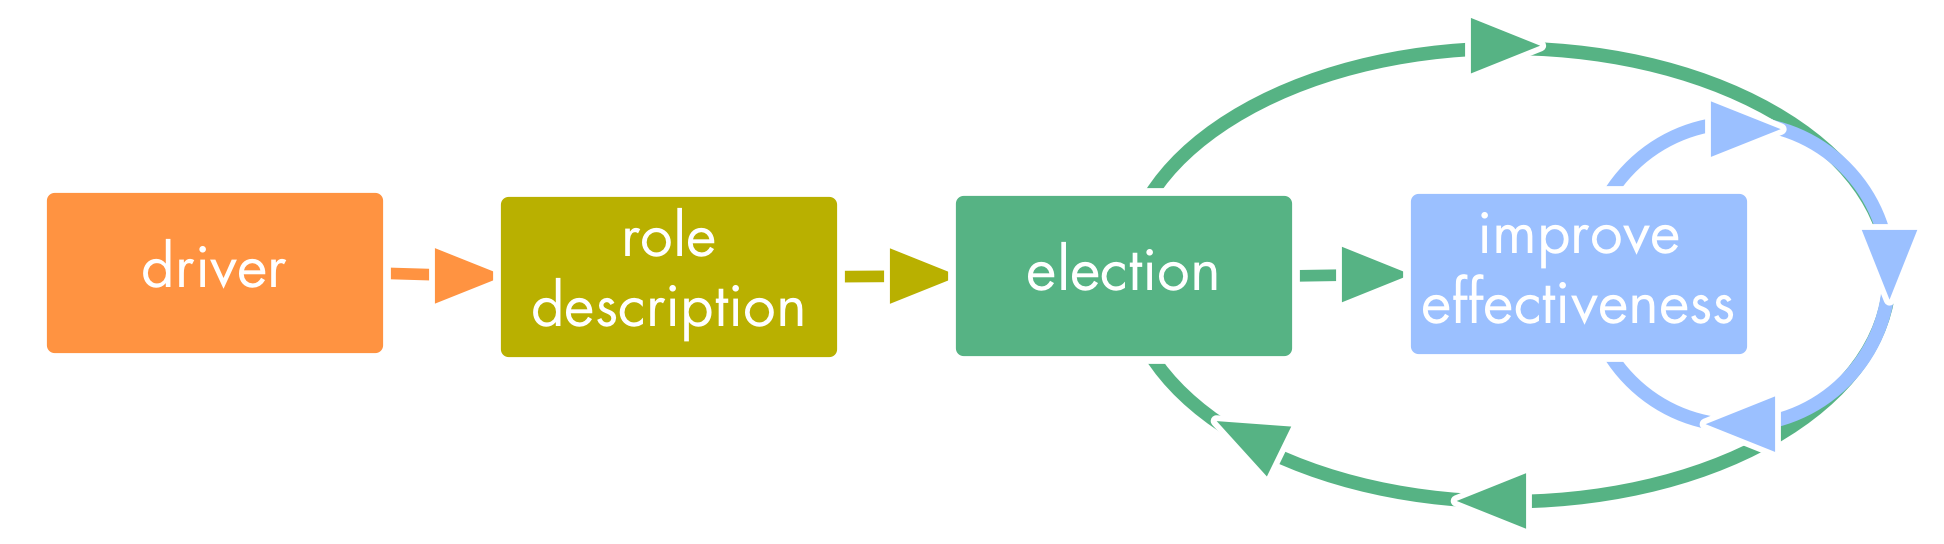
\includegraphics[keepaspectratio,width=\textwidth,height=0.75\textheight]{img/people-and-roles/role-improvement.png}
\end{figure}

\section{Performance Improvement Process}
\label{performanceimprovementprocess}

Continuous improvement of the effectiveness of people in roles \#\#

\begin{enumerate}
\item Conduct effectiveness review

\item Create development plan

\item Full circle consents to development plan

\item Act on the plan

\end{enumerate}

\begin{figure}[htbp]
\centering
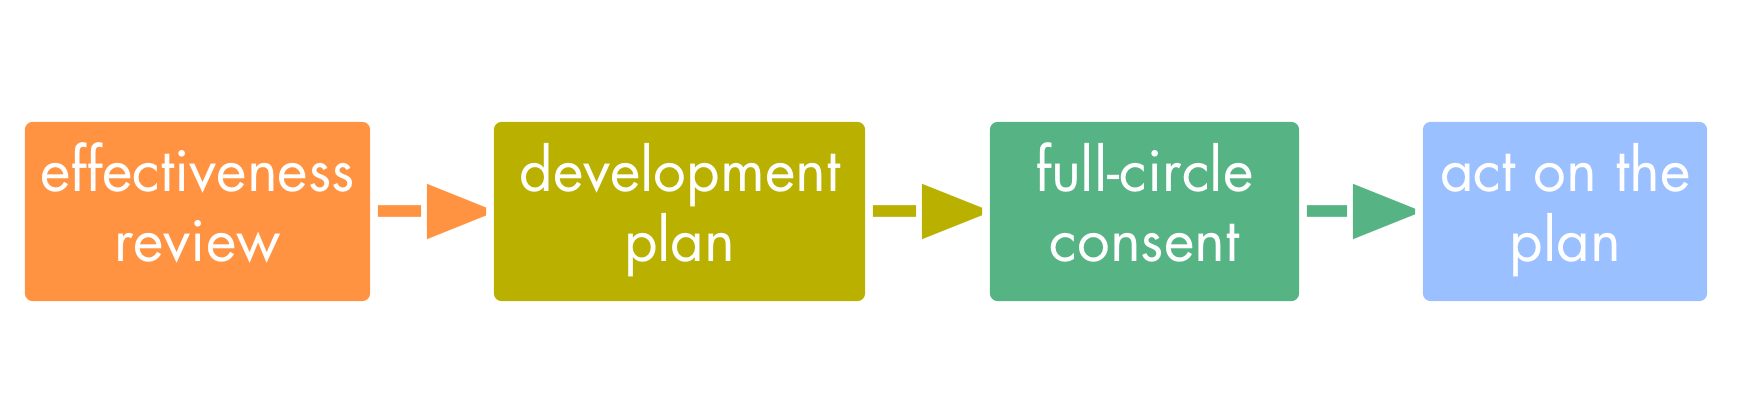
\includegraphics[keepaspectratio,width=\textwidth,height=0.75\textheight]{img/people-and-roles/performance-improvement-process.png}
\end{figure}

{\ldots}

\section{Development Plan}
\label{developmentplan}

\textbf{Contents:}

\begin{itemize}
\item current role description

\item appreciations

\item areas for improvement

\item action items to improve effectiveness

\item evaluation criteria

\item suggested amendments to role description

\end{itemize}

\section{Effectiveness Review}
\label{effectivenessreview}

\begin{itemize}
\item a process to harvest appreciations, identify opportunities for improvement and evolve the role

\item the individual holding the role initiates the process and begins each step

\end{itemize}

\subsection{Steps}
\label{steps}

\begin{enumerate}
\item Invite people with complementing perspectives to contribute to the review, and a facilitator

\item Collect appreciations

\item Identify areas for improvement

\begin{itemize}
\item personal development

\item updates to role description, function or driver

\end{itemize}

\item Co-create and consent to a development plan

\end{enumerate}

\begin{figure}[htbp]
\centering
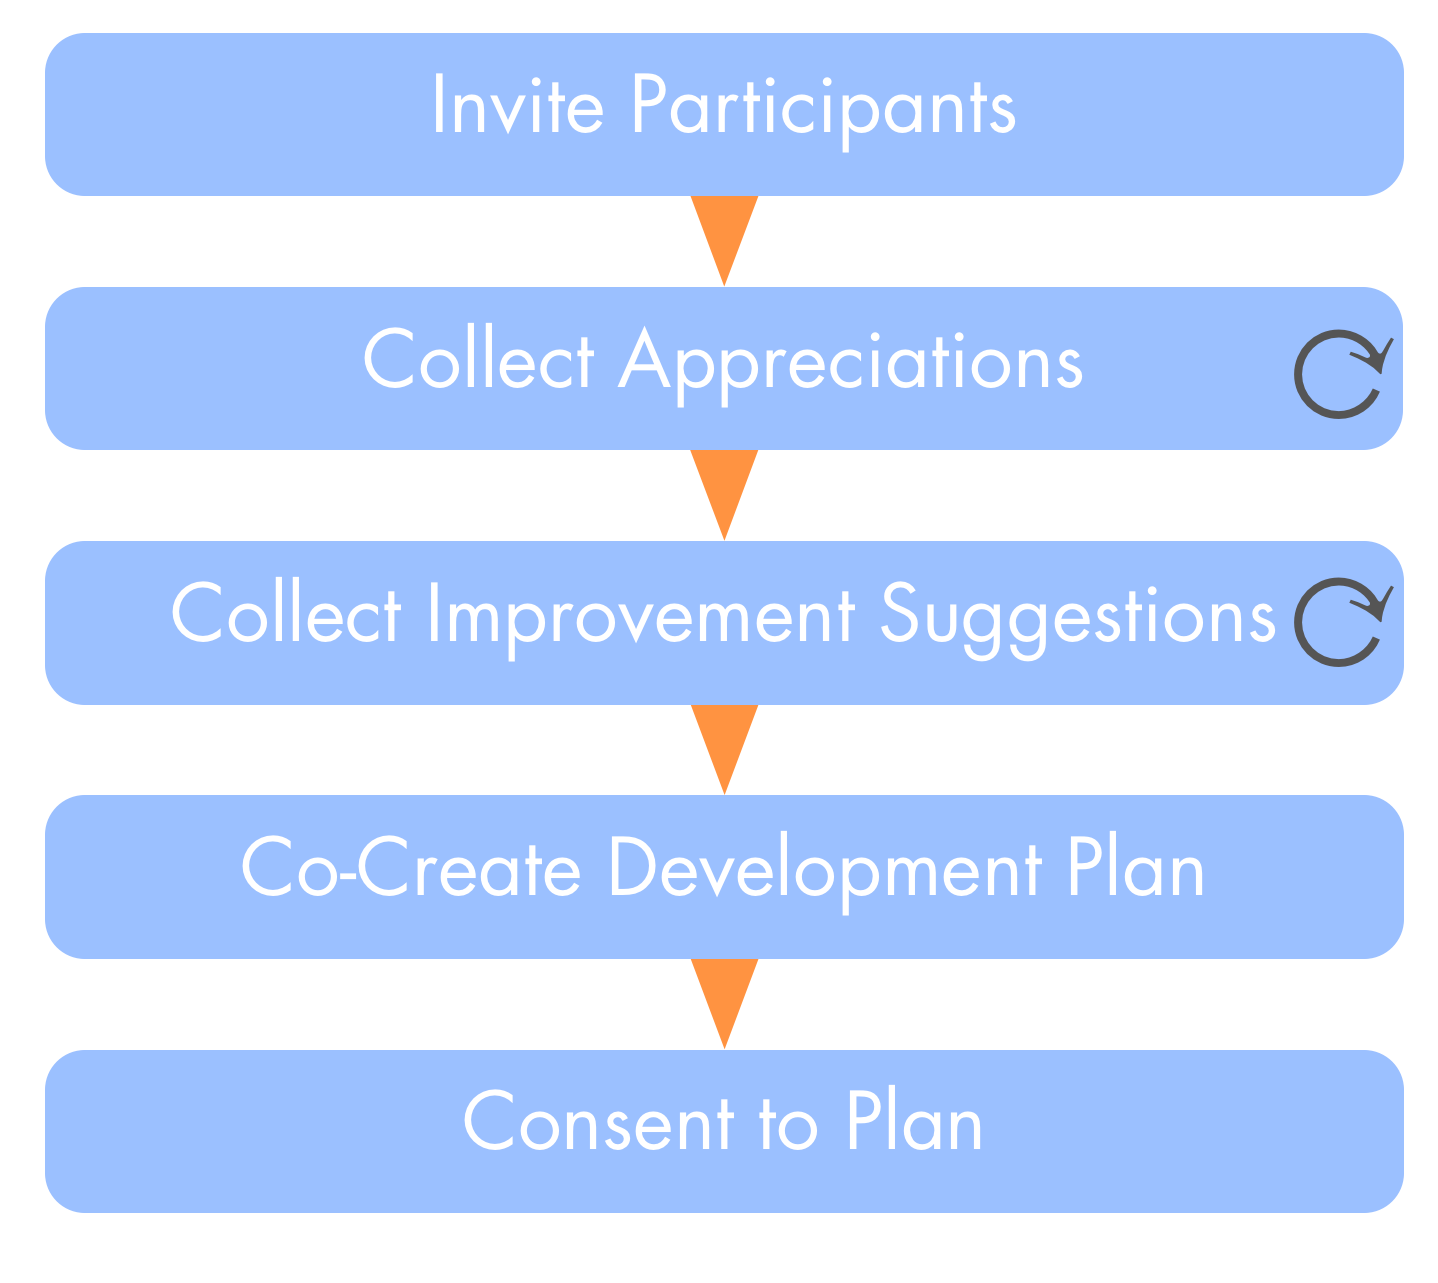
\includegraphics[keepaspectratio,width=\textwidth,height=0.75\textheight]{img/people-and-roles/effectiveness-review.png}
\end{figure}

\section{Role}
\label{role}

{\ldots}

\section{Role Description}
\label{roledescription}

\begin{itemize}
\item role descriptions can be created using proposal forming

\item a minimal role description contains:

\begin{itemize}
\item driver

\item term

\item key responsibilities

\item preferable skills, experience and qualities

\item cadence of effectiveness reviews

\end{itemize}

\end{itemize}

\subsection{Template for Role Descriptions}
\label{templateforroledescriptions}

\begin{figure}[htbp]
\centering
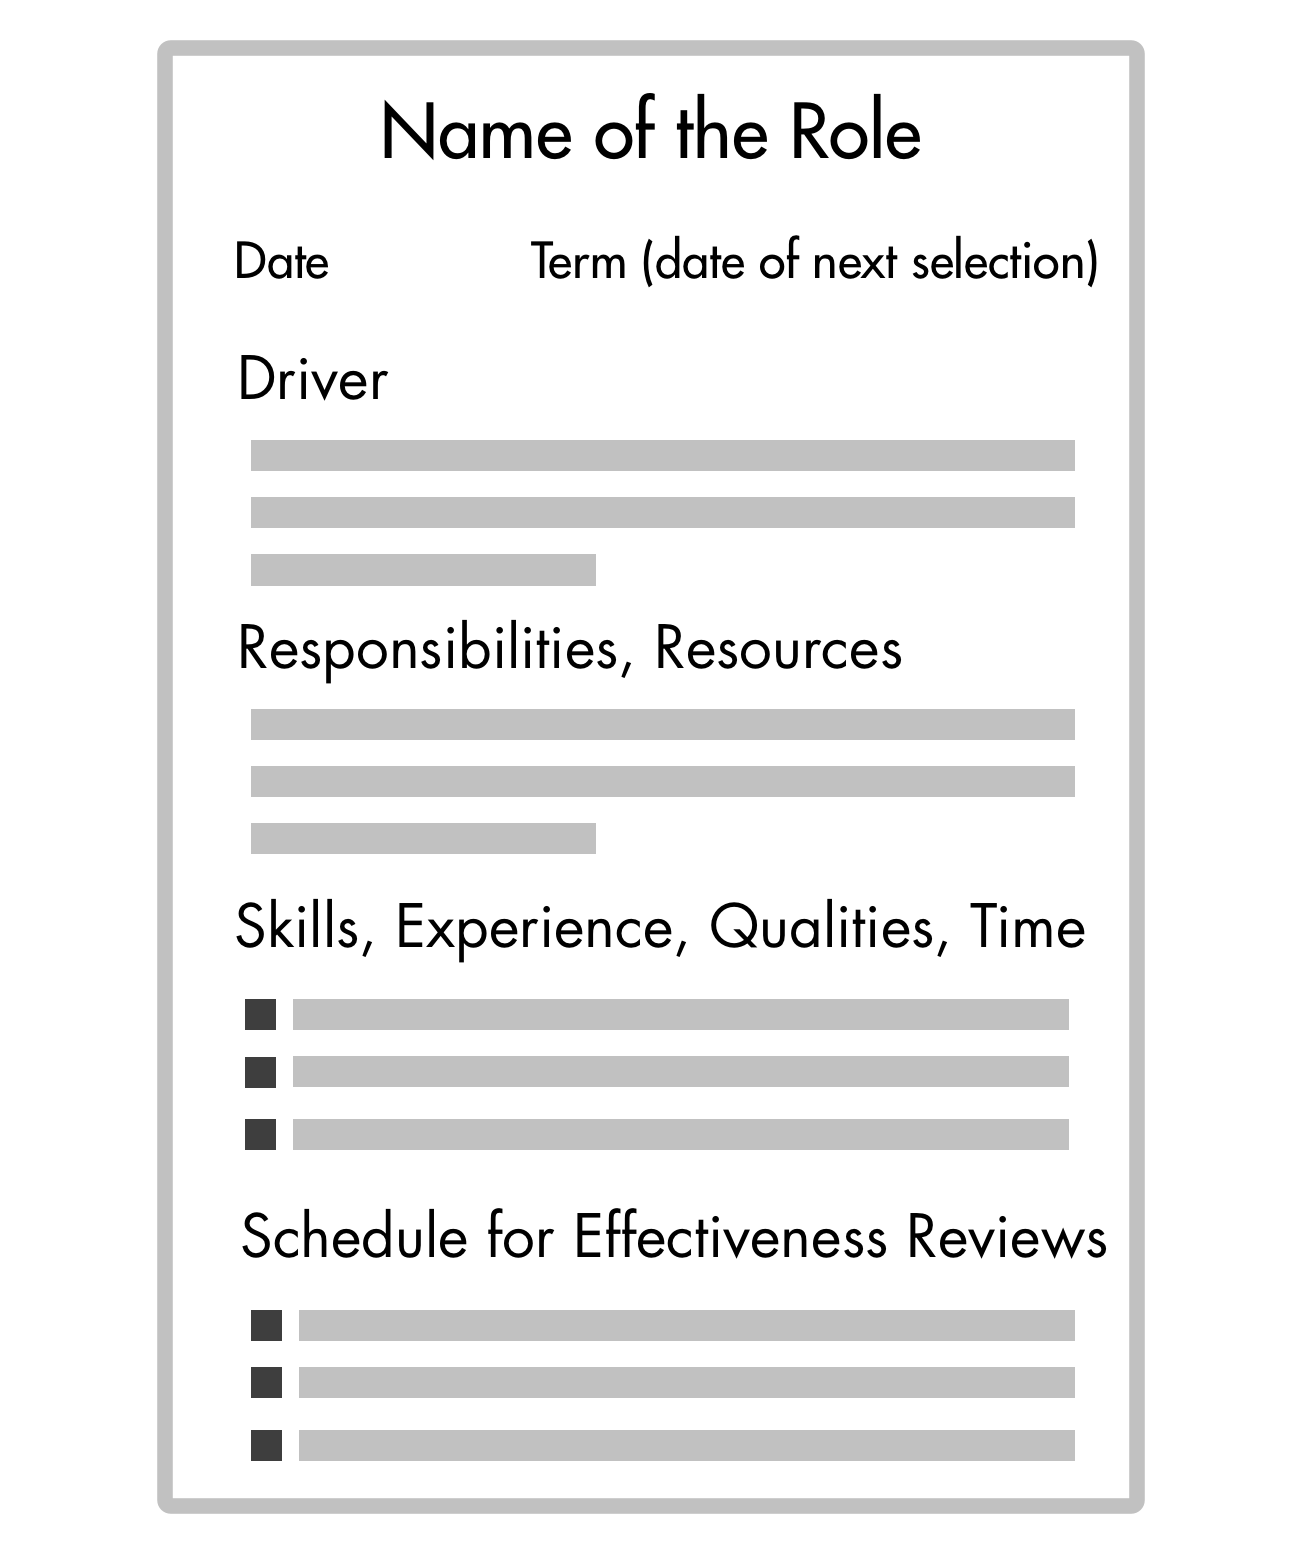
\includegraphics[keepaspectratio,width=\textwidth,height=0.75\textheight]{img/people-and-roles/role-description-template.png}
\end{figure}

\section{Role Selection}
\label{roleselection}

\begin{figure}[htbp]
\centering
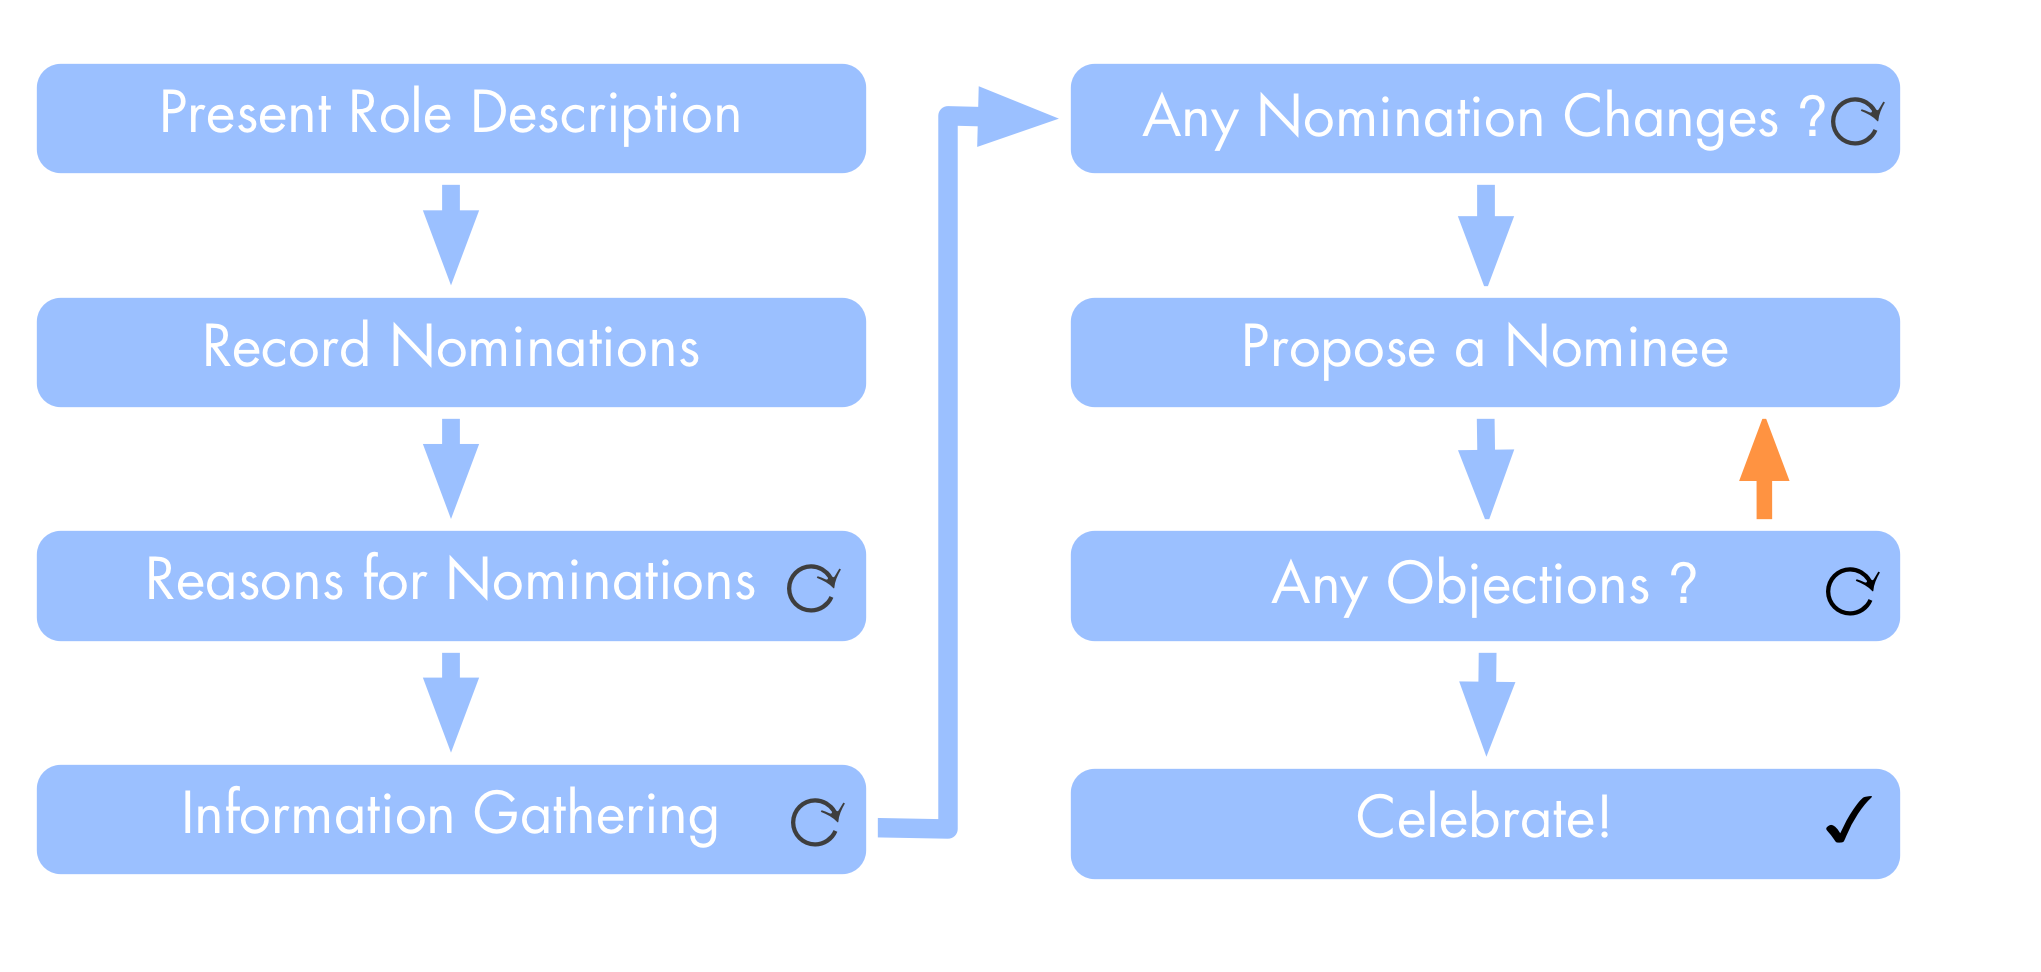
\includegraphics[keepaspectratio,width=\textwidth,height=0.75\textheight]{img/people-and-roles/selection.png}
\end{figure}

\begin{itemize}
\item People avoid expressing interest before elections

\item Nominations are made on the strength of the reason

\begin{itemize}
\item not according to the majority

\end{itemize}

\item You can nominate yourself or pass

\item When harvesting objections, ask the candidate last

\item Objections may be resolved by amending the role description or by nominating someone else

\end{itemize}

\section{Support Roles}
\label{supportroles}

{\ldots}

\chapter{Organizational Structure}
\label{organizationalstructure}

The primary function of organizational structure is \textbf{to enable effective collaboration} by aligning the flow of information to support the flow of value..

\textbf{Organizational structure needs to evolve continuously} in order to adapt to a changing environment.

\textbf{Semi-autonomous, self-organizing and self-governing circles} are the basic building blocks for organizational structure.

\section{Structural Patterns}
\label{structuralpatterns}

\begin{itemize}
\item Sociocracy 3.0 describes a variety of patterns to grow organizational structure

\item patterns apply to different layers of abstraction (basic, micro, macro and meta)

\item different patterns serve different drivers

\item patterns can be combined as needed

\item more patterns are out there and will be discovered

\end{itemize}

\section{Backbone Organization}
\label{backboneorganization}

A pattern for multi-stakeholder projects or services.

\begin{figure}[htbp]
\centering
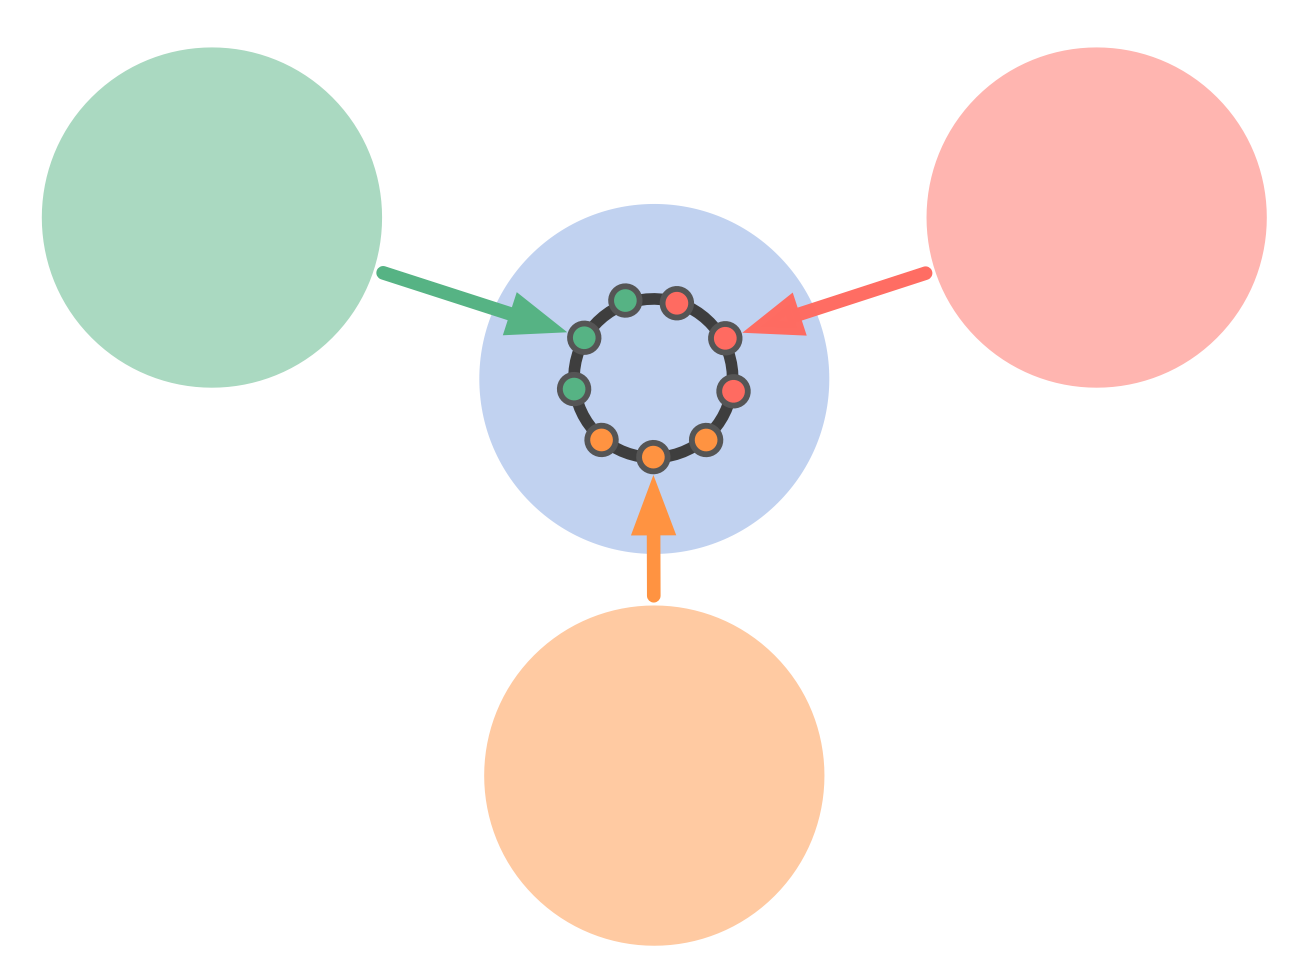
\includegraphics[keepaspectratio,width=\textwidth,height=0.75\textheight]{img/structural-patterns/backbone-organization.png}
\end{figure}

\section{Coordination Circle}
\label{coordinationcircle}

{\ldots}

\section{Delegate Circle}
\label{delegatecircle}

A pattern for coordination

\begin{figure}[htbp]
\centering
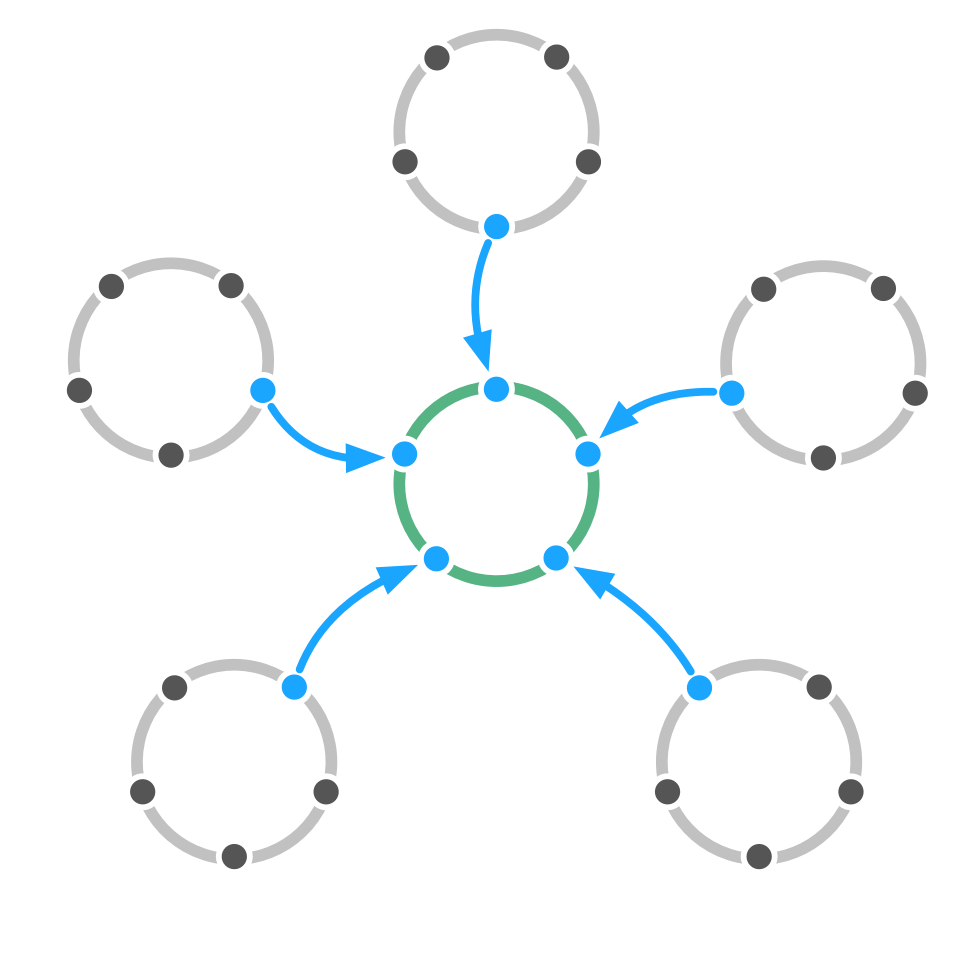
\includegraphics[keepaspectratio,width=\textwidth,height=0.75\textheight]{img/structural-patterns/delegate-circle.png}
\end{figure}

\section{Double Linking}
\label{doublelinking}

\begin{figure}[htbp]
\centering
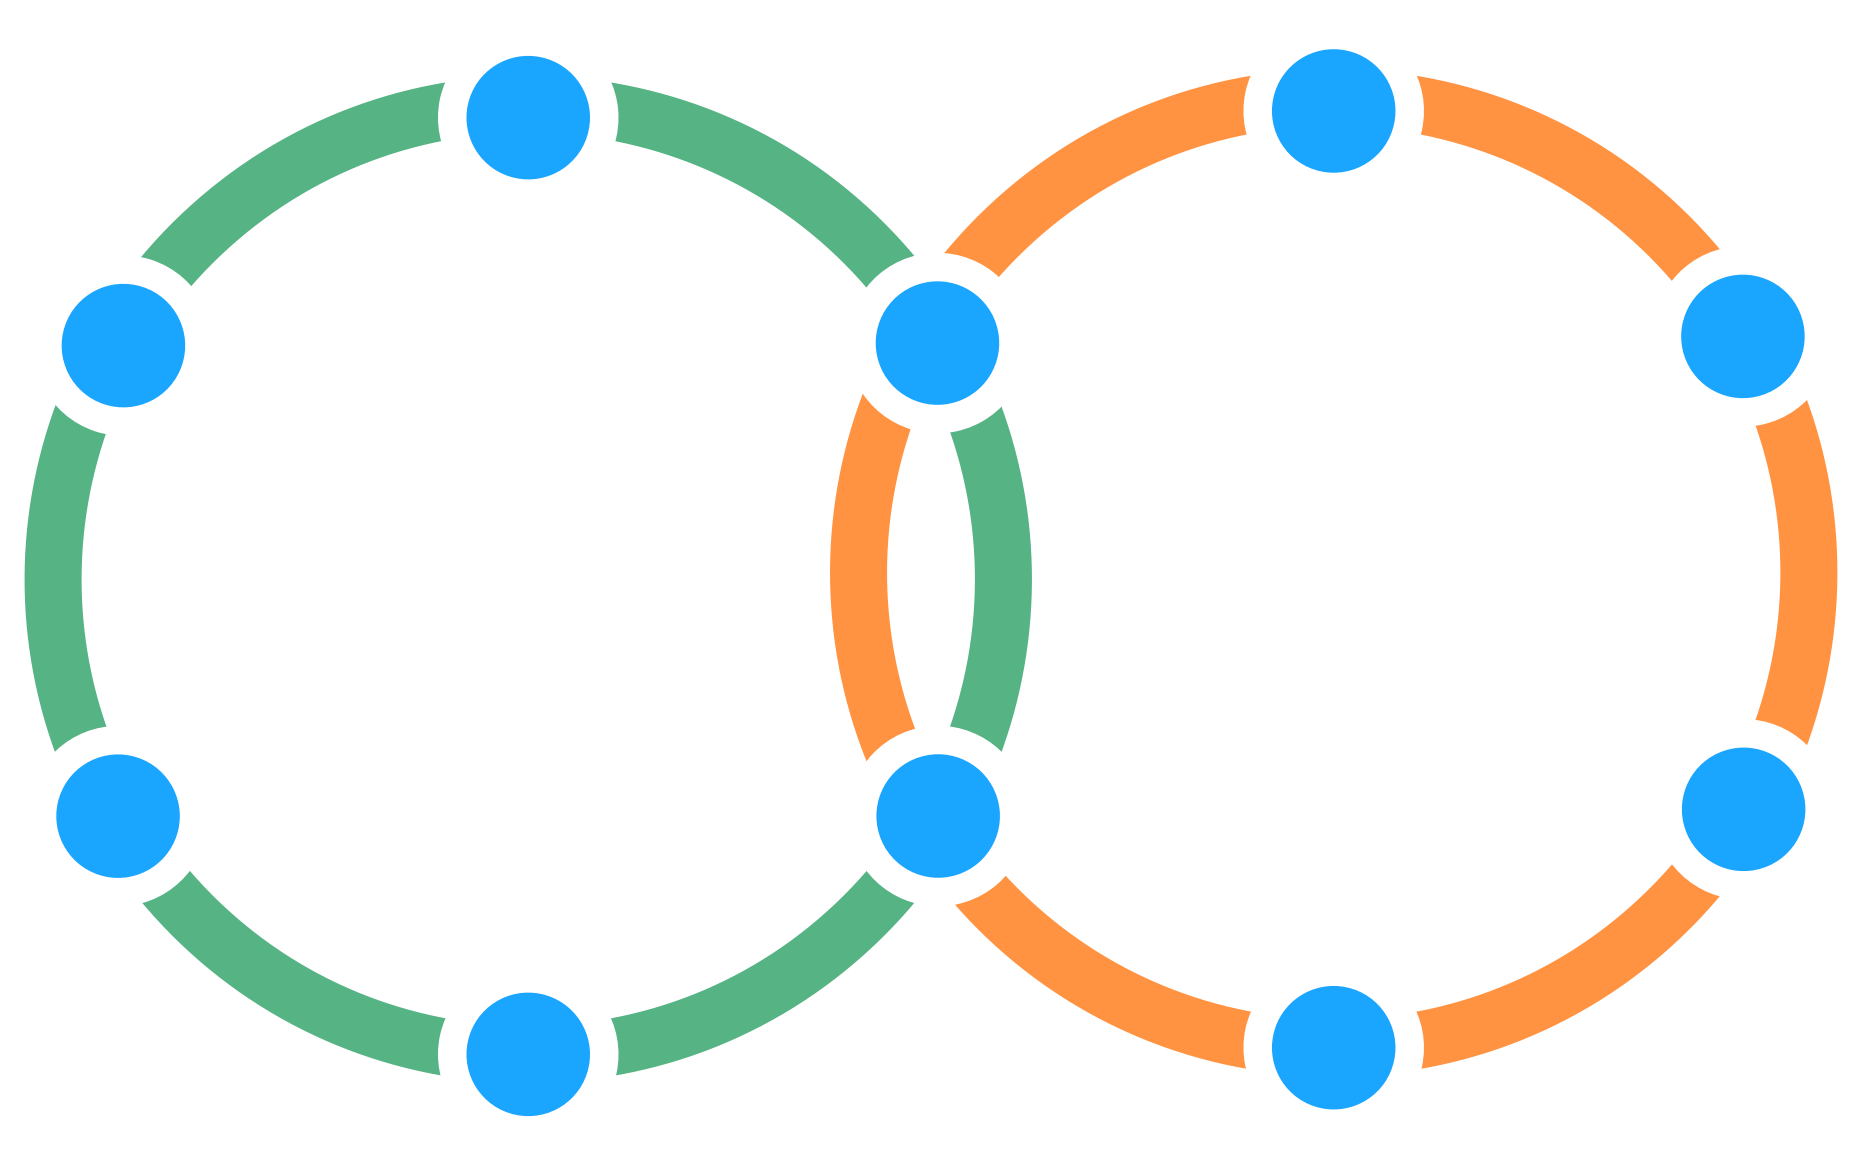
\includegraphics[keepaspectratio,width=\textwidth,height=0.75\textheight]{img/structural-patterns/double-link.png}
\end{figure}

\subsection{Facilitate two-way flow of information and influence}
\label{facilitatetwo-wayflowofinformationandinfluence}

\begin{itemize}
\item Two interdependent circles each elect a representative to participate as full members in both circles' governance meetings

\item can be used to prevent tensions in hierarchical structures

\end{itemize}

\section{Double-Linked Hierarchy}
\label{double-linkedhierarchy}

A pattern for the early phase of a transformation \#\#

\begin{figure}[htbp]
\centering
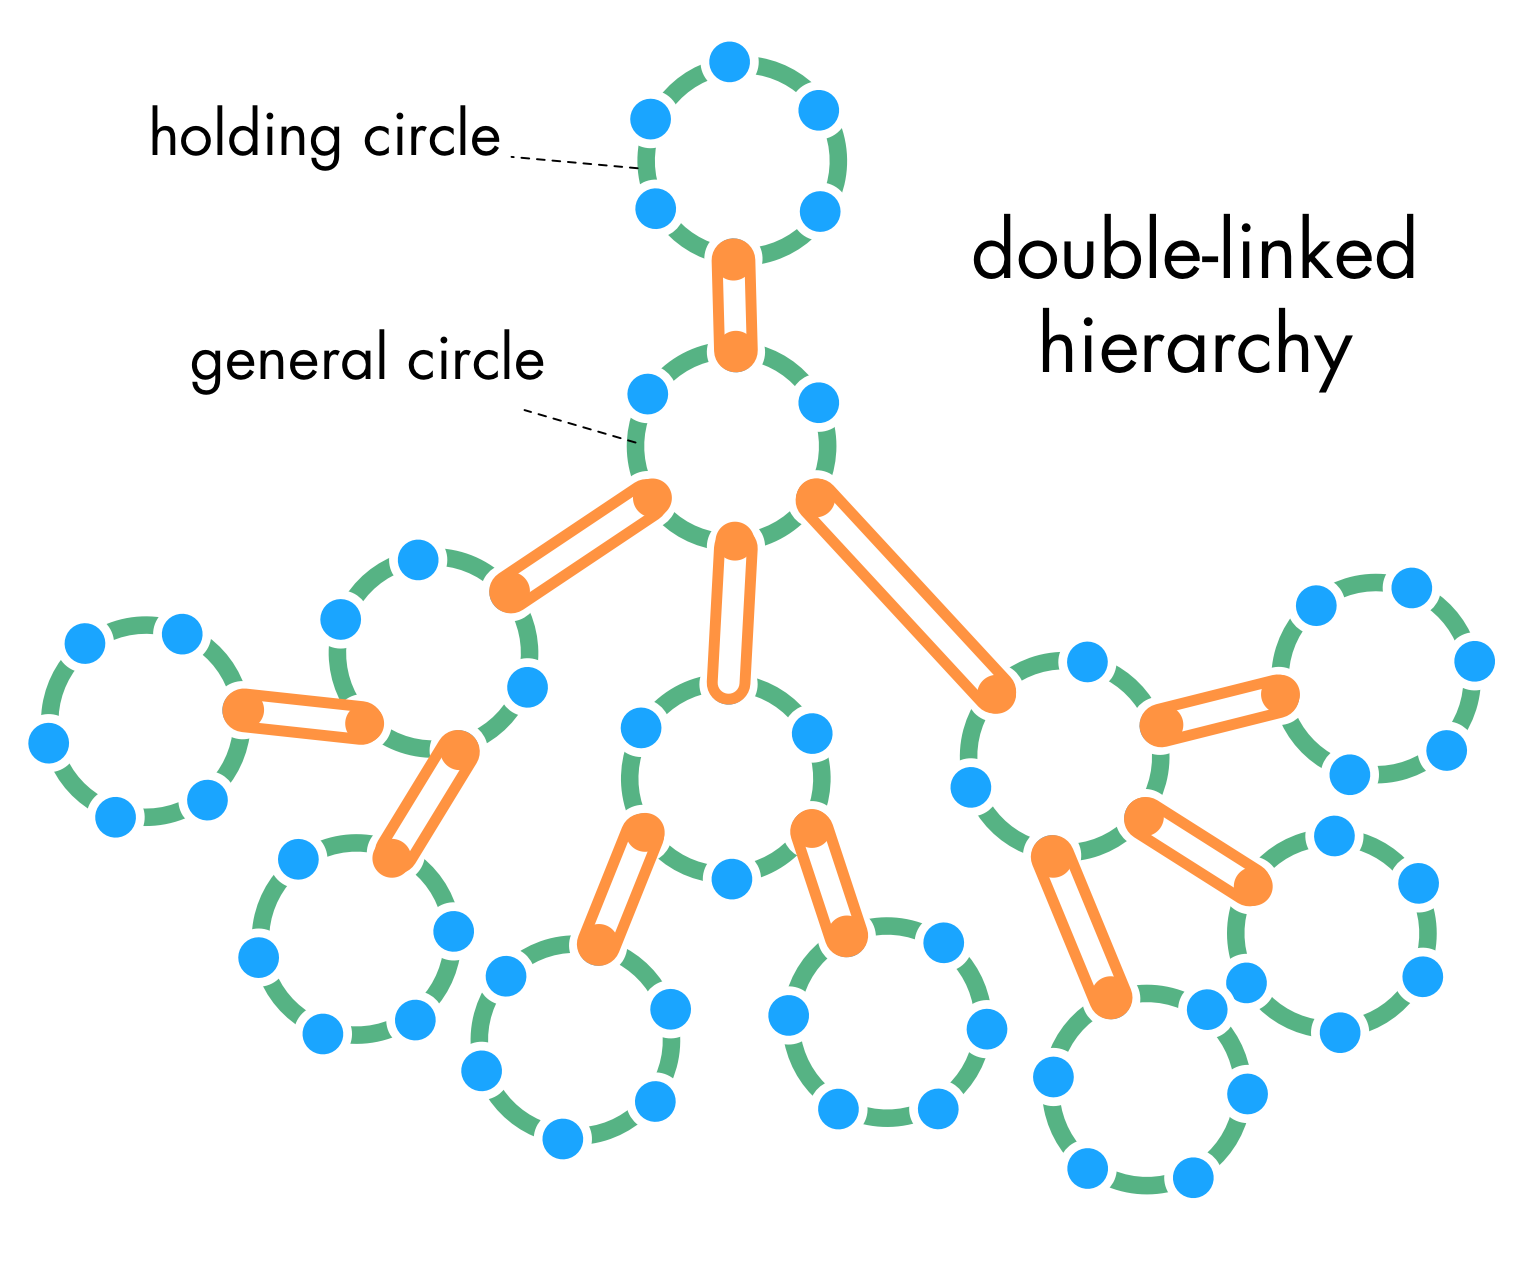
\includegraphics[keepaspectratio,width=\textwidth,height=0.75\textheight]{img/structural-patterns/double-linked-hierarchy.png}
\end{figure}

\section{Fractal Organization}
\label{fractalorganization}

A Pattern for learning, coordination and alignment across organizational boundaries.

\begin{figure}[htbp]
\centering
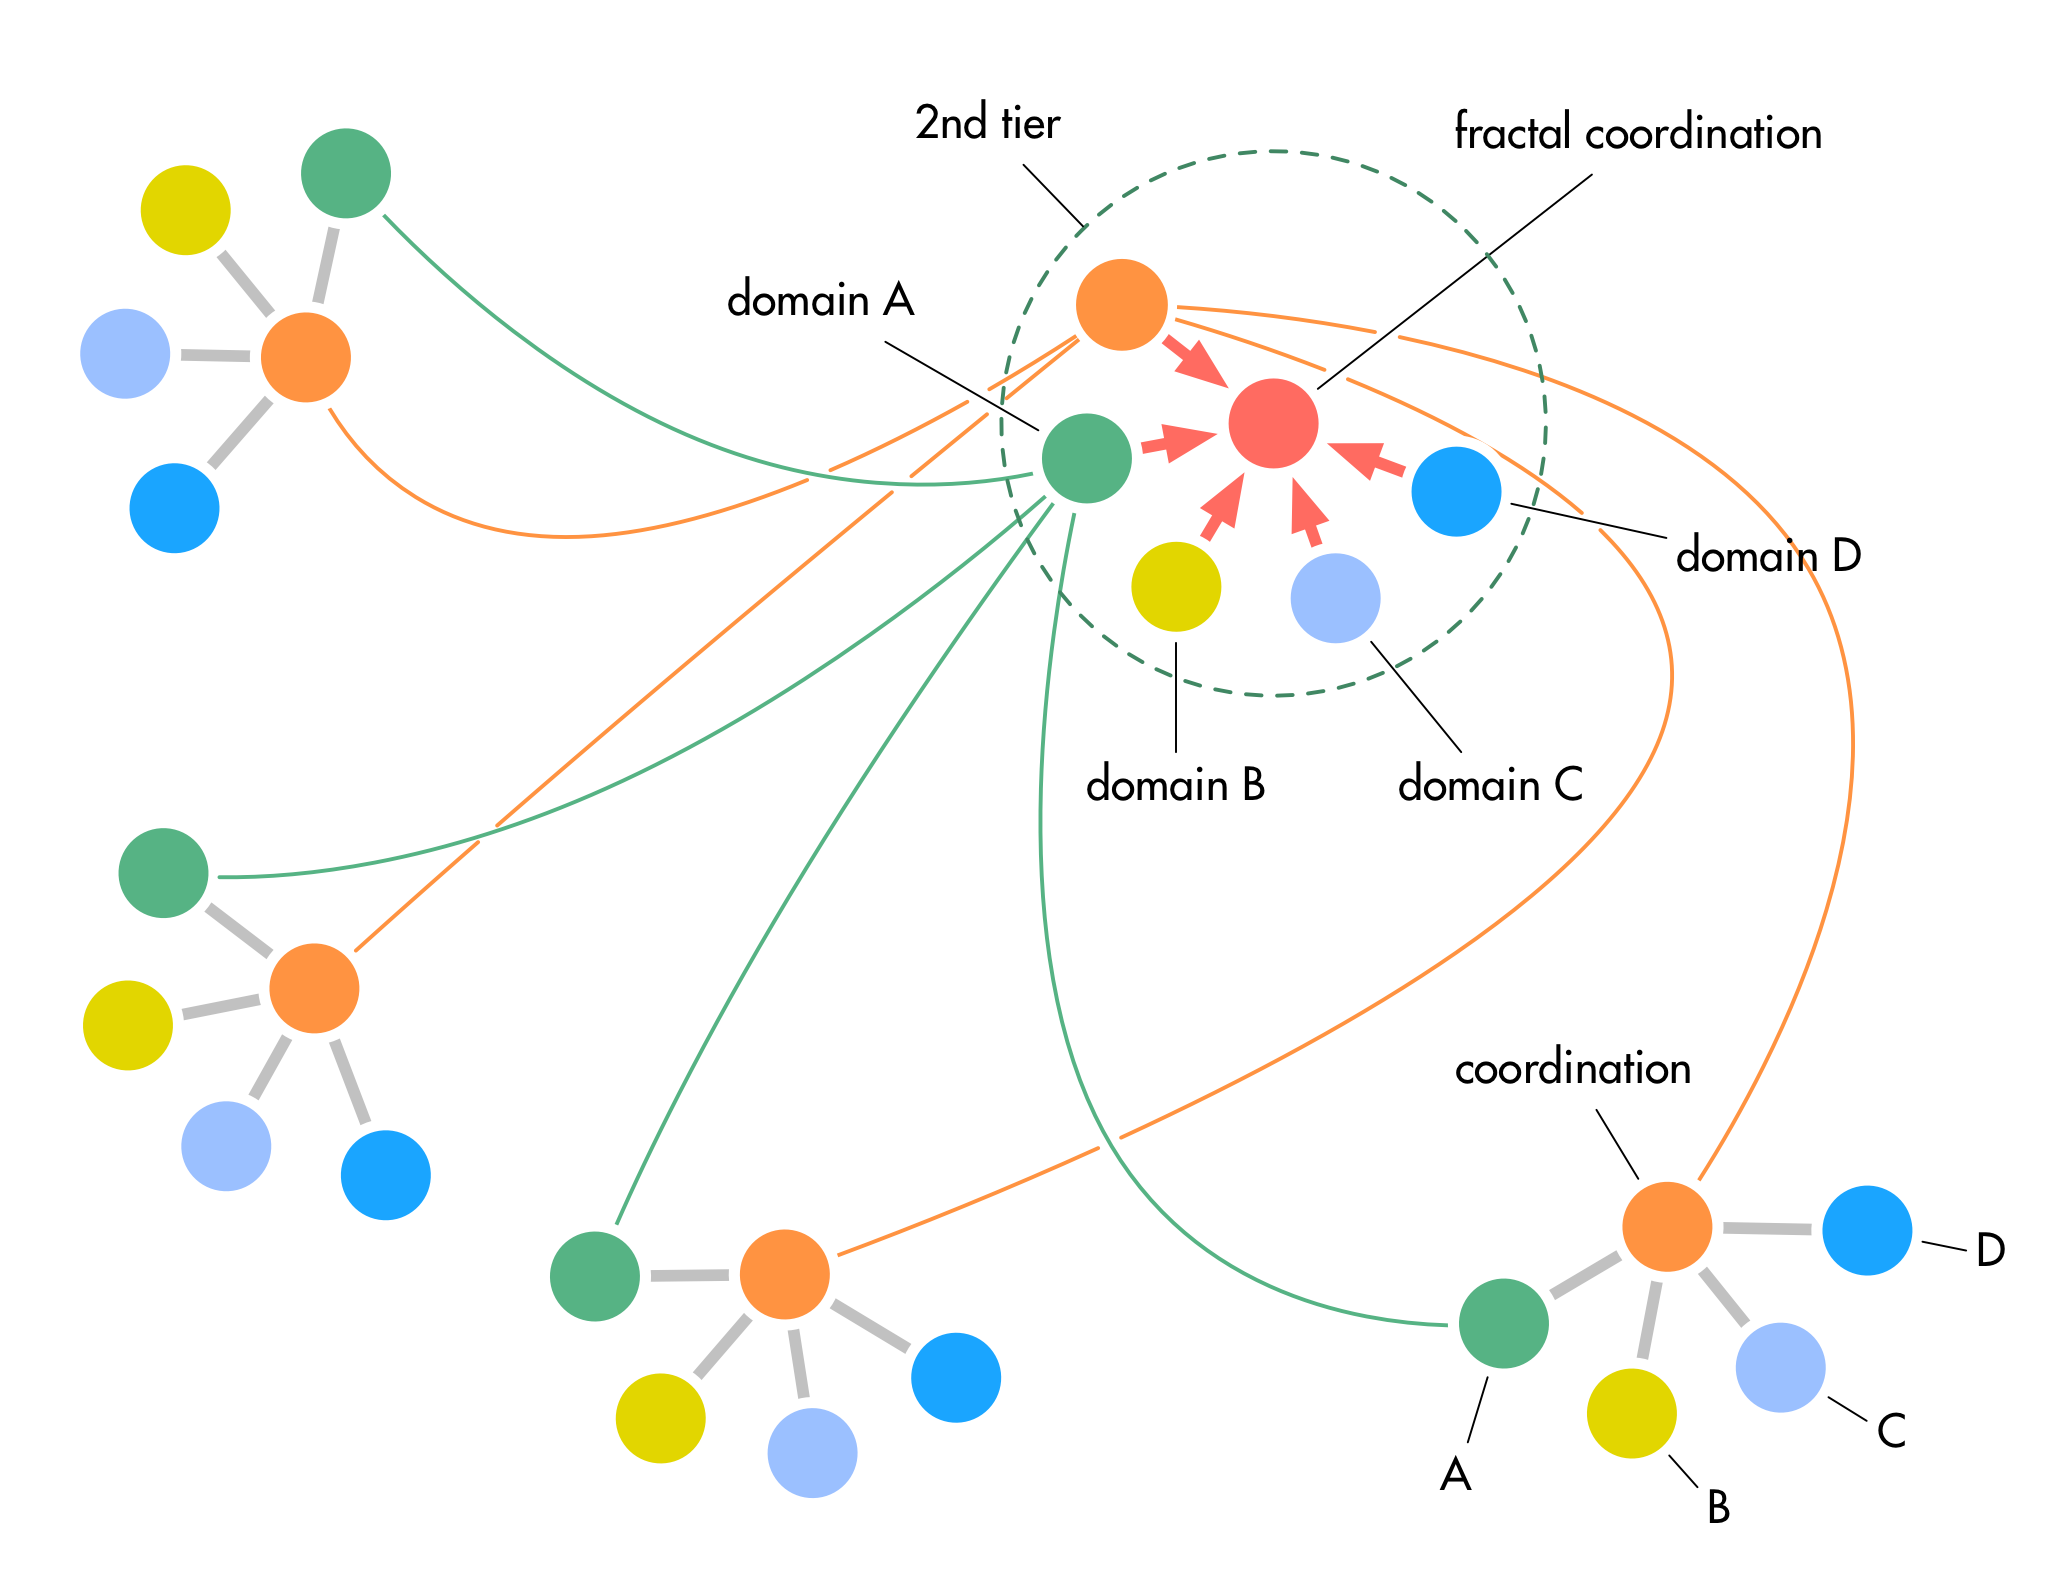
\includegraphics[keepaspectratio,width=\textwidth,height=0.75\textheight]{img/structural-patterns/fractal-organization.png}
\end{figure}

\section{Helping Circle}
\label{helpingcircle}

\textbf{Driver}

\begin{itemize}
\item a circle requires a simple service, but has not enough capacity

\end{itemize}

A group of people with the mandate to execute on rules and guidelines set by the circle that encloses or ``owns'' the helping circle.

Within the boundaries defined by the rules and guidelines the helping circle might self-organize, or work with a coordinator or leader. A helping circle usually has no navigation meeting, but may raise objections to rules and guidelines to the parent circle.

\section{Nested Circle}
\label{nestedcircle}

A pattern for expanding functions

\begin{figure}[htbp]
\centering
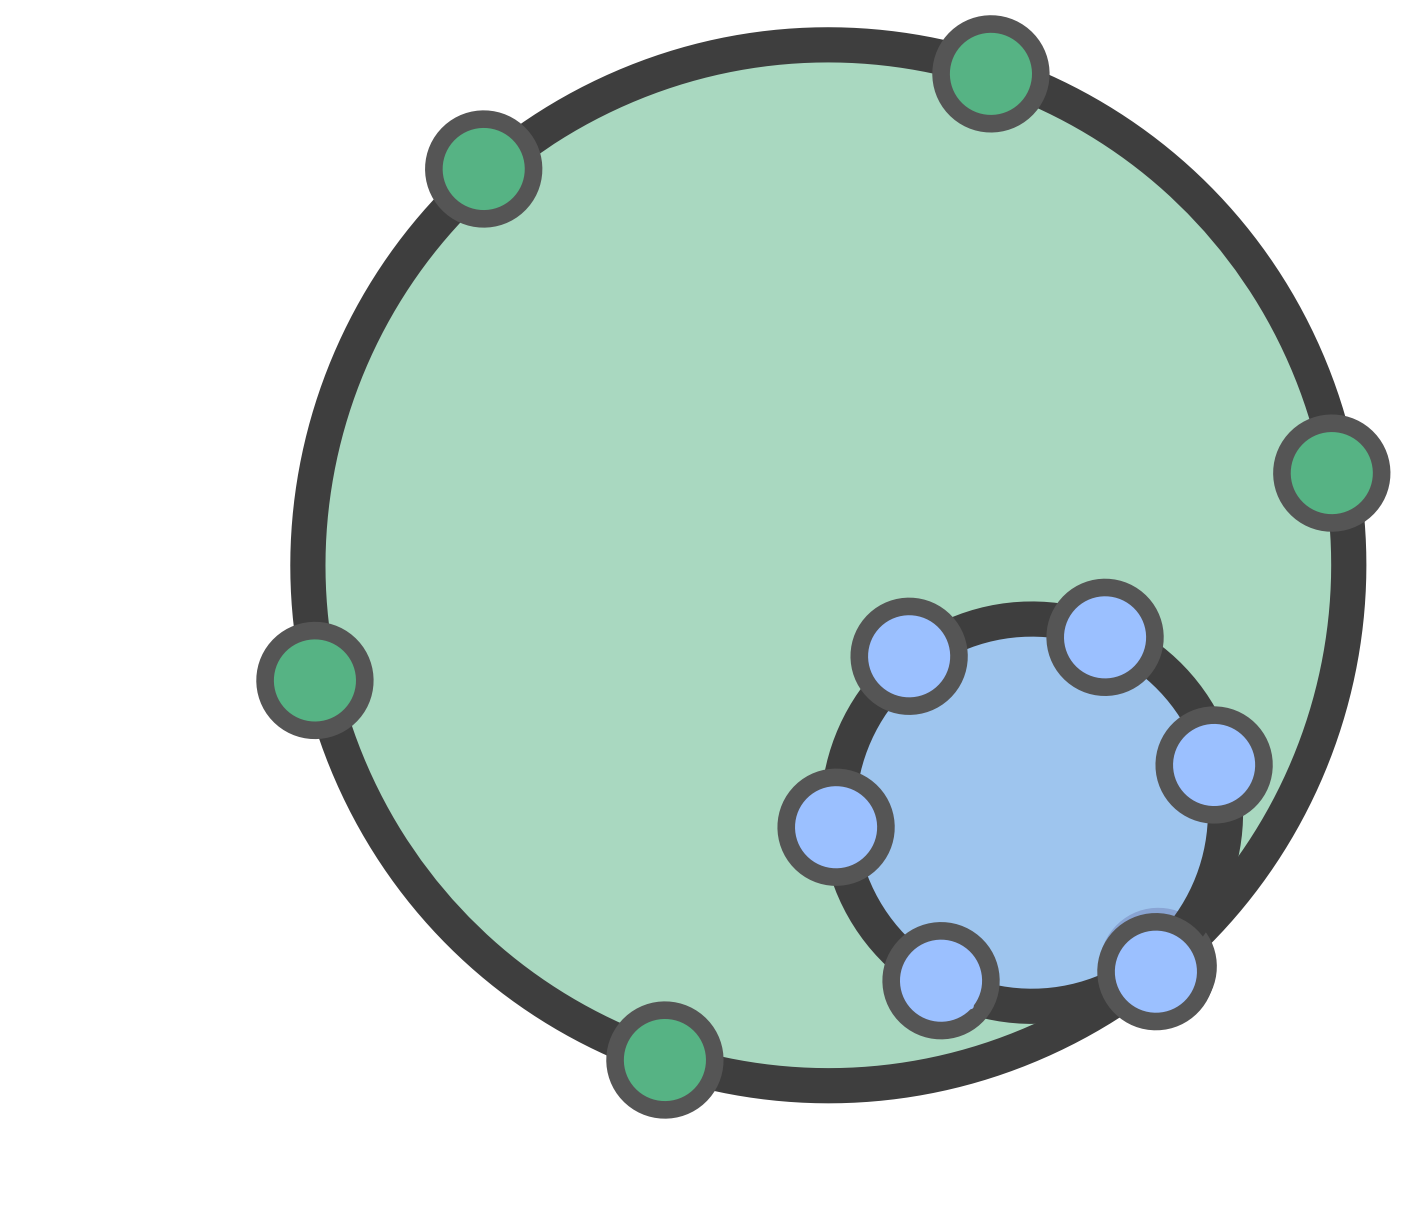
\includegraphics[keepaspectratio,width=\textwidth,height=0.75\textheight]{img/structural-patterns/nested-circle.png}
\end{figure}

\section{Peach Organization}
\label{peachorganization}

Periphery drives the organization, the center provides services.

\begin{figure}[htbp]
\centering
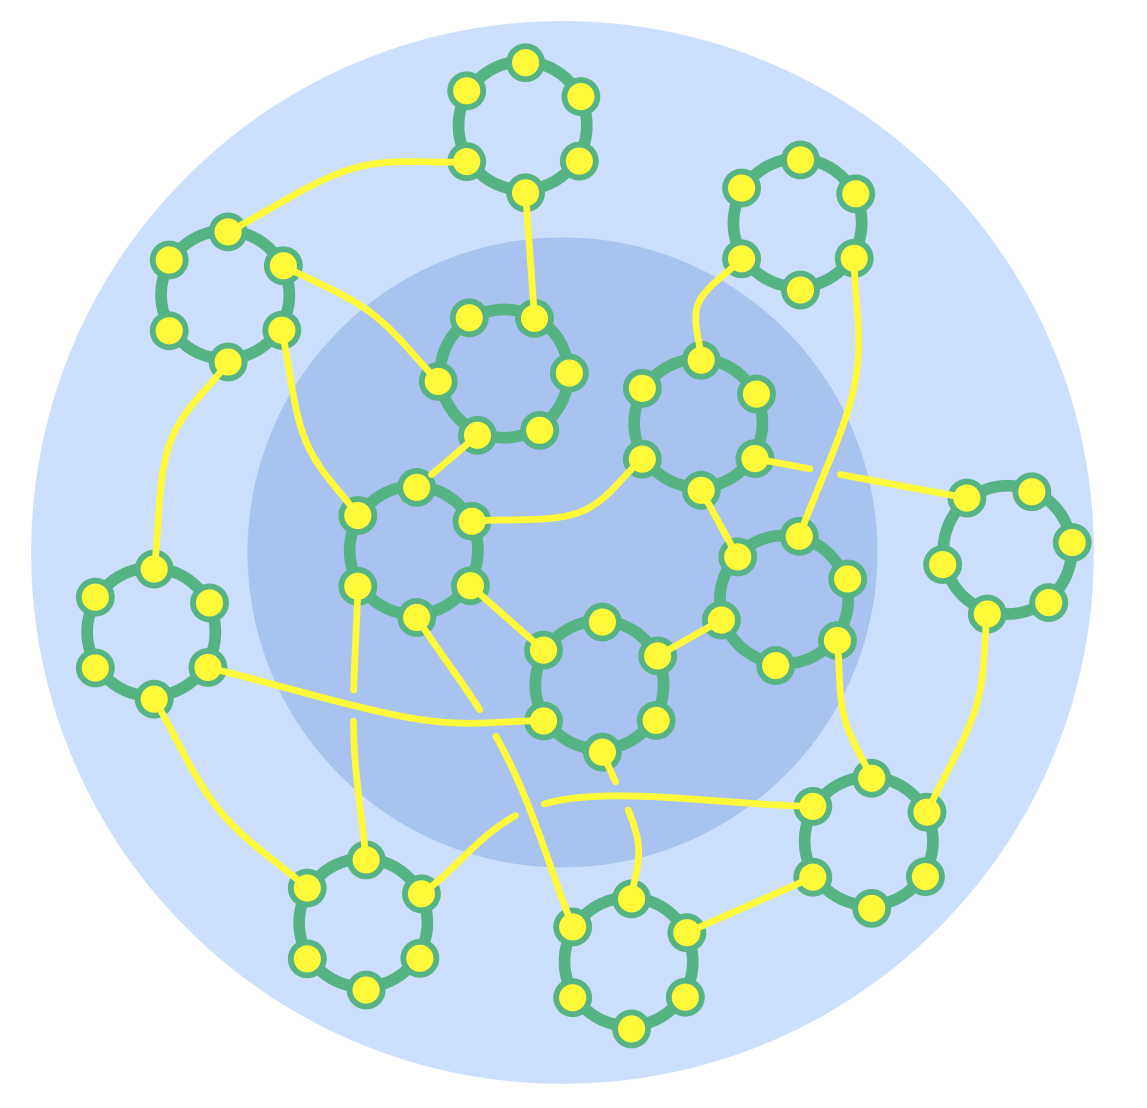
\includegraphics[keepaspectratio,width=\textwidth,height=0.75\textheight]{img/structural-patterns/peach-organization.png}
\end{figure}

\section{Representative}
\label{representative}

Representatives (a.k.a Links){\ldots}:

\begin{itemize}
\item {\ldots}stand for the interests of one circle in another circle

\item {\ldots}are elected for a limited term

\item {\ldots}participate as full members in governance meetings of the other circle and can:

\begin{itemize}
\item raise items for the agenda

\item object to agreements and proposals

\end{itemize}

\end{itemize}

\section{Service Circle}
\label{servicecircle}

A pattern for outsourcing shared services

\begin{figure}[htbp]
\centering
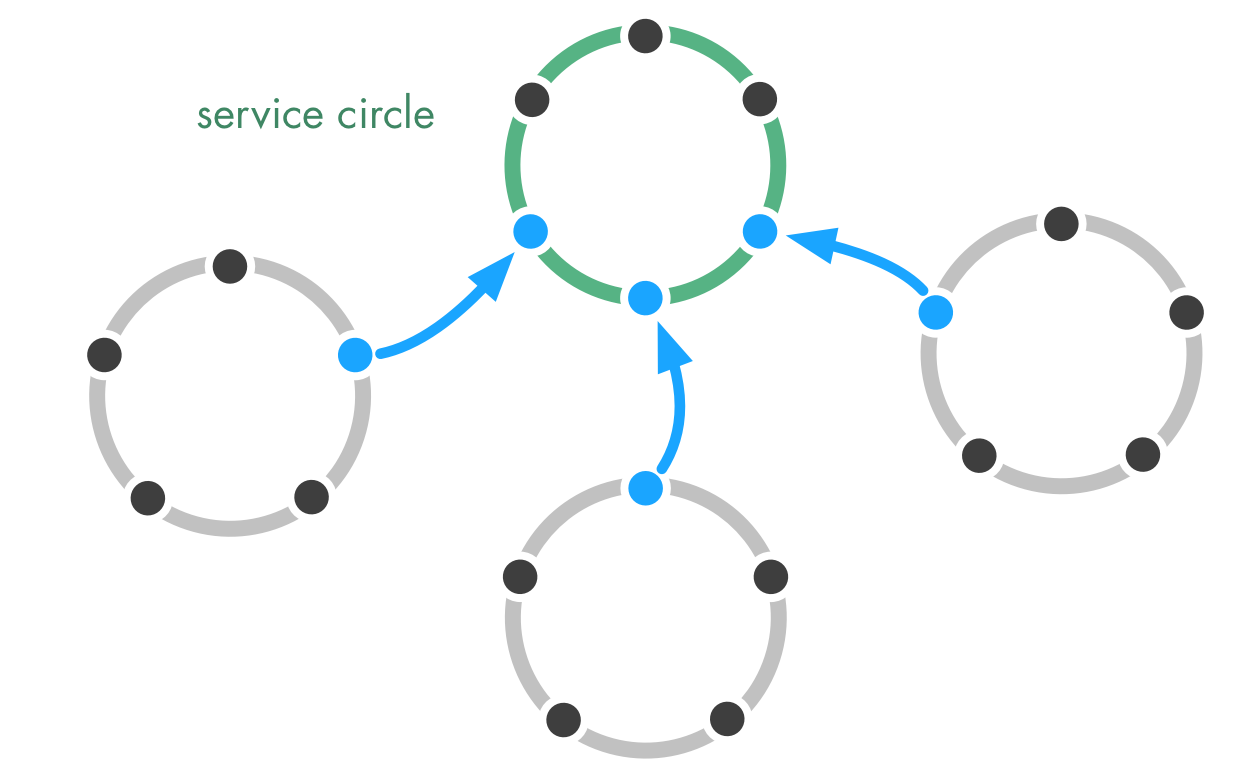
\includegraphics[keepaspectratio,width=\textwidth,height=0.75\textheight]{img/structural-patterns/service-circle.png}
\end{figure}

\chapter{Bringing In S3 Patterns}
\label{bringingins3patterns}

The patterns for introducing an organization to S3 are all based on the paradigm of inviting change.

\section{Adapt Patterns To Context}
\label{adaptpatternstocontext}

Patterns are merely ideas that worked for somebody somewhere, in their culture, their perception of the world, their strengths and growing edges. Your context is certainly different, so if you simply copy and paste a pattern, it might not work for you. This is why you sometimes need to adapt a pattern to your context.

\subsection{Context for Successful Application:}
\label{contextforsuccessfulapplication:}

In order to successfully adapt a pattern, a circle needs to develop shared understanding of both the pattern and their specific context. In almost every case it makes sense to gather the circle for this, to ensure both buy-in of all circle members and availability of all the knowledge and experience present in the circle. Often it's a good idea for everyone to review the pattern before the workshop.

\subsection{Application}
\label{application}

The basic steps of the process of adapting a pattern are very simple, and can be implemented in various levels of detail:

\begin{itemize}
\item develop shared understanding of the pattern and your context

\item co-create an adaptation of the pattern

\item evaluate effectiveness and evolve your adaptation

\item share your experience with others, and consider feeding back successful adaptations to the S3 handbook

\end{itemize}

\subsubsection{Understand the Pattern and Your Context}
\label{understandthepatternandyourcontext}

Here's a set of activities to guide you, pick those you find valuable for you. It's up to the facilitator to facilitate them in rounds or as a brainstorming, and to visualize all the results in a way they can be seen by all participants. Give space for questions, so at the end everyone feels they understand the outcome.

\begin{itemize}
\item What is the \textbf{problem the pattern aims to solve}? How does this match to your driver for seeking out this pattern? Note similarities and differences.

\item What is the \textbf{context for successful application} of the pattern? List both the common ground and the differences to your context?

\item If the pattern describes \textbf{variants}, determine which variant might be the best fit for you. It is this variant you would attempt to adapt first.

\item Does your context match one or several of the \textbf{known limitations} or disadvantages of a pattern? Make a note which ones.

\item If the pattern description lists \textbf{advantages}, mark the ones you would want to preserve.

\item If the patterns contains \textbf{references} to other patterns, go and see if they contain something to help you.

\item How does the pattern relate to each of the \textbf{seven principles behind S3}? Note what is important and should be preserved.

\end{itemize}

\subsubsection{Co-Create an Adaptation of the Pattern}
\label{co-createanadaptationofthepattern}

A simple an effective way for creating an adaptation of a pattern is \href{proposal-forming.md}{Proposal Forming}\footnote{\href{proposal-forming.md}{proposal-forming.md}}, where you can use the output of the first phase as considerations or ingredients for your adaptation.

Considering \href{intended-outcome.md}{Intended Outcome}\footnote{\href{intended-outcome.md}{intended-outcome.md}} and \href{evaluation-criteria.md}{Evaluation Criteria}\footnote{\href{evaluation-criteria.md}{evaluation-criteria.md}} of your proposed adaptation will help you evaluate and evolve the patterns later.

The proposal needs to be agreed upon by the circle, e.g. by using \href{consent-decision-making.md}{Consent Decision Making}\footnote{\href{consent-decision-making.md}{consent-decision-making.md}}

\subsection{Variants}
\label{variants}

If you feel that everyone has a solid understanding of the context and the pattern anyway, e.g. because you are already using it for a while and experience limitations, you might skip the first part and go right into \emph{Proposal Forming}.

A circle might also appoint one or several members to create a proposal for an adaptation in any way they see fit, e.g. by using the activities for understanding pattern and context suggested above, and then present the proposal to the circle, e.g. in the \href{navigation-meeting.md}{Navigation Meeting}\footnote{\href{navigation-meeting.md}{navigation-meeting.md}}.

\subsection{Known Limitations}
\label{knownlimitations}

Adapting patterns works best when everyone involved is invested in understanding S3 principles, the pattern in question and the context of the circle. Some circles have a culture of high resistance to things they did not develop themselves, or they have pain points or blind spots which make it difficult to approach some patterns with an open mind.

\section{Be The Change}
\label{bethechange}

Be the change you want to create, tell the story how you discovered S3. Invite others for experiments, invite them to share their stories, learn and grow together.

\section{Continuous Improvement Of Work Process}
\label{continuousimprovementofworkprocess}

{\ldots}

\section{Open S3 Adoption}
\label{opens3adoption}

Instead of mandating S3, the formal authorities make the call for members of the organization to get together in an Open Space and invite them to co-create experiments they'd like to conduct around S3 patterns. This usually happens after some small experiments in an organization demonstrated the potential of S3.

Conducting the first Open Space:

\begin{itemize}
\item explain boundaries for experiments: S3 principles and patterns

\item explain Open Space rules and principle

\item co-create agenda

\item provide space to share experiences and ideas between sessions

\item provide a platform for announcing initiatives and experiments

\item announce next Open Space

\end{itemize}

In regular intervals, usually twice a year, the whole organization will get together again in an Open Spaces to evaluate experiment and design new ones. In between Open Spaces formal authorities support the experiments and collect stories.

This pattern is based on OpenSpace agility (formerly Open Agile Adoption) by Dan Mezick.

\section{Pull-System For Organizational Change}
\label{pull-systemfororganizationalchange}

Change in organization (e.g. reorganizations), is commonly designed by a small group of people, often without even consulting many those affected by that change. This is not only a sure way of creating resistance to change in people, it also does not take into account the actual capacity for change, often overloading the system and therefore reducing the overall capacity of the system - the exact opposite of the intended outcome of the change. This often leads to the even more change in search of increased effectiveness.

When instead of mandating change, we create a pull-system for change by giving the people decision making power over all agreements which affect them, they will be able to navigate both scope and speed of organizational changes themselves, growing a learning organization with a much greater chance of recovering from overload and usually preventing it altogether.

Over time, this will allow for the transition from organizational change as a mere reaction to changes in the environment (e.g. the market) towards intentional change.

In context to S3, organizational change is creating and evolving agreements about how we organize and collaborate, sometimes in the form of agreeing to experiment with new patterns from S3.

S3 contains various patterns which are helpful for empowering people to pull in organizational change, here's a shortlist of where to look first:

\begin{itemize}
\item At the very beginning, you need to invite people to learn more about S3, e.g. through the pattern \emph{Be The Change}

\item when the group understands and \emph{Adopts S3 Principles}, the principles can serve as an anchor for discussing potential solutions

\item \emph{Consent Decision Making} helps people to make decisions without becoming overwhelmed

\item even if you don't go for decisions by consent right away, e.g. because you operate in a low trust environment, \emph{Proposal Forming} can be used to tap creativity and wisdom of the group when preparing organizational change

\item developing shared understanding of \emph{Drivers} enables groups to find more effective solutions to problems

\item \emph{Navigate via Tensions} helps identify and tackle the most relevant challenges

\end{itemize}

Of course, taking responsibility for all decisions that affect them is tough to swallow for many groups, and different members will have a different understanding of what makes a good decision making process. To reduce resistance, simply invite the group to try \emph{Proposal Forming} and \emph{Consent Decision Making}as an experiment for a month. In the absence of objections, schedule a review session with everyone one month in the future. This will create a safe space for each participant to develop an understanding of their contribution in this new way of making decisions a being accountable. They will learn to trust in the circle to make decisions every can live with, and to bring about change in a pace the circle can sustain. Depending on an organization's culture or a circle's history, mentoring and coaching is helpful to support the circle in moving out of their comfort zone and discovering their true capacity for change.

\chapter{Alignment}
\label{alignment}

The patterns in this section help an organization align on many different levels.

Adopt S3 Principles and Agree on Values help establish general guidelines we can all agree on, and thus reduce the number of explicit agreements we need to make, Contracting and Accountability brings clarity around the relationship of the individual to the organization, Transparent Salary offers a perspective of aligning agreements on compensation with the principles of S3.

\section{Adopt S3 Principles}
\label{adopts3principles}

\textbf{Driver}:

\begin{itemize}
\item principles are reflected in all patterns

\item chosen values (or implicit assumption) guide behavoiur

\item need: align chosen values and S3 principles to reduce tension with S3 patterns

\item need: understand principles for correct application of patterns

\end{itemize}

All patterns contained in S3 are built on seven core principles: consent, empiricism, equivalence, accountability, effectiveness, transparency and continuous improvement.

\begin{figure}[htbp]
\centering
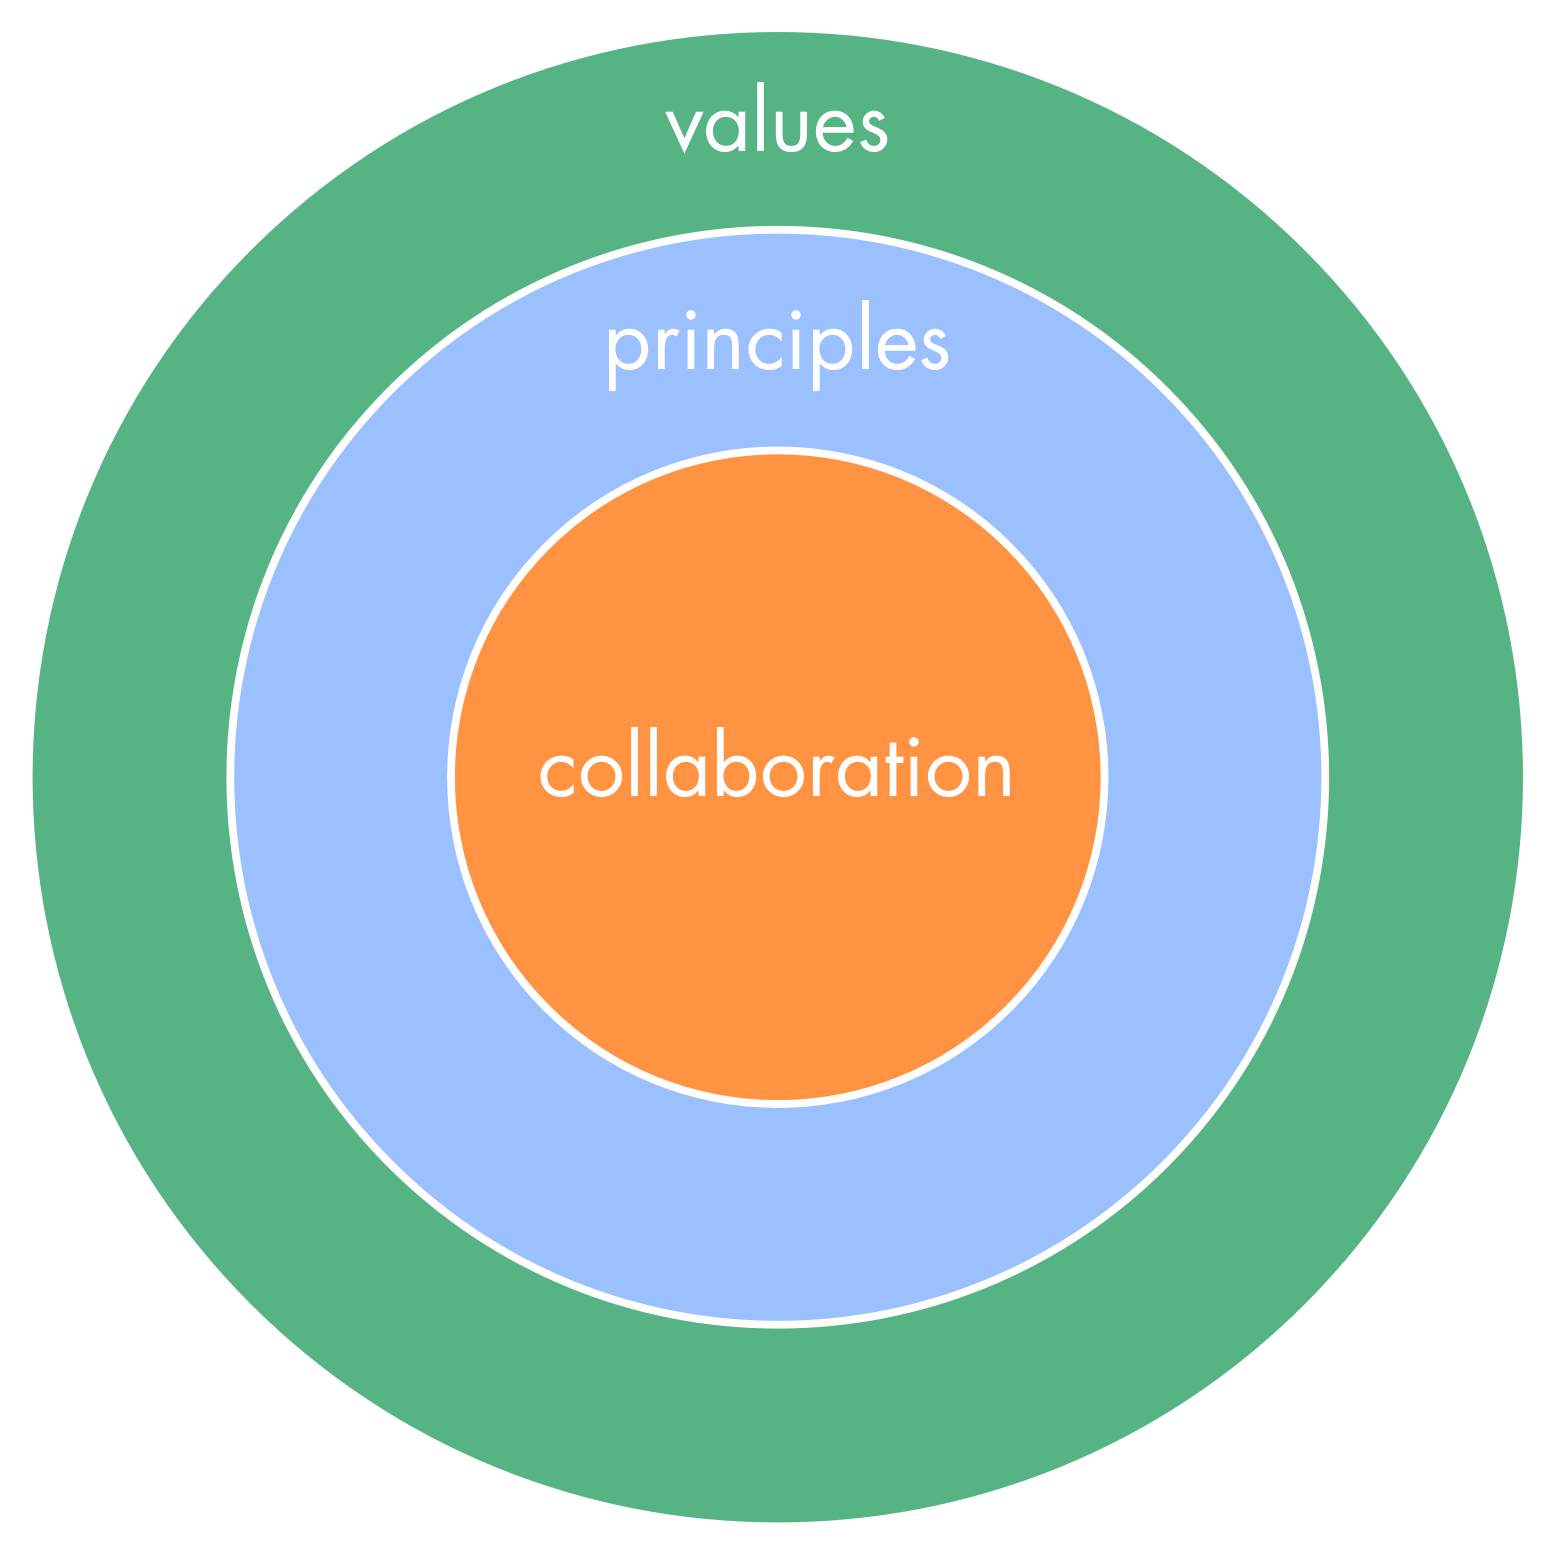
\includegraphics[keepaspectratio,width=\textwidth,height=0.75\textheight]{img/collaboration-values/values-step3.png}
\end{figure}

When we \textbf{Agree On Values}, we need to check how our chosen values relate to S3's principles, if there's a conflict, this will most likely result tensions with at least some of S3's patterns .

Our chosen values should be unique for our organization, they're how we define our specific culture.

However, we can also agree on adopting S3's principles as an additional set of general principles to guide our actions and interactions.

This agreement would include three different aspects:

\begin{itemize}
\item how can we make sure everyone knows and unserstands the 7 principles?

\item what can we do to help each other apply the 7 principles?

\item what do we do when we suspect one or more principles are violated in a certain situation?

\end{itemize}

Each organization or group needs to find their own answers for these questions, e.g. through \emph{Proposal Forming}, here's a few examples:

\begin{itemize}
\item learn and understand: print the descriptions of the principles form this handbook for everyone, then get together, pick a pattern from the handbook (at the beginning stick to those you already use), and discuss how this pattern relates to each of the principles

\item support each other in application: have a poster with the agreements in your meeting room, so when making an agreements, you are reminded to check how a proposal relates to each of the principles

\item suspected conflict with principles: agree on a protocol for raising concerns or asking about the intended outcome of a proposal or somebody's actions in relation to the 7 principles.

\end{itemize}

\section{Agree On Values}
\label{agreeonvalues}

A pattern for setting boundaries for behavior, decisions and actions by adopting a set of values that is shared throughout an organization.

\textbf{Motivation for this pattern:} Culture in an organization is formed through implicit assumptions or explicit agreements about acceptable behavior. Agreements and assumptions can vary throughout an organization.

Making an explicit commitment to aligning behavior, decisions and actions along shared values improves effectiveness. A \textbf{value} is a principle of some significance that guides behavior. \textbf{Chosen values} are an intentional and collaborative effort to create the culture people want to see in an organization.

\subsection{Indicators for using this pattern}
\label{indicatorsforusingthispattern}

\subsubsection{Conditions:}
\label{conditions:}

\begin{itemize}
\item lack of shared understanding of the ethical boundaries of decisions and actions across an organization

\item more or less radically different cultures in different parts of an organization

\item culture in an organization appears to impede greater effectiveness

\end{itemize}

\subsubsection{Needs:}
\label{needs:}

\begin{itemize}
\item bring members of an organization closer together and align teams

\item develop norms that compliment objectives

\item reduce investment required for making effective decisions

\end{itemize}

\subsection{The details}
\label{thedetails}

When discussing shared values, it can be challenging for the members of an organization to identify and articulate their shared intrinsic values, because their personal values meet with \textbf{explicit and implicit assumptions about expected and appropriate behavior} in the organization. Additionally these assumptions may depend on context, e.g. people behave differently when a CEO is present in a meeting, and there's often different cultures in different parts of the organizations, e.g. in engineering, sales and management.

Therefore it's usually easier for people to focus on what behavior they consider as supportive of effective collaboration.

These are their \textbf{chosen values} - the set of values members agree on and commit to in an intentional and collaborative effort of aligning towards both achieving organizational objectives and growing the kind of culture they want to see.

Chosen values support effectiveness of an organization by:

\begin{itemize}
\item offering \textbf{guidance} to determine appropriate action or behavior, often reducing the need for more specific agreements.

\item reducing potential for \textbf{misunderstanding}

\item \textbf{aligning} decision making and action

\item \textbf{inviting contribution} of all its members

\item \textbf{attracting new members, partners and customers} in natural alignment with the organization

\end{itemize}

\subsubsection{Putting it into practice}
\label{puttingitintopractice}

Since commitment to a set of chosen values is an experiment, an organization benefits from developing strategies for:

\begin{itemize}
\item supporting each other in developing shared understanding of the values and for applying them consistently

\item learning when values might be updated, refined, or even dropped

\item responding to situations where individuals suspect a value may have been compromised or overlooked

\item discovering and changing existing practices or agreements that stand in the way of adopting a shared value

\end{itemize}

As an organization grows structure it is natural that different flavors of culture evolve in different domains. Alignment with chosen values across an entire organization allows for diversity without compromising the wellbeing of the organization.

\subsubsection{Articulating values}
\label{articulatingvalues}

In order to make chosen values as helpful as possible, consider these guidelines:

\begin{enumerate}
\item Agree on the motivation for each value first and imagine the culture that's desired.

\item Limit chosen values to 5--7 if possible.

\item Express values in concrete terms that people can act on, rather than as abstract concepts.

\item Create a visual representation of each value.

\item Make chosen values visible everywhere in the organization so it's easy to remember and refer to them.

\item Make culture a priority, and get together on a regular basis to understand, develop and evolve values, e.g. twice a year in an open space (see \emph{Open S3 Adoption}).

\end{enumerate}

\subsection{Related patterns}
\label{relatedpatterns}

\begin{itemize}
\item \emph{Open S3 Adoption} helps with regular review of chosen values

\item a \emph{Retrospective} offers a space to observe the effect of adhering to or ignoring values

\item \emph{Adopt S3 Principles} may help with reducing the number of chosen values necessary by providing a set of principles beneficial to all organizations

\item \emph{Driver} helps understand and articulate motivation for chosen values

\end{itemize}

\section{Bylaws}
\label{bylaws}

{\ldots}

\section{Contracting And Accountability}
\label{contractingandaccountability}

\begin{figure}[htbp]
\centering
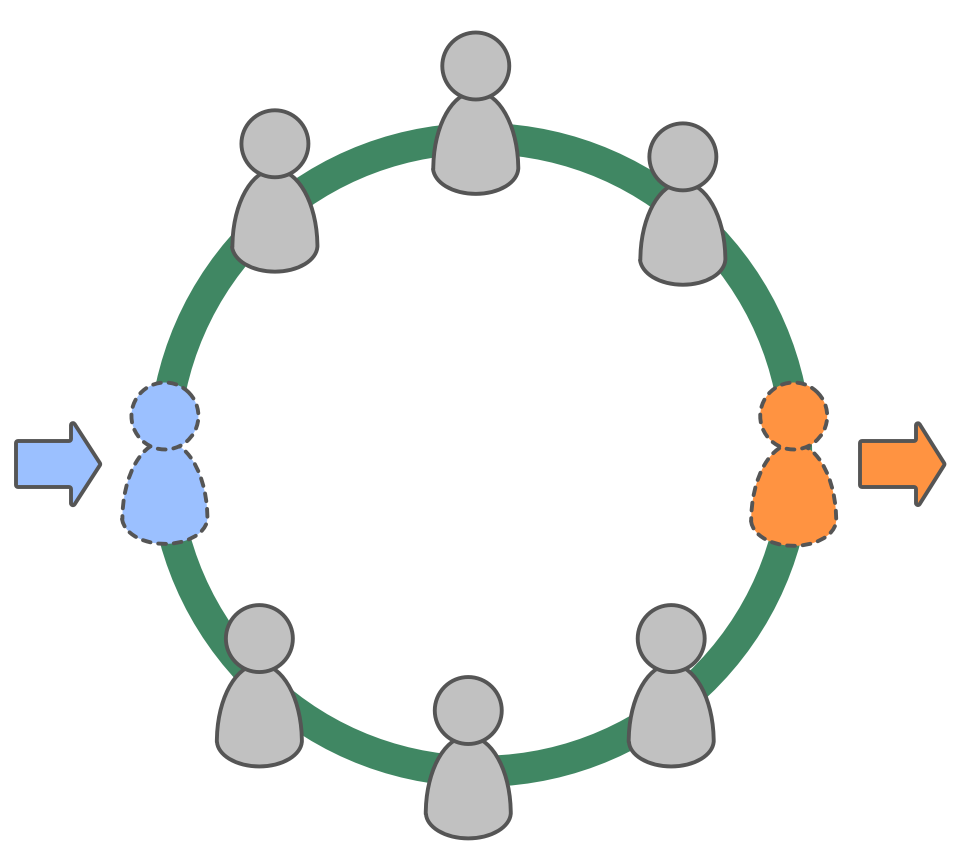
\includegraphics[keepaspectratio,width=\textwidth,height=0.75\textheight]{img/circle/enter-leave-circle.png}
\end{figure}

\begin{itemize}
\item define the process for entering the organization

\item define default role for a new member

\item define the process for leaving an organization

\end{itemize}

\section{Linking}
\label{linking}

\subsection{Connecting two circles}
\label{connectingtwocircles}

\begin{figure}[htbp]
\centering
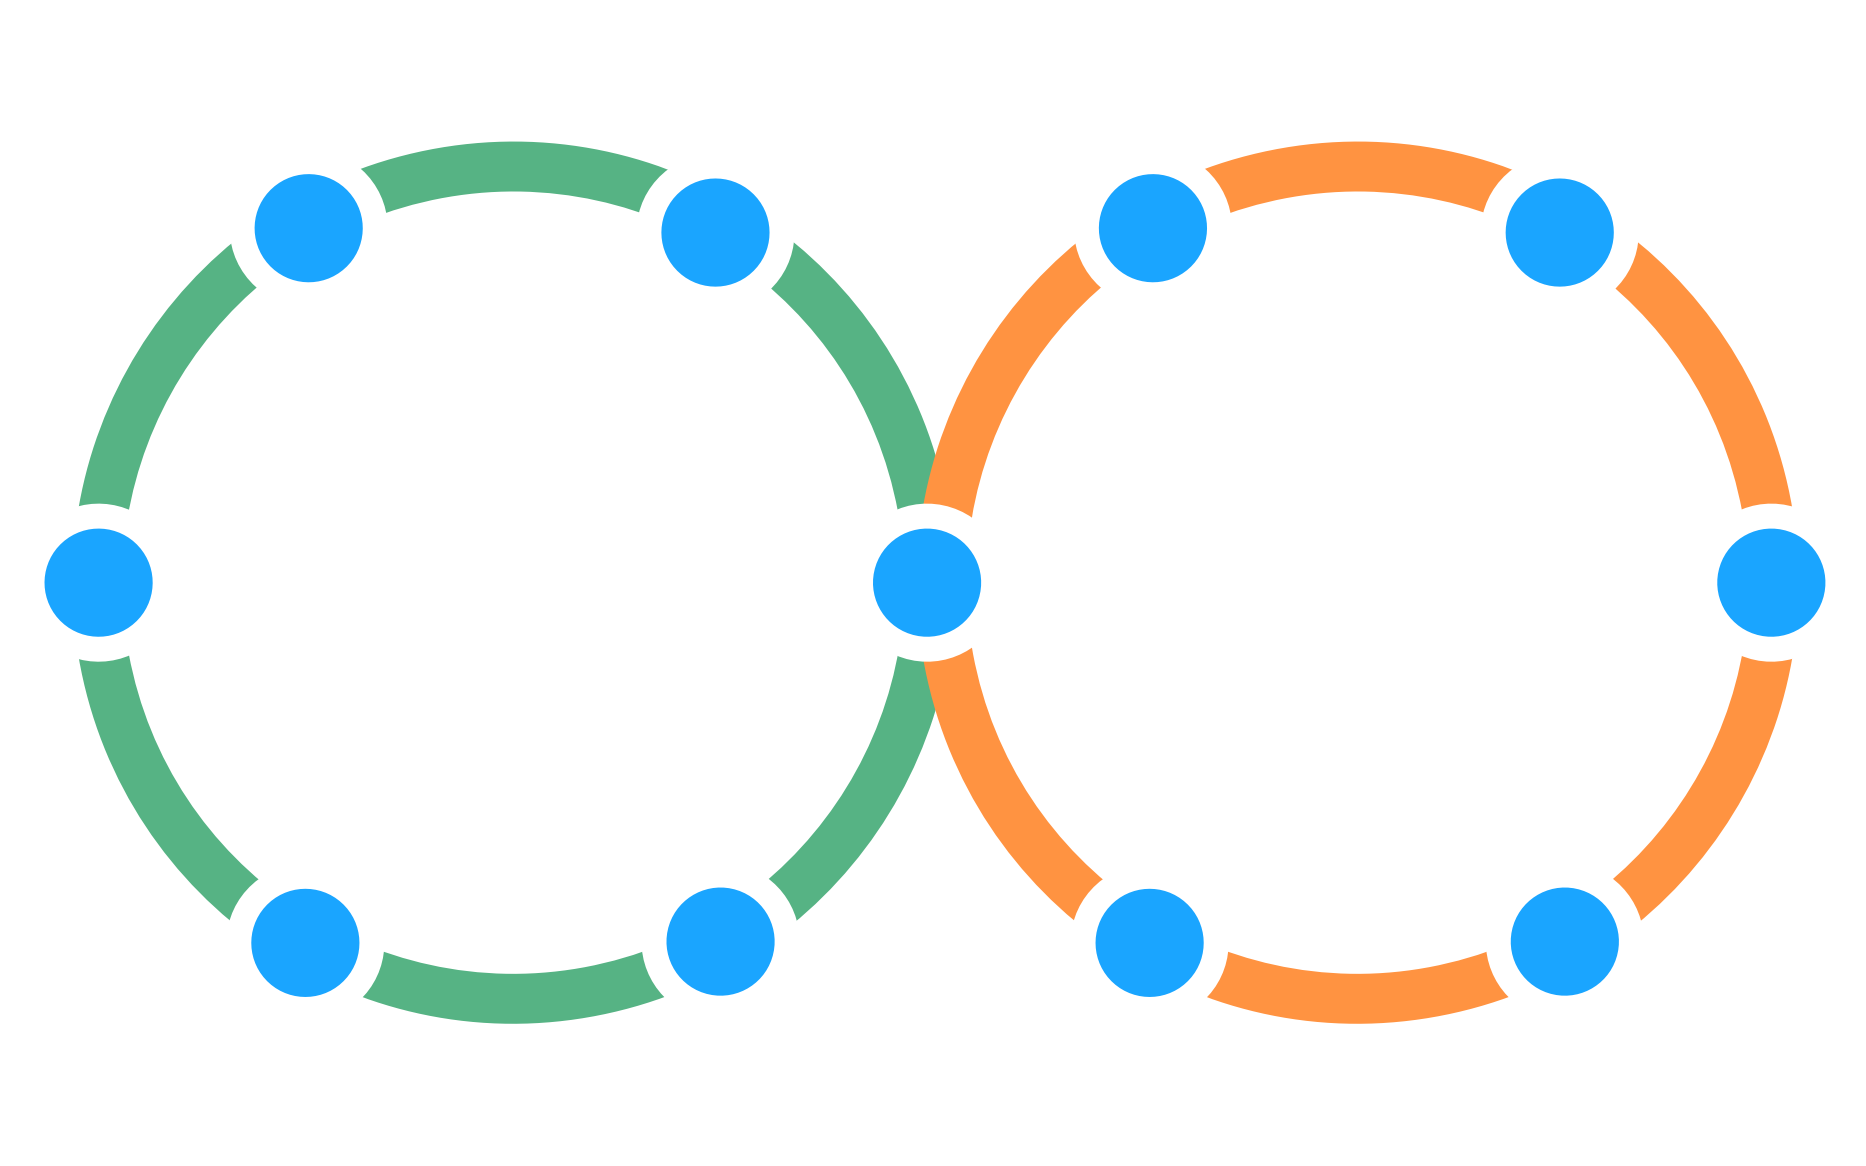
\includegraphics[keepaspectratio,width=\textwidth,height=0.75\textheight]{img/structural-patterns/link.png}
\end{figure}

\section{Transparent Salary}
\label{transparentsalary}

\begin{itemize}
\item transparent salaries need to be fair

\item perception of fairness is specific to organization

\item consider members and relevant stakeholders (e.g. investors)

\item classic sociocracy: everyone feels gains and losses

\item consider remuneration for changing roles

\item create strategy for transitioning towards new contracts and compensation agreements

\end{itemize}

\begin{figure}[htbp]
\centering
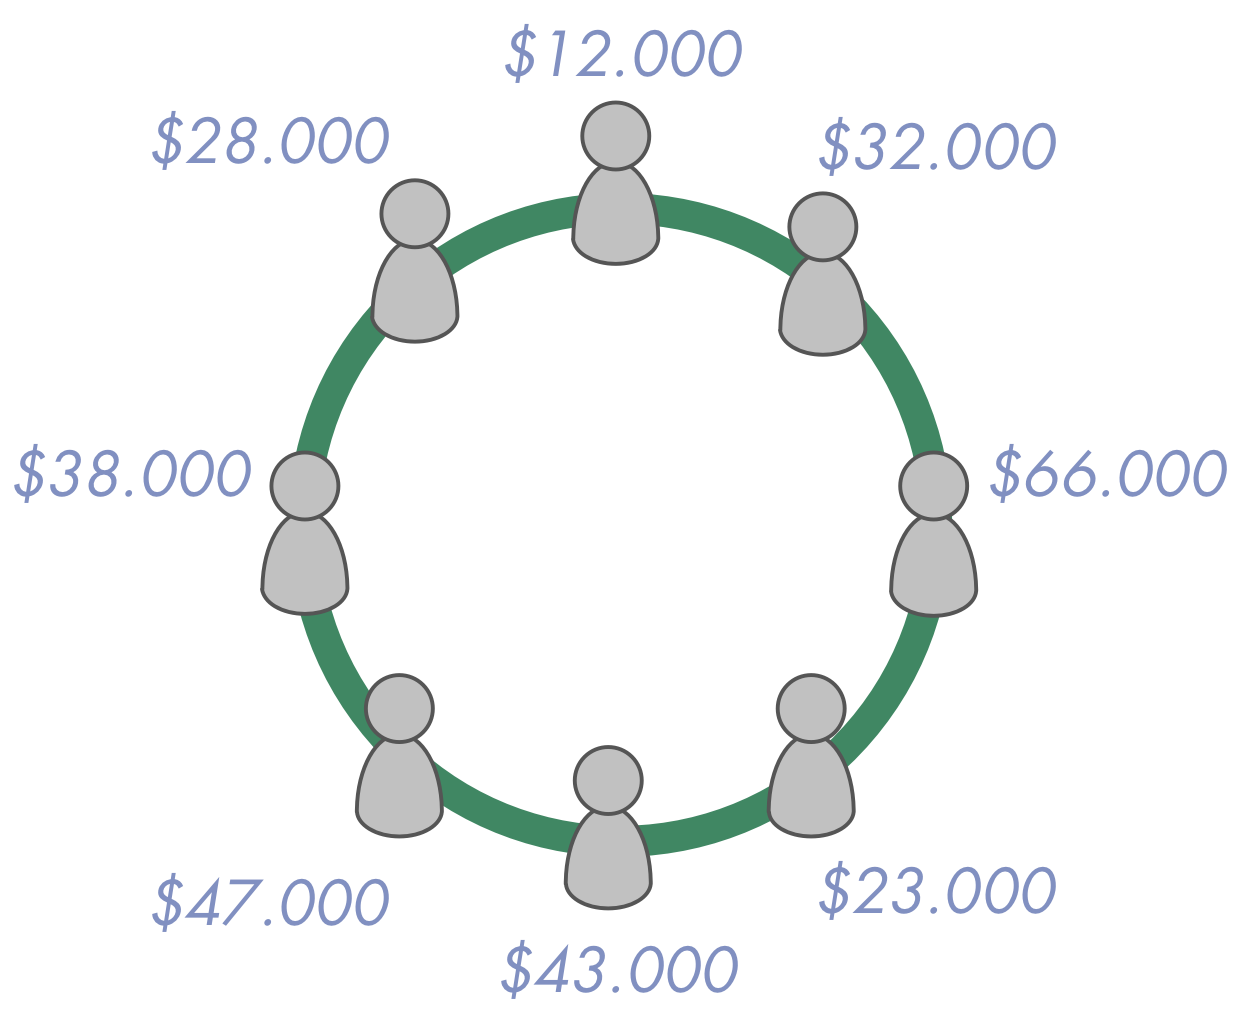
\includegraphics[keepaspectratio,width=\textwidth,height=0.75\textheight]{img/circle/transparent-salary.png}
\end{figure}

\part{Appendix}
\label{appendix}

\chapter{Changelog}
\label{changelog}

\textbf{2016--2--29}

\begin{itemize}
\item cleaned up image folder

\end{itemize}

\textbf{2016--01--28}

\begin{itemize}
\item Conversion of the material contained in the ``Introduction to Sociocracy 3.0'' slide deck

\end{itemize}

\textbf{2016--01--27}

\begin{itemize}
\item Initial setup of the patterns repository.

\end{itemize}
